\documentclass[10pt,twocolumn]{scrartcl}
\usepackage[a4paper,right=1.5cm, left=1.5cm, top=1.5cm, bottom=2cm]{geometry}
\setlength{\parskip}{1em}
\newcommand{\angstrom}{\textup{\AA}}
\usepackage{lipsum}
\usepackage[pdftex]{graphicx} 
\usepackage{url} 
\usepackage{lipsum} 
\usepackage{float}
\usepackage{amsmath}
\usepackage{amssymb}
\usepackage{amsthm}
\usepackage{subcaption}
\usepackage{mwe}
\usepackage{multicol}
\setlength{\abovedisplayskip}{2pt}
\setlength{\belowdisplayskip}{2pt}
\usepackage{tabularx}
\usepackage{longtable}
\usepackage{chemformula}
\usepackage[version=3]{mhchem}

\usepackage{listings}
\usepackage[T1]{fontenc}
\usepackage{color, listings}
\usepackage{bigfoot}
\usepackage[framed]{matlab-prettifier}
\let\ph\mlplaceholder % shorter macro
\lstMakeShortInline"
\lstset{
  style              = Matlab-editor,
  basicstyle         = \small\mlttfamily,
  escapechar         = ",
  mlshowsectionrules = true,
}

\usepackage[font={small,it}]{caption}
\captionsetup[figure]{format=plain}

\usepackage[sorting=none]{biblatex} %Imports biblatex package
\addbibresource{references.bib}
\usepackage{color} %red, green, blue, yellow, cyan, magenta, black, white
\definecolor{mygreen}{RGB}{0,0,0} % color values Red, Green, Blue
\definecolor{mylilas}{RGB}{170,55,241}
\usepackage{mathtools}
\renewenvironment{abstract}
 {\quotation\large\noindent\rule{\linewidth}{.5pt}\par\smallskip
  {\centering\bfseries\abstractname\par}\medskip}
 {\par\noindent\rule{\linewidth}{.5pt}\endquotation}
 
% hyperref color
%\usepackage{xcolor}
\definecolor{linkcolour}{rgb}{0,0.2,0.6}
\usepackage{hyperref}
\hypersetup{colorlinks,breaklinks,urlcolor=linkcolour, linkcolor=linkcolour,,citecolor=black }

\usepackage{float}

\usepackage{adjustbox}

\usepackage[title]{appendix}


\begin{document}
\renewcommand{\refname}{References}
\begin{titlepage}

\begin{center}


\includegraphics[width=0.25\textwidth]{img/collegecrest.png}\\
\vspace{3em}

\huge\textbf{Microneedle Biosensors for Measurement of Biomarkers for Sepsis and Modelling of Electron Transfer in Aptamer-based Biosensors}\\
\vspace{1em}
% {\normalsize {\textbf Danny O'Hare}\\}
%  \vspace{1em}
{\Large{\textbf{Department of Bioengineering \\ Imperial College London}}}\\[0.5in]

{\large\emph{A Project Report Submitted in \\Partial Fulfilment of the \\ \vspace{.4cm}
MEng Biomedical Engineering \\ \textsc{and}\\\vspace{-.32cm} Intercalated BSc Medical Sciences with Biomedical Engineering Degree}}
\vspace{1in}

      
\normalsize {\textbf{Supervisor:}} \\
Professor Danny O'Hare\\
\vspace{1em}
Department of Bioengineering\\
% \vspace{1em}
\url{d.ohare@imperial.ac.uk}\\
\vspace{1.5cm}
\textsc{\underline{Word count:} 4838 words}
\vfill
April, 2022
\end{center}
\clearpage
\section*{Acknowledgements}
We would firstly like to sincerely thank Prof. Danny O'Hare for supervising us throughout this entire project. His guidance has tremendously contributed to our knowledge in the field of biosensors.\\\\
Secondly, we would like to express our gratitude to Dr Sally Gowers, Mr James Mcleod, Miss Shulin Zhang, Miss Saylee Jangnam, and Miss Sanziana Foia for accommodating us in the B105 biosensor lab and for their guidance in the usage of various experimental equipment and software. We are grateful for their technical support in our experimental and modelling work.\\\\
We would lastly also like to thank Dr Tom Ouldridge for inspiring our work on coarse-grained modelling.
\tableofcontents
\end{titlepage}
 
\twocolumn[
\begin{@twocolumnfalse}
	\title{Microneedle Biosensors for Measurement of Biomarkers for Sepsis and Modelling of Electron Transfer in Aptamer-based Biosensors}
	\begin{center}
	    \author{Binghuan Li, Safiyya Musa, Anastasia Sysoeva, Danielle Tan, James Tang, \\ Peter Xie}    
	\end{center}
\maketitle
\begin{abstract}
Sepsis is defined as a life-threatening organ dysfunction caused by a dysregulated host response to infection. It is one of the primary causes of death among the critically ill. Hence, early diagnosis is vital to avoid delay in starting appropriate treatment \cite{teggert2020biomarkers}. Electrochemical microneedle (MN) biosensors have the capability for minimally invasive, continuous monitoring of sepsis biomarkers in the skin interstitial fluid (ISF), facilitating early diagnosis of sepsis. In this report, we studied three sepsis biomarkers: (1) nitrite, (2) hydrogen peroxide, and (3) lactate. Linear calibrations for nitrite were obtained using differential pulse voltammetry. Effects of albumin interference was also tested. Hydrogen peroxide in concentrations of 0 to 300uM was measured using chronoamperometry. Linear calibrations obtained from coulometry showed significant increase in charge with increasing hydrogen peroxide concentration. Lactate measured using amperometry with a rotating-disk-electrode (RDE) instrumentation and using lactate oxidase as the coating enzyme optimised our detection range of lactate concentrations covering both healthy and septic levels. We also present a modelling framework for analysis of chronoamperometric experiments performed on aptamer-based biosensors. This model presents a novel numerical inverse Laplace algorithm, capable of decomposing representative values of rate constants ($k_{A}$ and $k_{AT}$) \cite{arroyo2018subsecond}. Parameter optimisation and testing was performed to evaluate the accuracy of the multiexponential decomposition algorithm using simulated data with representative noise levels. Then, a physical coarse-grained model of the aptamer in it's target bound and unbound configurations was created. We have also comprehensively evaluated MN-based diagnostic platforms and assessed various translational challenges for MNs to be widely adopted for diagnosis of sepsis.

%Future work on modelling the chemical and physical behaviors of the aptamer  will help scientists in this field to better assess the performance of specific aptamers in molecular sensing.
\end{abstract}
\end{@twocolumnfalse}]
\section{Introduction}
\subsection{Project Aim}
At a time when demand for healthcare is rapidly increasing, healthcare systems globally are struggling with depleting resources. However, early accurate diagnosis of sepsis is vital as each hour of delay in initiating antibiotic therapy increases mortality by 5–10$\%$ \cite{heikenfeld2018lab,bauer2010molecular}. Diagnosis of sepsis is not straightforward and interpreting clinical signs and symptoms is a challenge resulting in a potential delay in diagnosis. Uncertainty about diagnosis is mitigated by needless antimicrobial therapy or the use of broad-spectrum antibiotics but this gives rise to antibiotic resistance \cite{hung2020current}. Currently, there is no gold standard for diagnosing sepsis and constant monitoring by medical staff is required. Therefore, our research aims to develop an on-body portable and wearable biosensing point-of-care (POC) MN device for infection diagnostics that can be self-managed by the public and is capable of real-time detection with high specificity and sensitivity. The device detects sepsis biomarkers in skin ISF as it mirrors blood composition; It allows the device to be small, thus, enabling it to avoid contact with nerve endings and blood capillaries, making it tolerable by patients \cite{liu2020microneedles}. \autoref{Appendix_A} provides a more comprehensive evaluation for utilising skin ISF as the target biofluid source.\\\\
Our project focuses on electrochemically detecting different sepsis biomarkers: 1) Nitrite, 2) Hydrogen Peroxide, and 3) Lactate. We studied a panel of sepsis biomarkers in order to diagnose sepsis with high specificity. In addition, this project aims to develop more representative models for aptamer-based biosensors interrogated using chronoamperometry. This method of detection allows drift-free, sub-second resolved measurements of the target molecule \cite{arroyo2018subsecond}. More accurate and representative modelling of the aptamers and their output signals will improve the precision of biomarker measurements.\\\\ 

\newpage
\section{Background}
\vspace{-0.5cm}
\subsection{Microneedles as Biosensors}
\vspace{-0.5cm}
%Microneedle-based diagnostic platforms can be divided into three main categories: biofluid extraction involving direct extraction of skin ISF with hollow and hydrogel MNs, specific target analyte capture and electrochemical biosensing with solid and hollow MNs acting as an electrode base for further modification \cite{dixon2021microneedle}.
For continuous monitoring, electrochemical MN biosensors are used which consists of a signal transducer (the MN) coated with a recognition element (nucleic acid aptamers, etc.) that forms specific interactions with the target biomarker, transmitting a quantifiable electrical signal that correlates with the target’s concentration.
\begin{center}
    \begin{figure}[H]
    \centering
    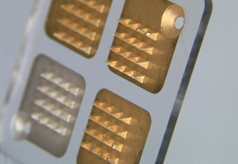
\includegraphics[width=.4\textwidth]{img/microneedle_patch.png}
    \caption{Example Image of a Microneedle array for for real-time, minimally invasive drug monitoring of phenoxymethylpenicillin \cite{rawson2019microneedle}}
    \label{fig:microneedle}
\end{figure}
\end{center}
\vspace{-1cm}
% Signal quantifying techniques include amperometry, voltammetry, potentiometry and impedance spectrometry. Voltammetric or amperometric sensors measure current changes caused by redox reactions. Potentiometric sensors measure changes in potential caused by local ion flux from target interactions. Impedance-based biosensors measure changes in resistance at the electrode surface using alternating currents.\\\\
Our MN biosensor has two main application purposes: (1) accessing the ISF by penetrating the stratum corneum into the viable epidermis and (2) act as a platform for the recognition element. Hence, more holistic theoretical research has been performed on skin structure and MN design considerations for translation to in-vivo testing in Appendix Part A and B.
\subsection{Nitrite Investigations}
Nitrite has been found to be a more sensitive and specific biomarker for diagnosing septic shock compared to known biomarkers such as procalcitonin, C-reactive protein and interleukin-6, and its concentration remains elevated days after admission \cite{pmid9142024}.\\\\
We aim to measure nitrite concentration in solution by performing a differential pulse voltammogram, followed by obtaining a calibration curve, examining the reduction of nitrite (NO$^{2-}$) to nitrate (NO$^{3-}$), shown in \autoref{eqn:nitriteredox1} and \autoref{eqn:nitriteredox2}.
\begin{align} \label{eqn:nitriteredox1}
   NO\textsubscript{2}\textsuperscript{-} \ \xrightleftharpoons{}  NO\textsubscript{2} \ + \  e\textsuperscript{-}
\end{align} 
\begin{align}\label{eqn:nitriteredox2}
  2NO\textsubscript{2} \ + \ H\textsubscript{2}O \xrightarrow{}\  2H\textsuperscript{+} \ + \ NO\textsubscript{2}\textsuperscript{-} \ + \  NO\textsubscript{3}\textsuperscript{-}
\end{align}
Differential pulse voltammetry (DPV) measures the concentration of electrolytes in solution by applying potential (E) at the working electrode (WE) and reference electrode (RE). A series of pulses of increasing steps is applied to the WE and the difference in current between steps is measured \cite{D1CP00661D}. A calibration curve is then constructed from the peaks of the curve using linear regression. \\\\
Experiments utilising disposable gold electrodes, where the WE, RE and CE are all located on a 10mm x 8mm polycarbonate surface were then performed. These electrodes have been shown to have good electrochemical response, as well as being cheap and disposable, favouring use in a clinical setting as a biosensor \cite{FERRARIO201236}.\\\\
Albumin is found in human blood in the range of 33–52 g/L. There is some evidence that presence of albumin may interfere with electrode activity, which may be due to precipitate forming on the electrode surface, thus reducing surface area \cite{doi:10.1177/000456329102800111}.
%======================================================================================================
\subsection{Hydrogen Peroxide Investigations}
Hydrogen peroxide, H\textsubscript{2}O\textsubscript{2}, is a chemical that is commonly found in multiple biological processes \cite{Pravda2014}. It is reported that a drastic increase of the \textit{in vivo} hydrogen peroxide concentration is usually accompanied with systemic inflammations. From previous research, an approximate 10-fold increase in hydrogen peroxide concentration was observed, from 21-36uM in blood from healthy individuals \cite{FORMAN201648}, to 316$\pm$242.8uM in septic blood \cite{VanAsbeck1995}. Therefore, hydrogen peroxide serves as a novel sepsis biomarker that demonstrates high suitability for clinical continuous-monitoring techniques using microneedles.  Its capability in identifying sepsis and indicating severity of infection provides a high significance in sepsis diagnosis, evolution evaluation and prognosis prediction.\\\\
\noindent To detect hydrogen peroxide, a strategy based on reduction-oxidation (redox) reactions between hydrogen peroxide and Prussian blue (PB) is proposed by Chen \textit{et al} \cite{C9AN02438G}. Prussian blue, also known as ferric ferrocyanide, is an artificially synthesised chemical complex that demonstrates an outstanding hydrogen peroxide sensing range with low operating potential. This two-step reaction commences by reducing Prussian blue to Prussian white (PW) (shown in \autoref{eqn:h2o2redox1}) where hydrogen peroxide is further reduced to water (shown in \autoref{eqn:h2o2redox2}).
\begin{align} \label{eqn:h2o2redox1}
    KFe^{3+}[Fe\textsuperscript{2+}(CN)\textsubscript{6}]\textsuperscript{4-} \ + \ & K\textsuperscript{+} \ + \   e\textsuperscript{-} \ \xrightleftharpoons{} \\ \nonumber & K\textsubscript{2}Fe\textsuperscript{2+}[Fe\textsuperscript{2+}(CN)\textsubscript{6}]\textsuperscript{4-}
\end{align}
\begin{align} \label{eqn:h2o2redox2}
    & 2K\textsubscript{2}Fe\textsuperscript{2+}[Fe\textsuperscript{2+}(CN)\textsubscript{6}]\textsuperscript{4-} \ + \  H\textsubscript{2}O\textsubscript{2} \ + \ 2H\textsuperscript{+} \ \xrightleftharpoons{} \\ \nonumber & \quad \quad 2K\textsubscript{2}Fe\textsuperscript{3+}[Fe\textsuperscript{2+}(CN)\textsubscript{6}]\textsuperscript{4-} \ + 2H\textsubscript{2}O \ + \ 2K\textsuperscript{+}
\end{align}
\noindent A graphical visualization to the reactions between H\textsubscript{2}O\textsubscript{2} and PB can be found in \autoref{fig:pb_h2o2}.
\begin{figure}[H]
    \centering
    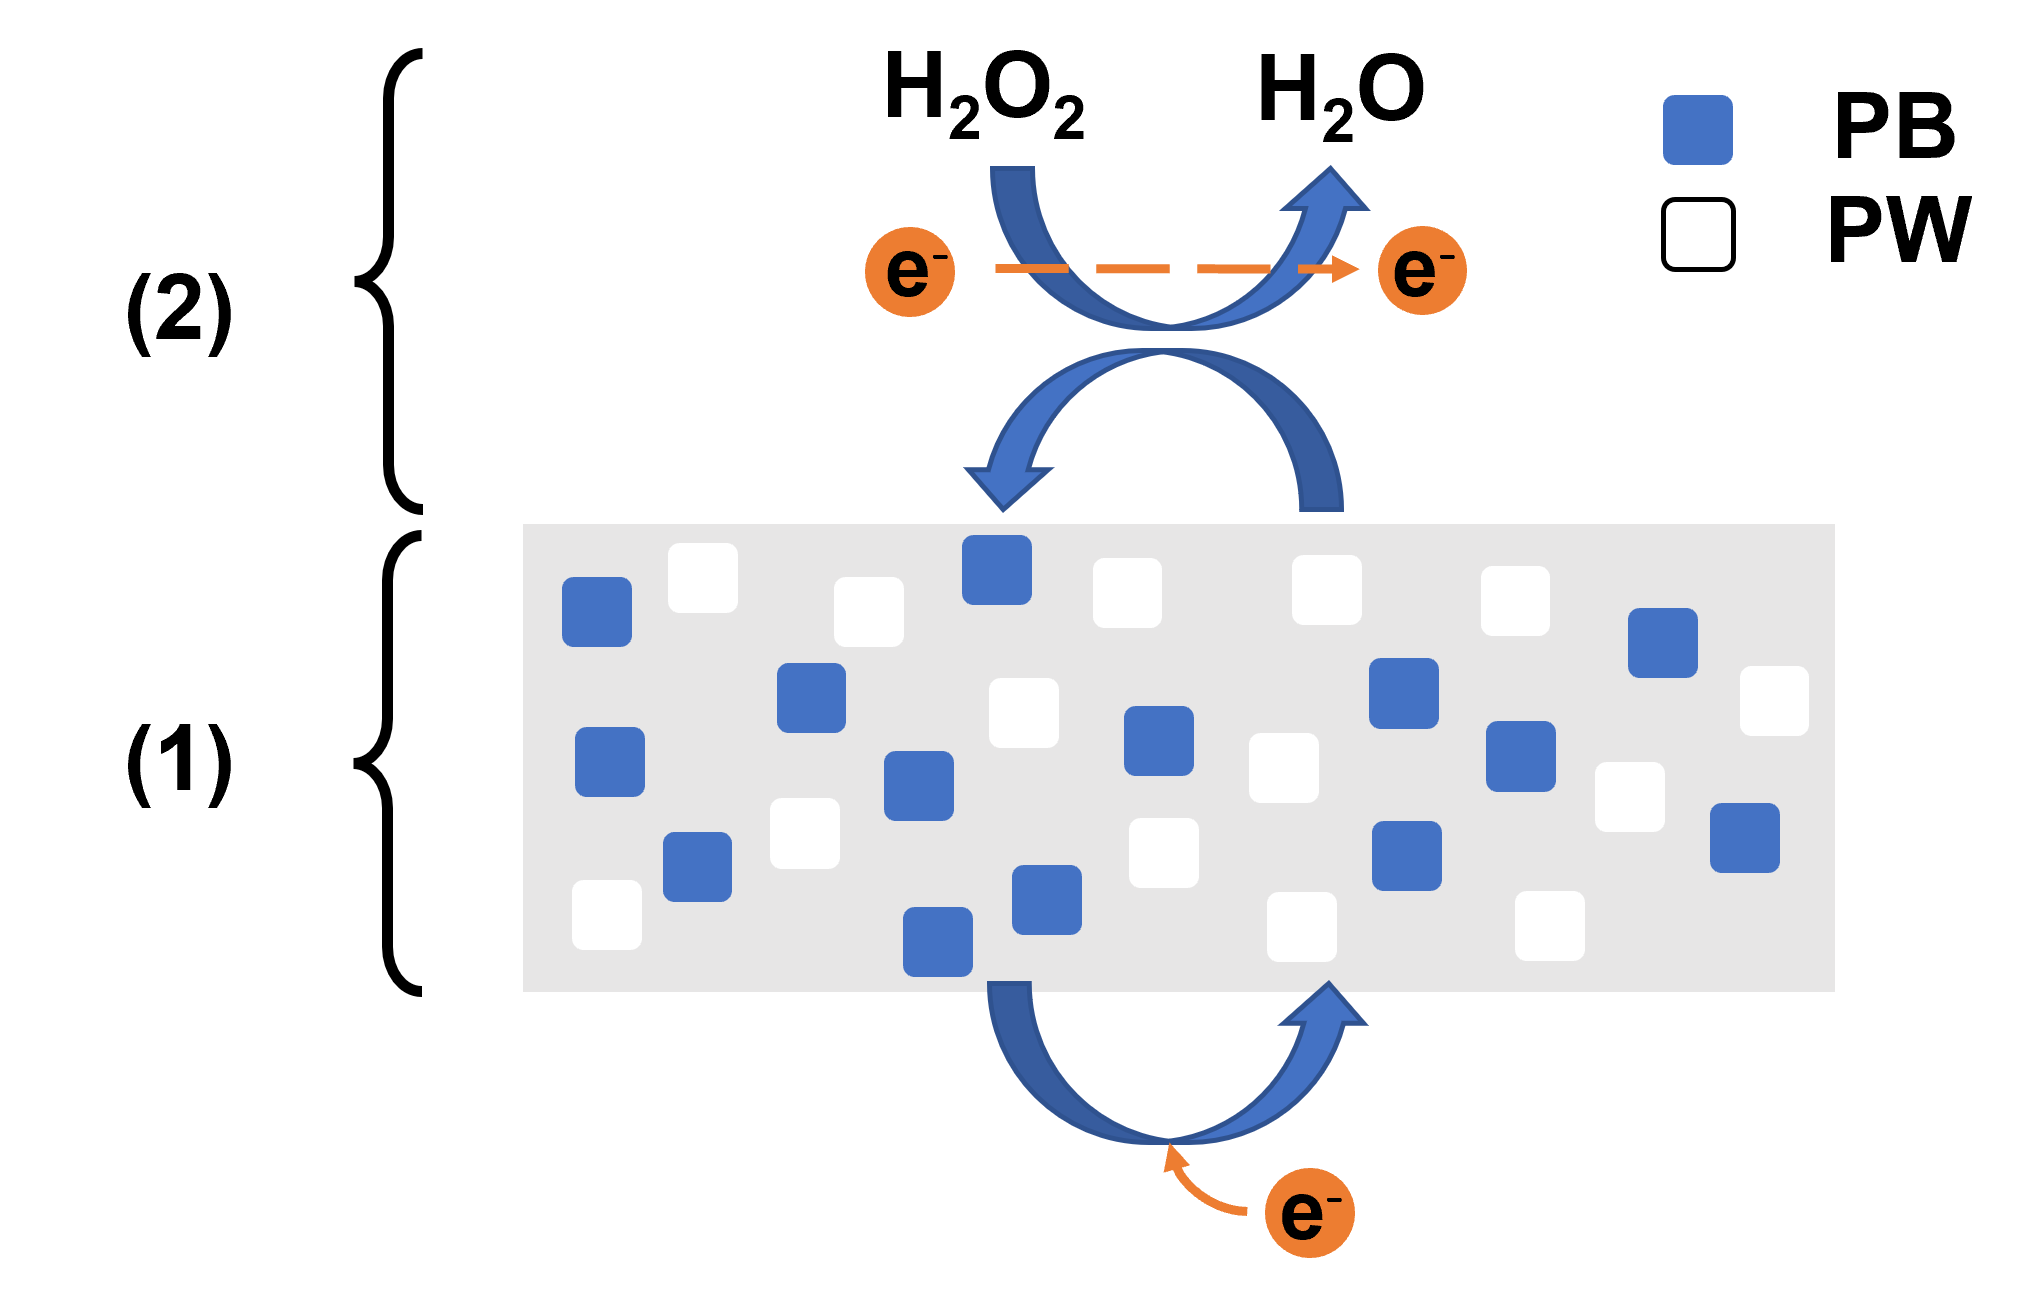
\includegraphics[width=.5\textwidth]{img/pb_h2o2.png}
    \caption{Reaction between hydrogen peroxide and Prussian blue.}
    \label{fig:pb_h2o2}
\end{figure}
%======================================================================================================
\subsection{Lactate Investigations}
Patients suffering from sepsis often develop Sepsis-Associated HyperLactatemia (SAHL). SAHL can be explained by multiple proposed theories. The least contested and most evidential blames the increase of aerobic glycolysis rates, subsequent to adrenergic stimulation, for SAHL \cite{garcia2014sepsis}.
Hyperlacatatemia can be characterised most commonly by a serum concentration exceeding 4mM however different literature suggests lower thresholds beginning at 3mM can also indicate a significant septic state \cite{singer2014ed}.
Therefore, real-time monitoring of lactate levels in clinical settings is vital whereby levels exceeding those of healthy patients or sharp increases can be detected quickly for antibiotics administration or other appropriate measures to be taken before fatal state is reached \cite{gyawali2019sepsis}.
In this project, we aim to develop enzyme-based electrode that can detect lactate levels of both healthy and septic patients in the 0.0-4.5mM.
\subsection{Statistics of Diagnosis}
When working with different biomarkers of sepsis it is critical that readings are specific and predictive. Particularly in the case of sepsis, treatment includes administration of antibiotics; If antibiotics are delivered unnecessarily, it could lead to antibiotic resistance.\\\\
To evaluate the success of a biomarker at positively indicating disease the sensitivity, specificity, predictive values and diagnostic accuracies are statistics commonly used amongst clinicians to quantify the success of the diagnostic technique at mitigating false results. To calculate each of these variables, the biomarker must be assessed for both false and true positives and negatives against a pre-established gold standard diagnosis (assumed 0 false positives). Sensitivity can be described as the ratio of observed positives to all the real number of positives (true positives/true positives + false negatives), it indicates how well the biomarker picks up disease \cite{kazmierczak1999statistical}. \\\\
Specificity is given by the ratio of true negatives observed to the actual number of negative cases (true negatives/true negatives + false positives). For particular biomarkers which can be used for various disease, the specificity can be considerably lower, owing to the higher rate of false positives. The positive predictive value gives the ratio of true positives to total positives observed (true positives/ false and true positives), whereas the negative predictive value gives the ratio of true negatives to total negatives observed (true negatives/ false and true negatives).  The overall diagnostic accuracy is given by the proportion of all true results \cite{christenson2007evidence}.\\\\
For both predictive values and overall diagnostic accuracies, variations occur with prevalence of sepsis. PPV can increase dramatically with increase prevalence and so often sensitivity and specificity are more frequently used to describe efficacy of detection methods. However, these are not immune to variability- especially in the case of sepsis. Sepsis is not always binary, it may be that a patient is at risk of septic shock or approaching levels that are indicative of entering septic shock but are not septic in that moment. In such cases a ‘cut off mark’ is not always a singular number but more often a range and often these ranges are disputed and unclear in literature \cite{xia2013translational}. \\\\
Perhaps a more useful and less discriminatory way at quantifying usefulness is looking at the relationship between sensitivity and specificity by plotting receiver operating characteristics (ROC). Where there exists a range of values rather than a single cutoff value, sensitivity and specificity value pairs can be determined for different levels of biomarker concentration. By plotting 1-specificty versus sensitivity we can obtain a ROC curve. The shape of the curve (i.e asymmetry) and the area under it, can both be used in conjunction to convey diagnostic accuracy and allow clinicians to contextualise and make decisions from the results our sensors give \cite{kampfrath2013brief}. 
\subsection{Aptamer-Based Biosensors}
% Nucleic acid aptamers are short single stranded oligonucleotides sequences that will selectively bind to specific target molecules such as biomarkers, metal ions, antibiotics and more with high affinity and specificity. They are selected using SELEX. Once the nucleic acid sequence is chosen, it can be synthesised and modified with a redox-active group. Upon binding to the target, aptamers can undergo different types of conformational changes forming structural shapes such as hairpins, bulges, and G-quadruplexes  \cite{riccitelli2010computational}. This results in a change in the distance between the redox group and electrode surface which thus leads to a change in the current.\\\\
Nucleic acid aptamers exhibit many advantages as biorecognition elements in biosensing compared to other sensing molecules such as enzymes and antibodies. They are small in size, chemically stable and cost effective \cite{song2008aptamer}. Aptamers can be isolated from a library of sequences via SELEX, and can selectively bind to many different types of small molecules such as biomarkers, metal ions, antibiotics and more \cite{cai2018investigations}. Aptamers can undergo different types of conformational changes upon target binding to form structural shapes such as hairpins, bulges, and G-quadruplexes \cite{riccitelli2010computational}. This conformational change results in a change in distance between the modified redox group and electrode surface which thus leading to a change in the current.\\\\
% The anatomy of DNA-based biosensors contains three major elements, an electrode-blocking self-assembled monolayer (SAM) used to prevent the occurrence of undesired electrochemical reactions,
% a SAM functionalized with aptamers, and a redox reporter to allow detection of binding-induced conformational changes in the aptamer \cite{pellitero2019critical}. Interrogating aptamer-based sensors using chronoamperometry and chronocoulometry as electrochemical methods allows direct monitoring of target binding-induced changes in the electron transfer rate from the redox reporter \cite{arroyo2018subsecond}. In response to a potential step in the working electrode, chronoamperometry measures the current transient, while chronocoulometry measures the cumulative charge. These electrochemical methods have significant advantages over voltammetric detection methods such as square wave voltammetry (SWV) \cite{white2010exploiting} and cyclic voltammetry \cite{fan2003electrochemical}. These methods are dependant on parameters such as the number of redox-reporter molecules intercelated on the aptamer, as well as the density of adsorbed aptamers. These can vary from sensor to sensor due to fabrication variations. Chronoamperometric detection also offers drift resistant measurements and subsecond temporal measurements of target molecules in situ. \\\\
Interrogation of aptamer-based biosensors using chronoamperometric detection offers drift resistant and subsecond temporal measurements of target molecules in situ. In Plaxco's analysis of the current transient lifetime, the initial rapid exponential phase due to the charging of the electrode double layer is ignored, and the lifetime of the slower faradic current decay (due to the electron transfer of the methylene-blue) is measured. Experimental results using tobramycin (an antibiotic used to treat bacterial infections) show a five times reduction in decay lifetime from no target to a saturated target concentration. The authors predicted the phase of exponential decay (corresponding to a single-exponential fit) varies linearly with the target concentration. The authors claimed the lifetimes for the two aptamer states to be similar, stating that it would be difficult to extract the relevant amplitudes with sufficient precision. They do not show any attempt at multiexponential decomposition to justify the proximity of the electron transfer rates. Instead, they resort to approximating the current decay lifetime using a monoexponential fit. The derivation for the multiexponential current output of aptamer-based biosensors interrogated using chronoamperometry is shown in (\autoref{Aptamer_multiexp}).\\\\
% Electron transfer is empirically a first order reaction - therefore the resultant current decay is likely a combination of two exponentials superimposed on each other. \\\\
%The assumption that the aptamers are fully bound with saturated target concentration and fully unbound in the absence of target is also invalid, as aptamers can take up different natural conformations (REFERENCE). The complete features of the aptamer behaviour are not fully considered in this study.\\\\
Multiexponential decomposition is an ill-posed problem, especially with signals with intrinsic noise. This problem is present in semiconductor physics, fluorescence decay analysis (FRET), nuclear physics and chemistry (radioactive decays, nuclear magnetic resonance), chemistry and
electrochemistry (reaction kinetics) and medical imaging \cite{jibia2012appraisal}.
In this project, we present an accurate and representative model on the analysis of chronoamperometric detection in aptamer biosensors, starting from first principles, considering the physical nature of DNA motion \cite{ouldridge2012coarse}. We connect this to the chronoamperometric signal by appropriately decomposing the general multiexponential signal using a numerical inverse Laplace method \cite{provencher1982contin} in order to extract both the bound and unbound aptamer rate constants and their respective concentrations.\\\\



\newpage
\section{Methods}
\vspace{-0.5cm}
\subsection{Nitrite Investigations}
\vspace{-0.5cm}
To obtain the voltammogram and calibration curves, DPV was performed on increasing concentrations of nitrite solution using the apparatus as described in \autoref{fig:h2o2_setup}. The solution was degassed with nitrogen gas to remove oxygen gas.\\
\begin{table}[H]
    \centering
    \begin{tabular}{ |p{3.7cm}||p{3.7cm}| } 
        \hline
        \multicolumn{2}{|l|}{\textbf{Reusable gold electrode}} \\ \hline
        Reusable gold electrode in PBS solution & Obtain baseline voltammetry and calibration curve for nitrite detection and estimate expected peaks\\ \hline
        Reusable gold electrode with 4\% albumin & Determine magnitude of effect of albumin in solution and compare to previous results \\ \hline
        \multicolumn{2}{|l|}{\textbf{Disposable gold electrode}} \\ \hline
    Disposable gold electrode in PBS solution & Obtain voltammetry and calibration curve and compare performance to reusable electrodes. \\ \hline
    Disposable gold electrode with 5.2g/L albumin & Determine magnitude of effect of albumin in solution and compare to previous results\\ \hline
    \end{tabular}
    \caption{A summary of performed experiments is shown}
    \label{tab:my_label}
\end{table}

\noindent{Detailed descriptions of performed experiments are listed in \autoref{app:nitrite_protocol}.}



\begin{figure}[H]
\centering
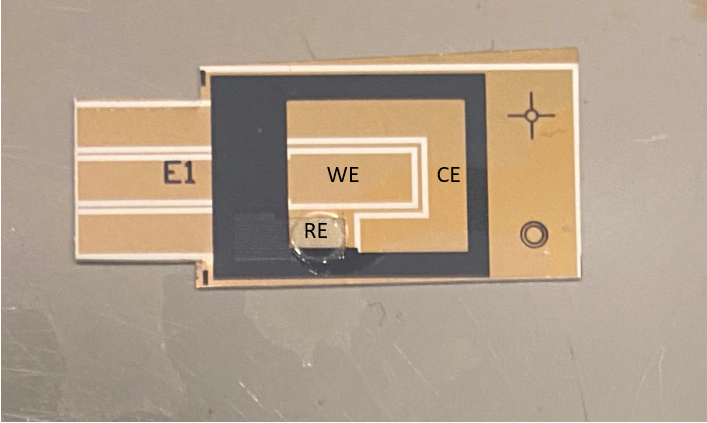
\includegraphics[width=0.45\textwidth]{img/disp electrode.PNG}
\caption{Image of gold disposable electrode. Working electrode (WE), Reference electrode (RE), Counter electrode (CE). pHEMA layer has been applied to RE. Disposable electrodes were prepared by washing in 75\% ethanol, and the RE was coated with 5$\mu$M Polyhydroxyethylmethacrylate (pHEMA) and baked for one hour at 70\textdegree{C}}
\end{figure}


\subsection{Hydrogen Peroxide Investigations}
To perform the sensing of hydrogen peroxide with Prussian blue, a four-step protocol has been established based on the publication by Chen \textit{et al.} \cite{C9AN02438G}, as shown in \autoref{app:h2o2_protocol}. Gold (Au) electrode were adopted for the calibration in the current stage. However disposable electrodes may be introduced for blood sample testing in the future work. \\\\
In the first stage of electrochemical detection, the PEDOT:PSS-PB complex has been synthesised and crosslinked with ethylene glycol (EG) and  divinyl sulfone (DVS) to improve its mechanical stability. A gold working electrode coated with PEDOT:PSS-PB-EG-DVS complex is then cured in an oven, which ensures a firm attachment of PB to the electrode.
\begin{figure}[H]
    \centering
    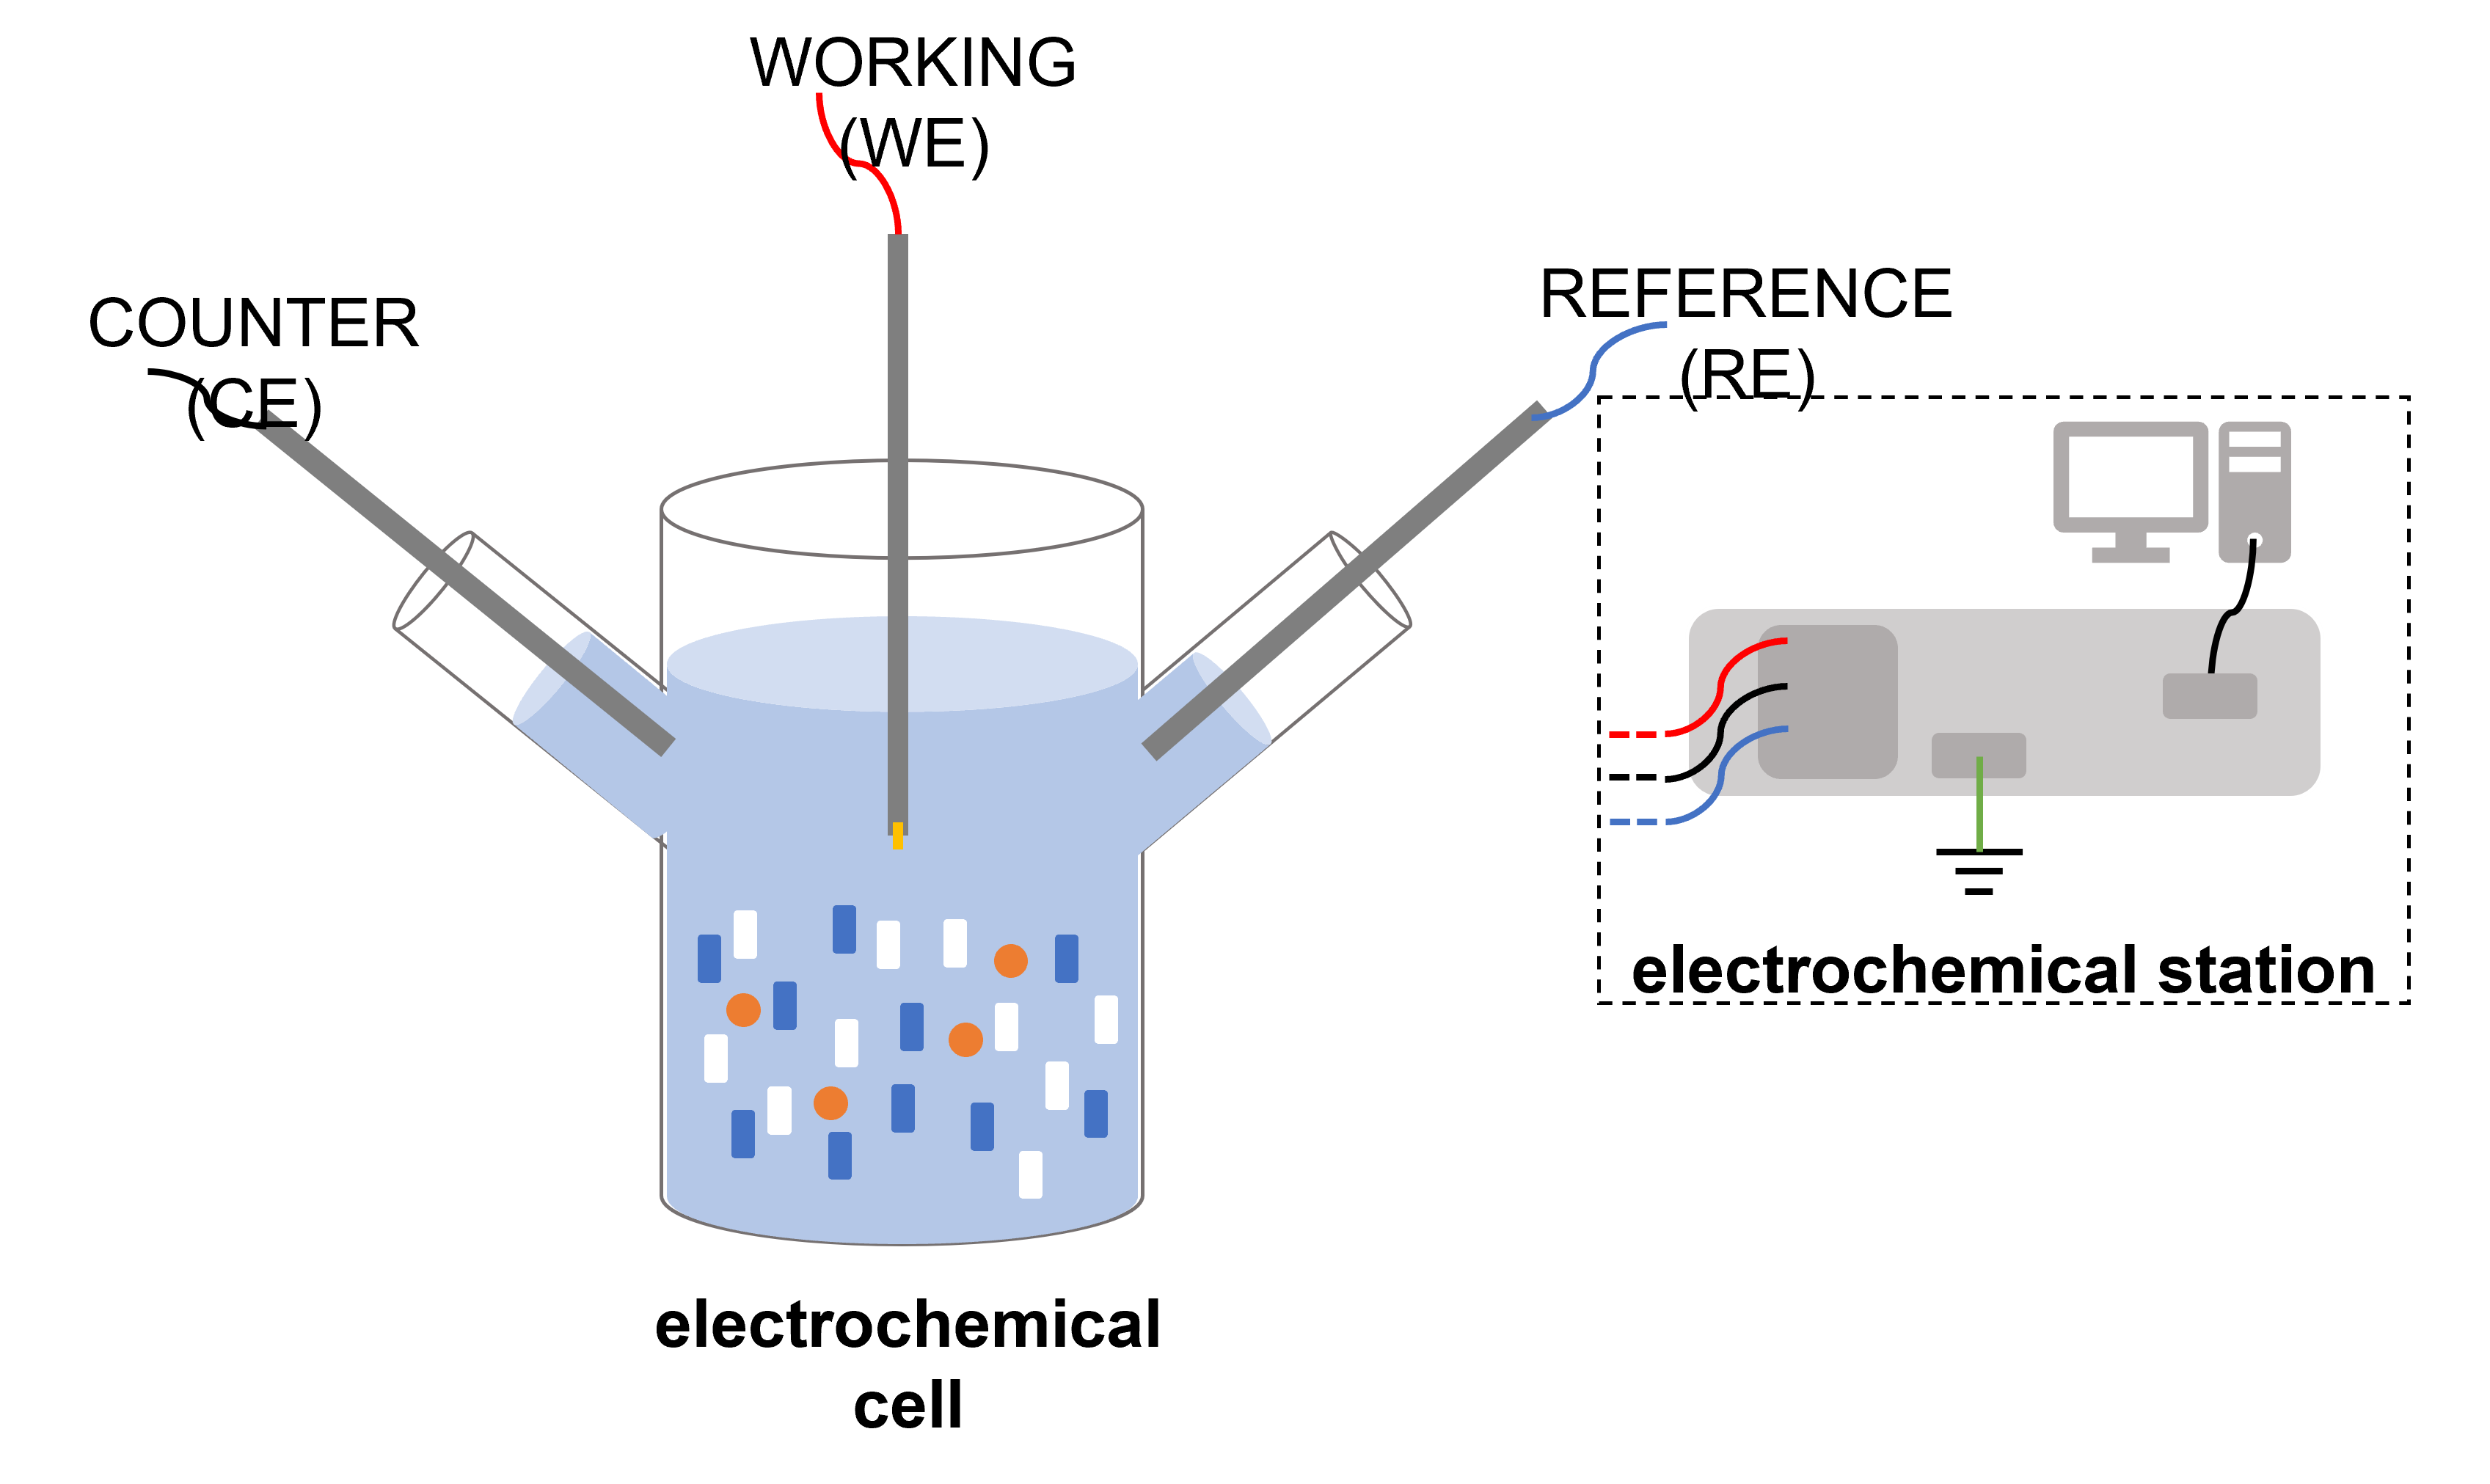
\includegraphics[width=.5\textwidth]{img/h2o2_setup.png}
    \caption{Electrochemical detection experimental setup for nitrite, hydrogen peroxide and lactate calibration}
    \label{fig:h2o2_setup}
\end{figure}
\noindent The experimental setup for hydrogen peroxide detection is shown in \autoref{fig:h2o2_setup}. Cyclic voltammetry was first performed in the blank buffer. This step is essentially a validation of the existence of PB in the reaction environment. \\\\
\noindent Chronoamperometry was performed following the cyclic voltammetry scan. Hydrogen peroxide was added to the reaction environment gradationally from 0$\mu$M to 300$\mu$M and reacted with Prussian blue. Current and time data were collected under each concentration; Coulometry was then performed for experimental validation.

%====================================================================================
\subsection{Lactate Investigations}
Ideally, our sensor would be able to detect lactate levels in the range of 0.5mmol/L to 4mmol/L; This would cover healthy and septic levels. Without modification, LOX sensors have a detection limit of 0.25mM where sites become saturated. To optimise the detection range, we need to increase the concentration at which saturation occurs. In this experiment,  Nafion, a sulfonated polymer, is coated onto the electrode surface, which leaves a negative charge in the solution, reducing the flux of lactate to the enzyme layer \cite{rathee2016biosensors} \cite{romero2010amperometric}. Further modifications to membrane thickness and enzyme type can increase our detection range. Electrodes were prepared from gold electrodes by coating with interference exclusion and enzyme hydrogel layers, see \autoref{app:lactate_protocol}.\\\\
The electrochemical cell was then set up using the lactate electrode as the working rotating disc electrode, platinum as the counter and Ag/AgCl as the working electrode with the configuration shown in \autoref{fig:h2o2_setup}.\\\\
RDE is important for enzyme sensors as it maximises the proportion of mass transport due to convection and allows for a fully defined flow pattern around the electrode \cite{nikolic2000theoretical}. Amperometry was then conducted at 0.7V and 400rpm on 7.4pH PBS solutions spiked with 0.2mM aliquots in the 0.0-3.0mM range and then 0.5mM aliquots in the 3.0-4.5mM range. \subsection{Aptamer Modelling}
\subsubsection{Numerical Inverse Laplace Algorithm}
The output current is sampled at discrete time points in chronoamperometric experiments on aptamer biosensors. We, therefore, need to adapt the NIL algorithm for discrete signals using a numerical linear least-squares approach.\\\\
For discrete signals, we can use the NIL transform to find the coefficients of the exponential decays (spectra $\mathbf{G}(k)$).
The algorithm aims to minimise the error between the model fit and the experimental data.
The discrete form of a general chronoamperometric signal can be represented as \autoref{Apt_discrete}:
\begin{equation}
    y(t_{i}) = \sum_{j=1}^{N} \mathbf{G}(k_{j})e^{-t_{i}k_{j}}
    \label{Apt_discrete}
\end{equation}
In matrix form \autoref{Apt_discrete} can be represented as:
$$ \mathbf{y = AG} $$
The minimisation becomes a linear least squares problem, which we solve using the Nelder Mead's method:
\begin{equation}
    min\lVert \mathbf{AG} - \mathbf{y}\lVert^{2}_{2}
    \label{discretething}
\end{equation}
where $\mathbf{G}$ $\in$ $\mathbf{R}^{N}$.\\\\
An additional regularizer is added to smooth the output solution.
\begin{equation}
    V(\alpha) = \lVert \mathbf{AG} - \mathbf{y}\lVert^{2}+\alpha^{2}\lVert \mathbf{r} - \mathbf{RG}\lVert  = min
\end{equation}
$\mathbf{R}$ considers prior knowledge of $\mathbf{G}(k)$. $\mathbf{r}$ represents the second derivative of $\mathbf{G}(k)$. Increasing the value of $\alpha$ favours smoother solutions, as they have smaller second derivative values. See \autoref{Aptamer_multiexp} for a detailed description of the mathematical implementation of the algorithm and \autoref{app:apt_mod} for the code to perform these simulations.\\\\
\subsubsection{Coarse-grained Modelling of Aptamers}
% \vspace{-.8cm}
To relate the electron transfer rates of the bound and unbound aptamer configurations ($k_{A}$, $k_{AT}$) to the distance between redox reporter (MB) and electrode surface, we develop a model of aptamers to predict the distribution of aptamer configurations.\\\\ 
Without considering the chemical or thermodynamic effects of base interactions within the aptamer \cite{feigon1996aptamer}, we assume the aptamers to be a freely-jointed chain where the chains can rotate with 3DOFs.
The persistence length is a mechanical property quantifying the bending stiffness of a polymer. For double-stranded DNA (dsDNA), persistence length is widely reported as 50 nm \cite{bloomfielduniversity,marko1995stretching}. The latest measurements of persistence length on single-stranded DNA (ssDNA) using atomic force microscopy shows a measurement of $1.98 \pm 0.72$nm \cite{roth2018measuring}, in the range of previously published values of 1.5 - 3nm \cite{murphy2004probing,chi2013persistence}. For pieces of ssDNA shorter than the persistence length, the molecule behaves like a rigid rod, while for pieces of the ssDNA that are much longer than the persistence length, the properties can be described statistically as a three-dimensional random walk.\\\\
For aptamers tested in the laboratory, their base numbers range from 50-100, corresponding to lengths of 17 and 34nm \cite{alberts2014molecular}, an order of magnitude larger than the persistence length of ssDNA. Therefore, we consider the aptamer as a freely-jointed chain with rigid segments of size $b = 2\zeta$ (where $\zeta$ is the persistence length, $b$ is the Kuhn length) \cite{strobl1997physics}.\\\\
In our model, we simulate random vectors in the spherical coordinate space for each rigid segment and extract the end-to-end distance from the redox reporter to the electrode surface. In cases where any of the rigid segments reach below the electrode surface ($z=0$), we instead take the absolute z-value (maintain the randomly generated theta value, and recalculate the phi value such that the Kuhn segment length is maintained) and continue the simulation. This, therefore, considers the redox reporter to bounce off the electrode. 3D simulations for 50, 100, and 200 bases (\autoref{Apt_sim}) are shown, where we plot the probability distribution for the end-to-end distance from the redox reporter to the electrode surface. \\\\
Extending the numerical simulation to 5E+06 simulations, the length distribution tends to be half-gaussian, centred at the electrode surface (z=0) (\autoref{L_dist}). The MATLAB code used to generate the stochastic models of the DNA is in \autoref{app:apt_mod}.
\begin{figure}[H]
    \centering
    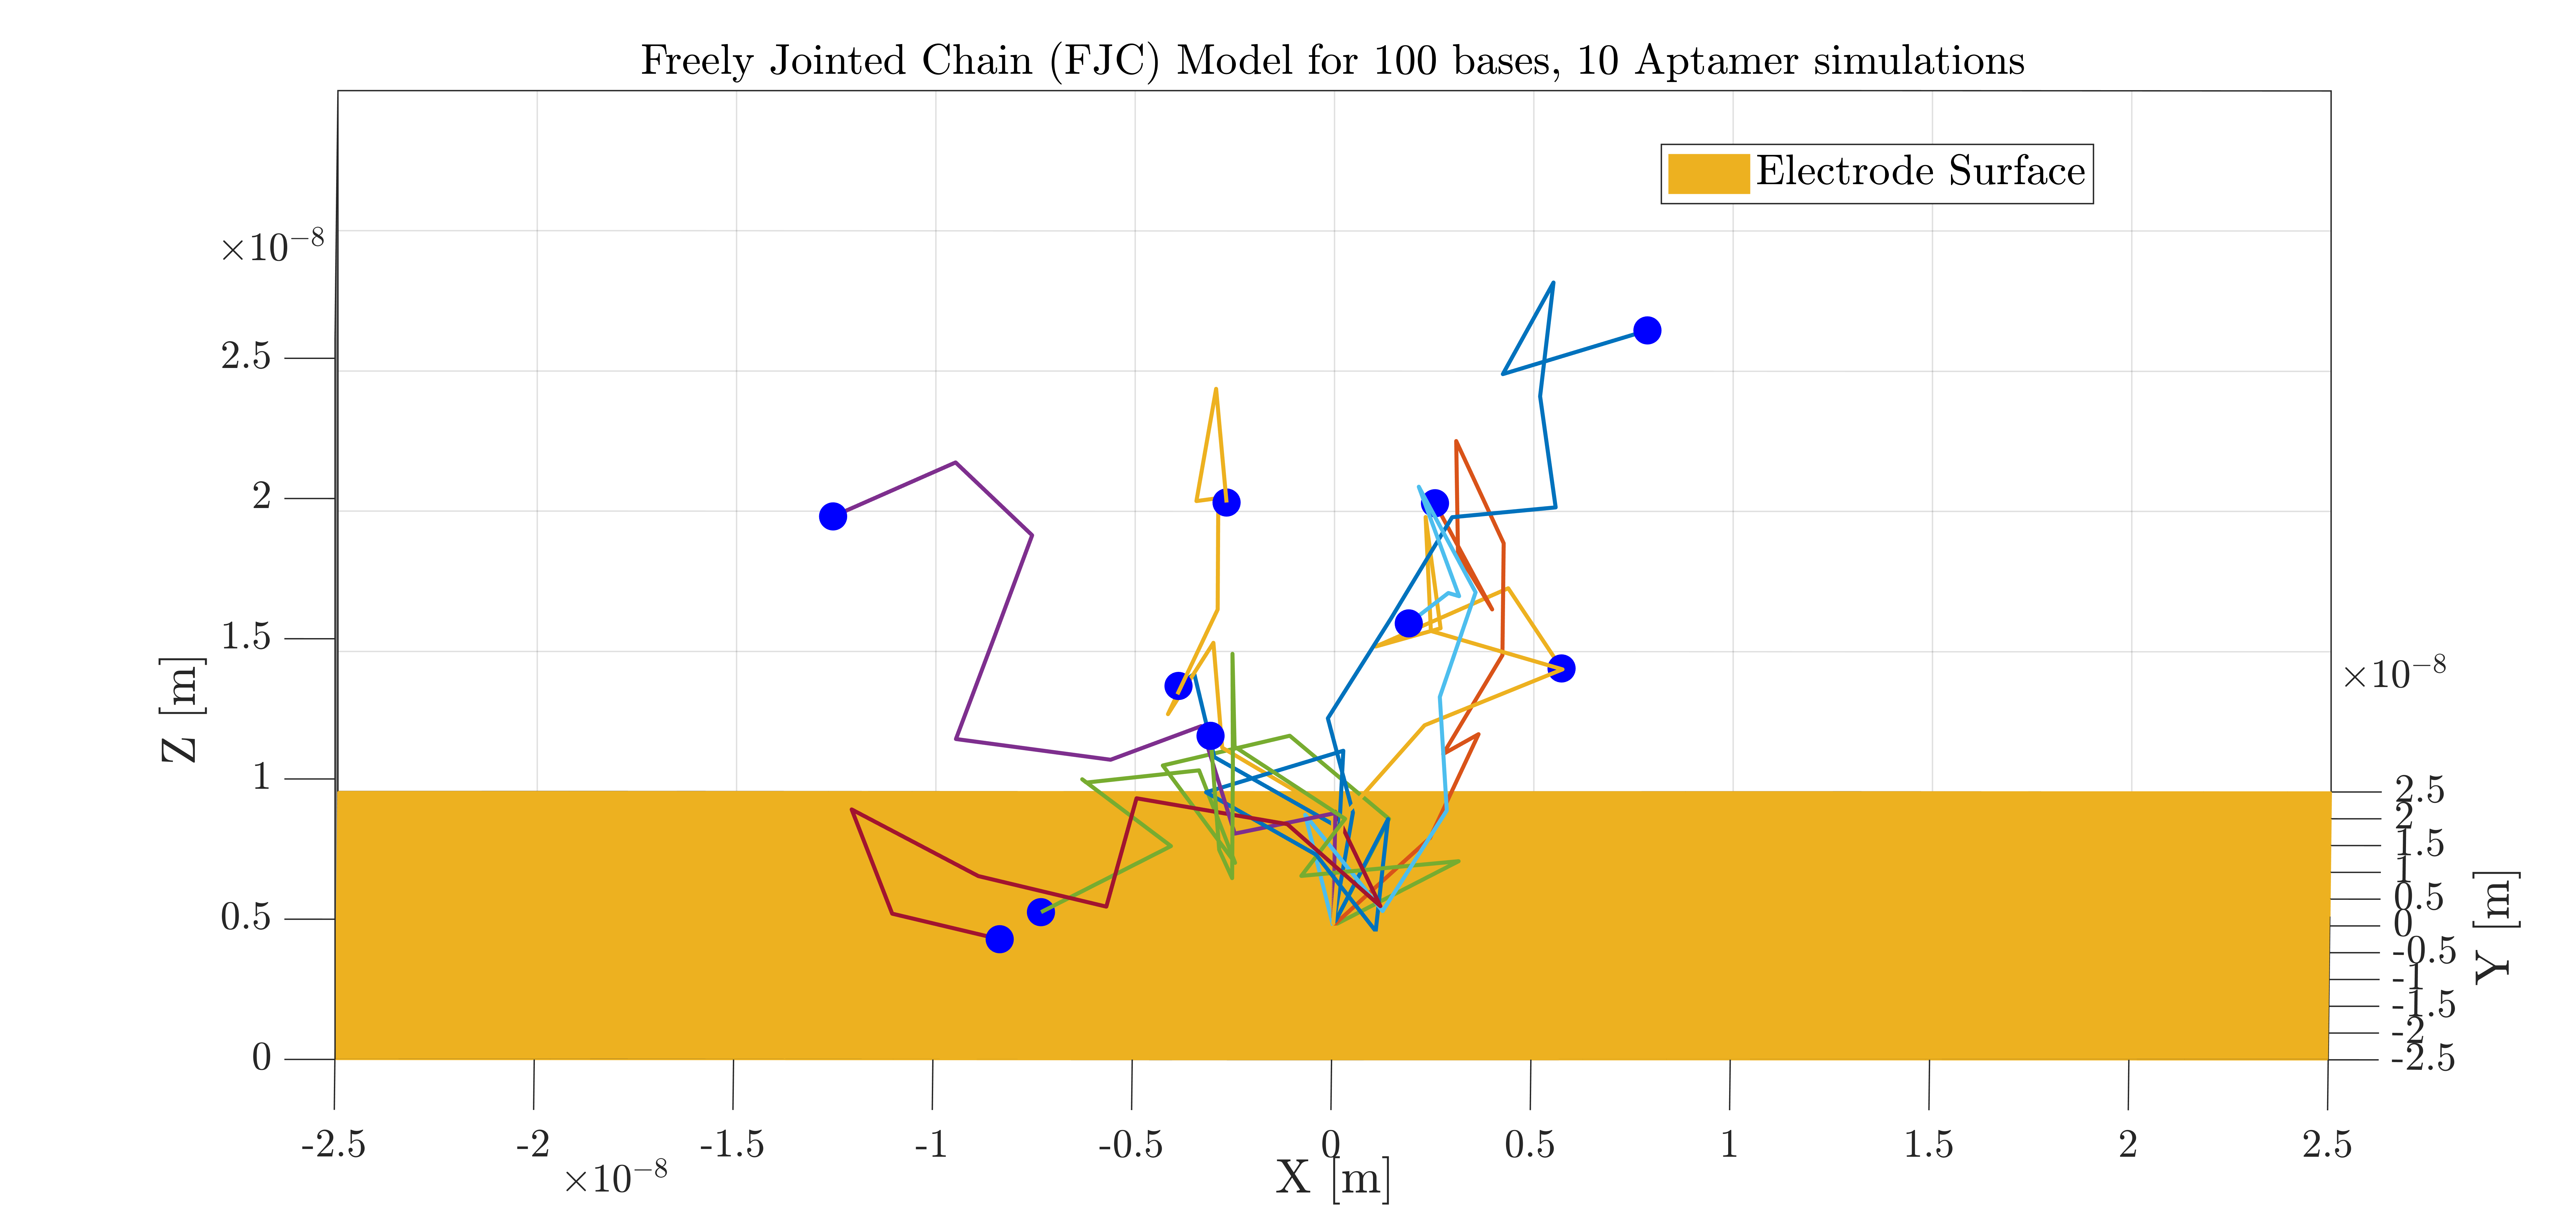
\includegraphics[width = 0.5\textwidth]{img/DNA_100_base_simulation_v1.png}
    \caption{Example plot of 10 random walk simulations for 100 bases with Kuhn length segements (b = 2$\zeta$, where $\zeta$ is the persistence length of the DNA}
    \label{Apt_sim}
\end{figure}
\begin{figure}[H]
    \centering
    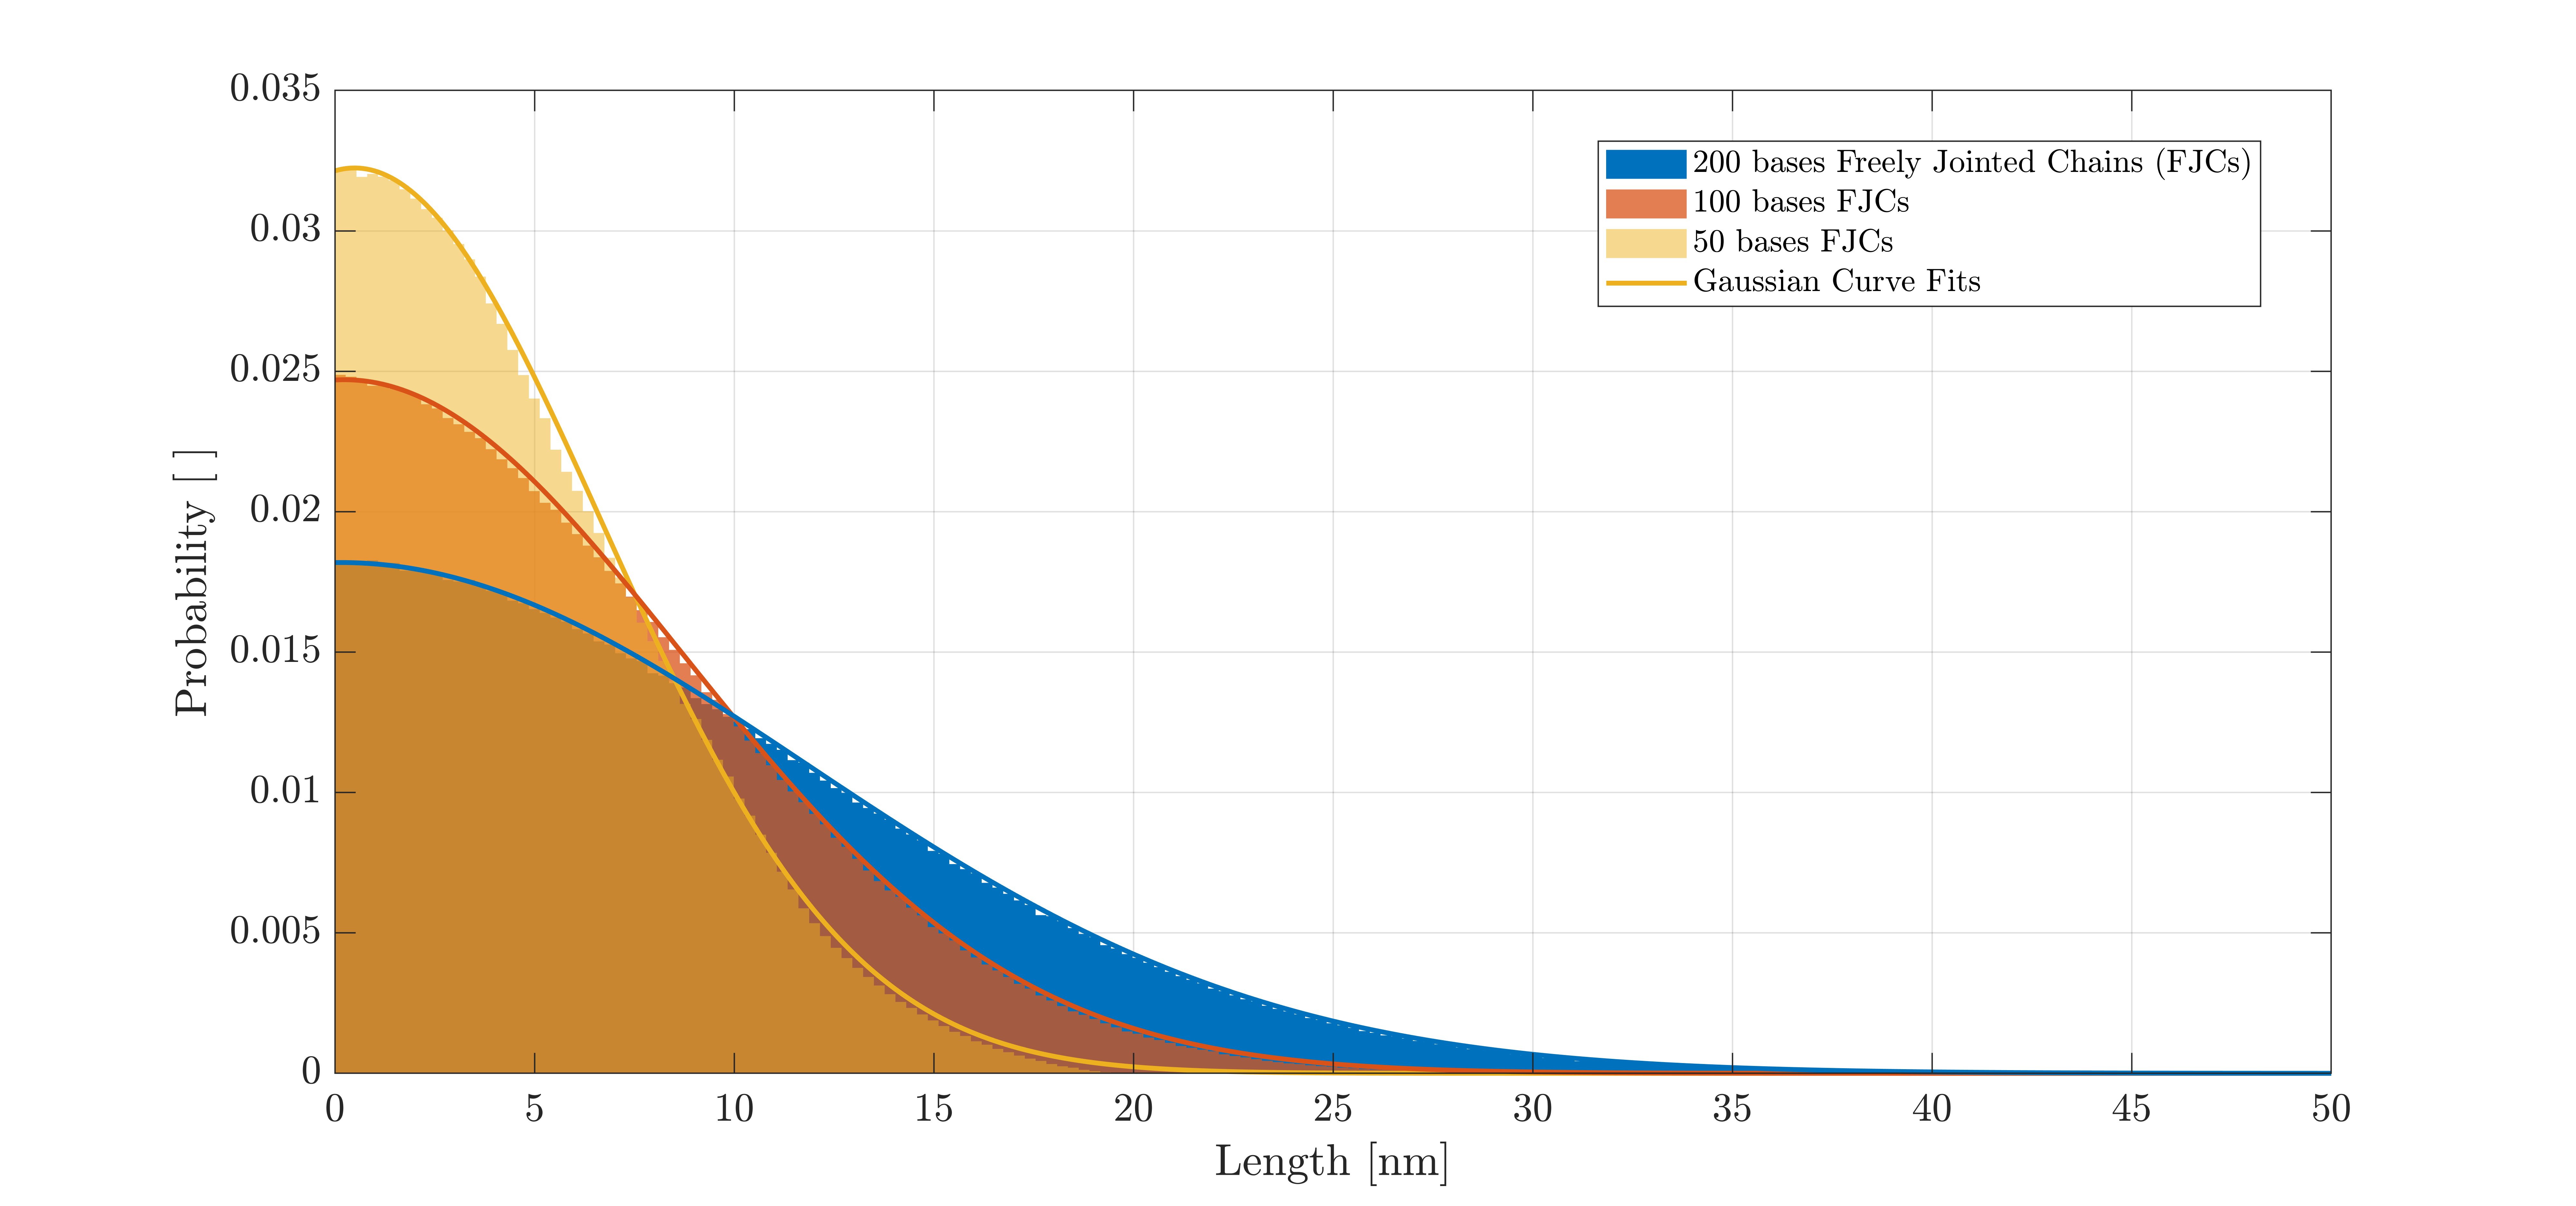
\includegraphics[width = 0.5\textwidth]{img/length_with_gaussians.png}
    \caption{Length probability distribution for aptamers of 200, 100, and 50 base lengths. Numerically simulated using the freely-jointed chain model. Assume aptamer bounces off electrode surface when z$\leq$0. Probability distribution approaches a half-gaussian distribution. Gaussian fits overlayed, with parameters shown in table 1}
    \label{L_dist}
\end{figure}



\newpage
\section{Results}

%===================================================================
\subsection{Nitrite Investigations}

\subsubsection{Reusable gold electrode in PBS Solution}
\begin{figure}[H]
    \centering
    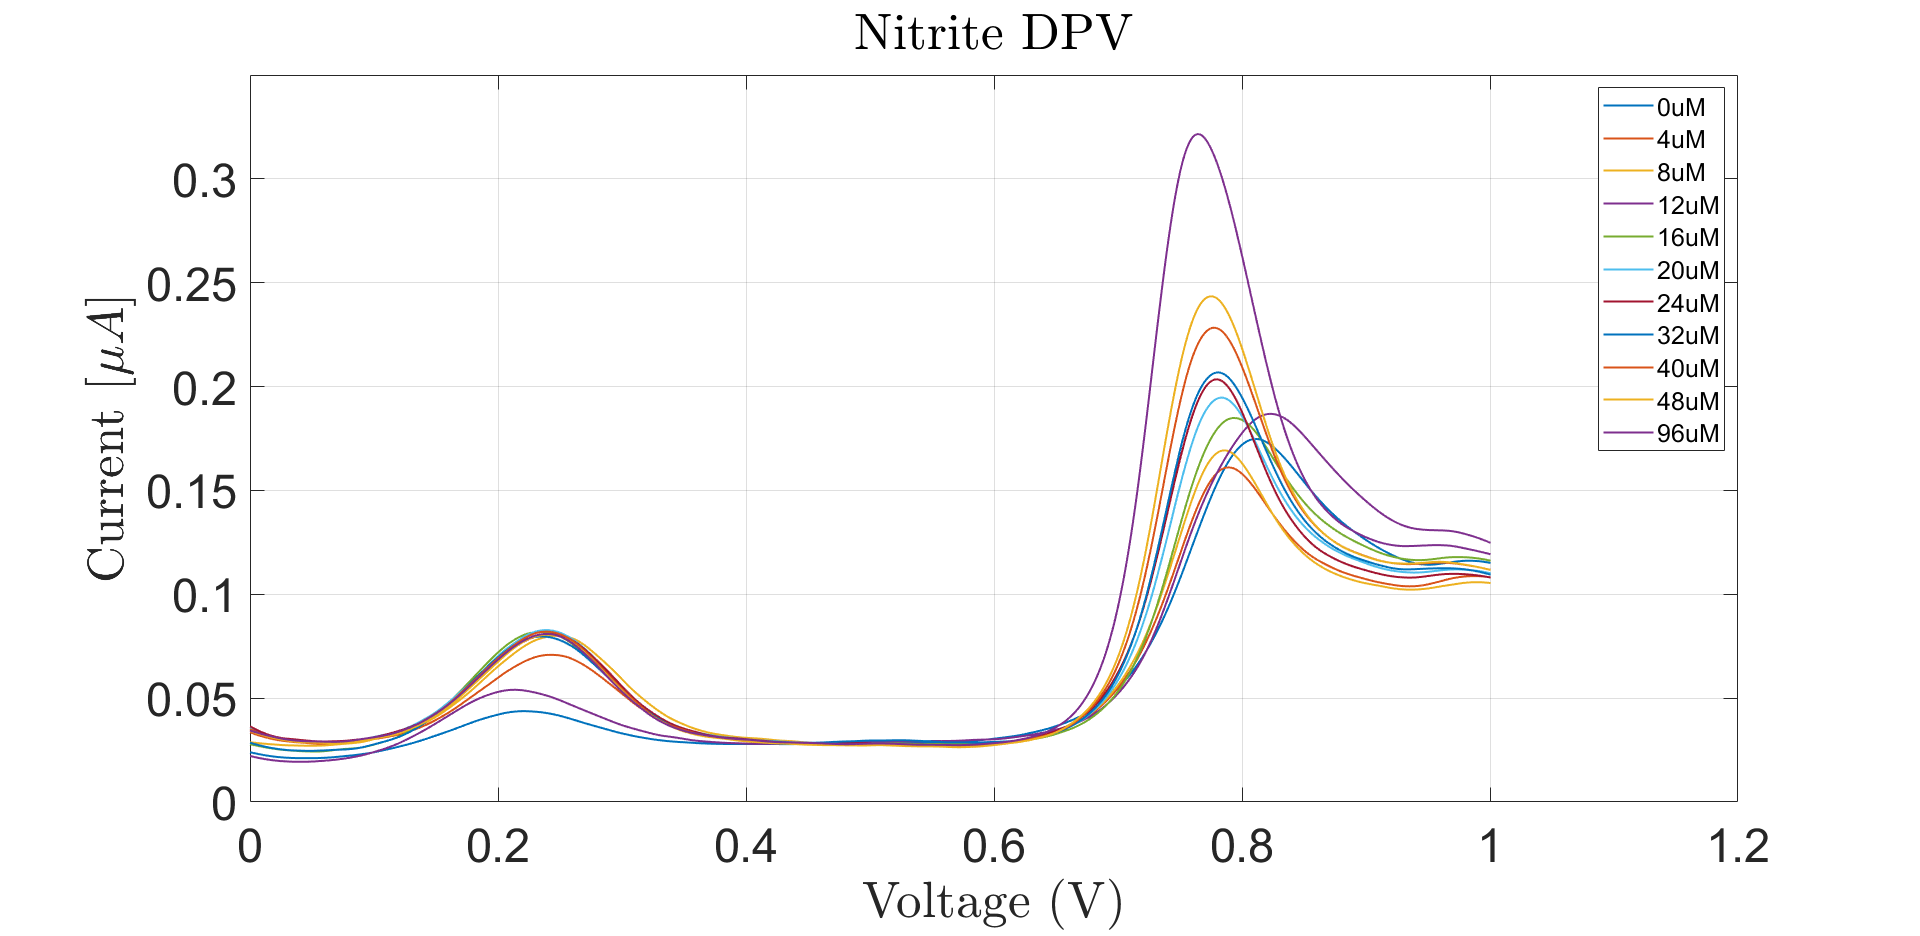
\includegraphics[width = 0.5\textwidth]{img/nitrite clean reus.png}
    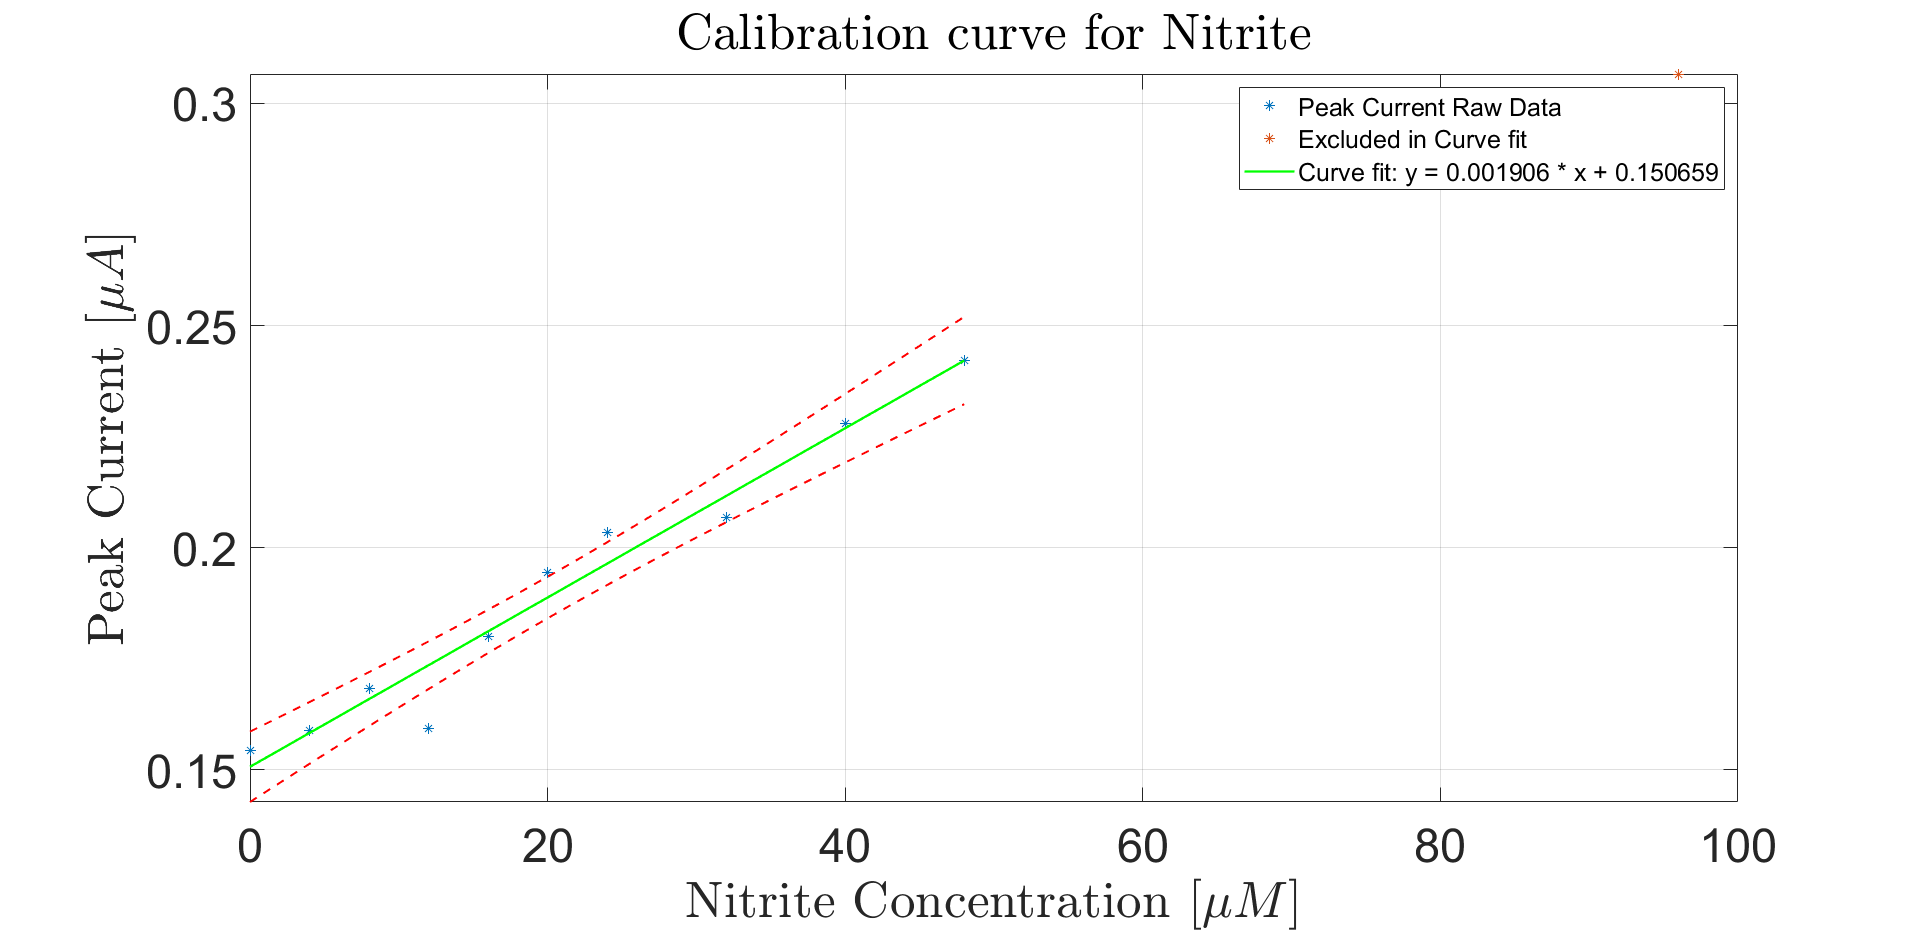
\includegraphics[width = 0.5\textwidth]{img/nitrite clean reus calibration.PNG}
     \caption{Voltammetry and calibration curve of nitrite in PBS - Reusable gold electrode. Calibration curve with regression line and 95\% CI} 
    \label{fig:nitrite_result_1}
\end{figure}

\subsubsection{Reusable gold electrode in PBS Solution and albumin}
\begin{figure}[H]
    \centering
    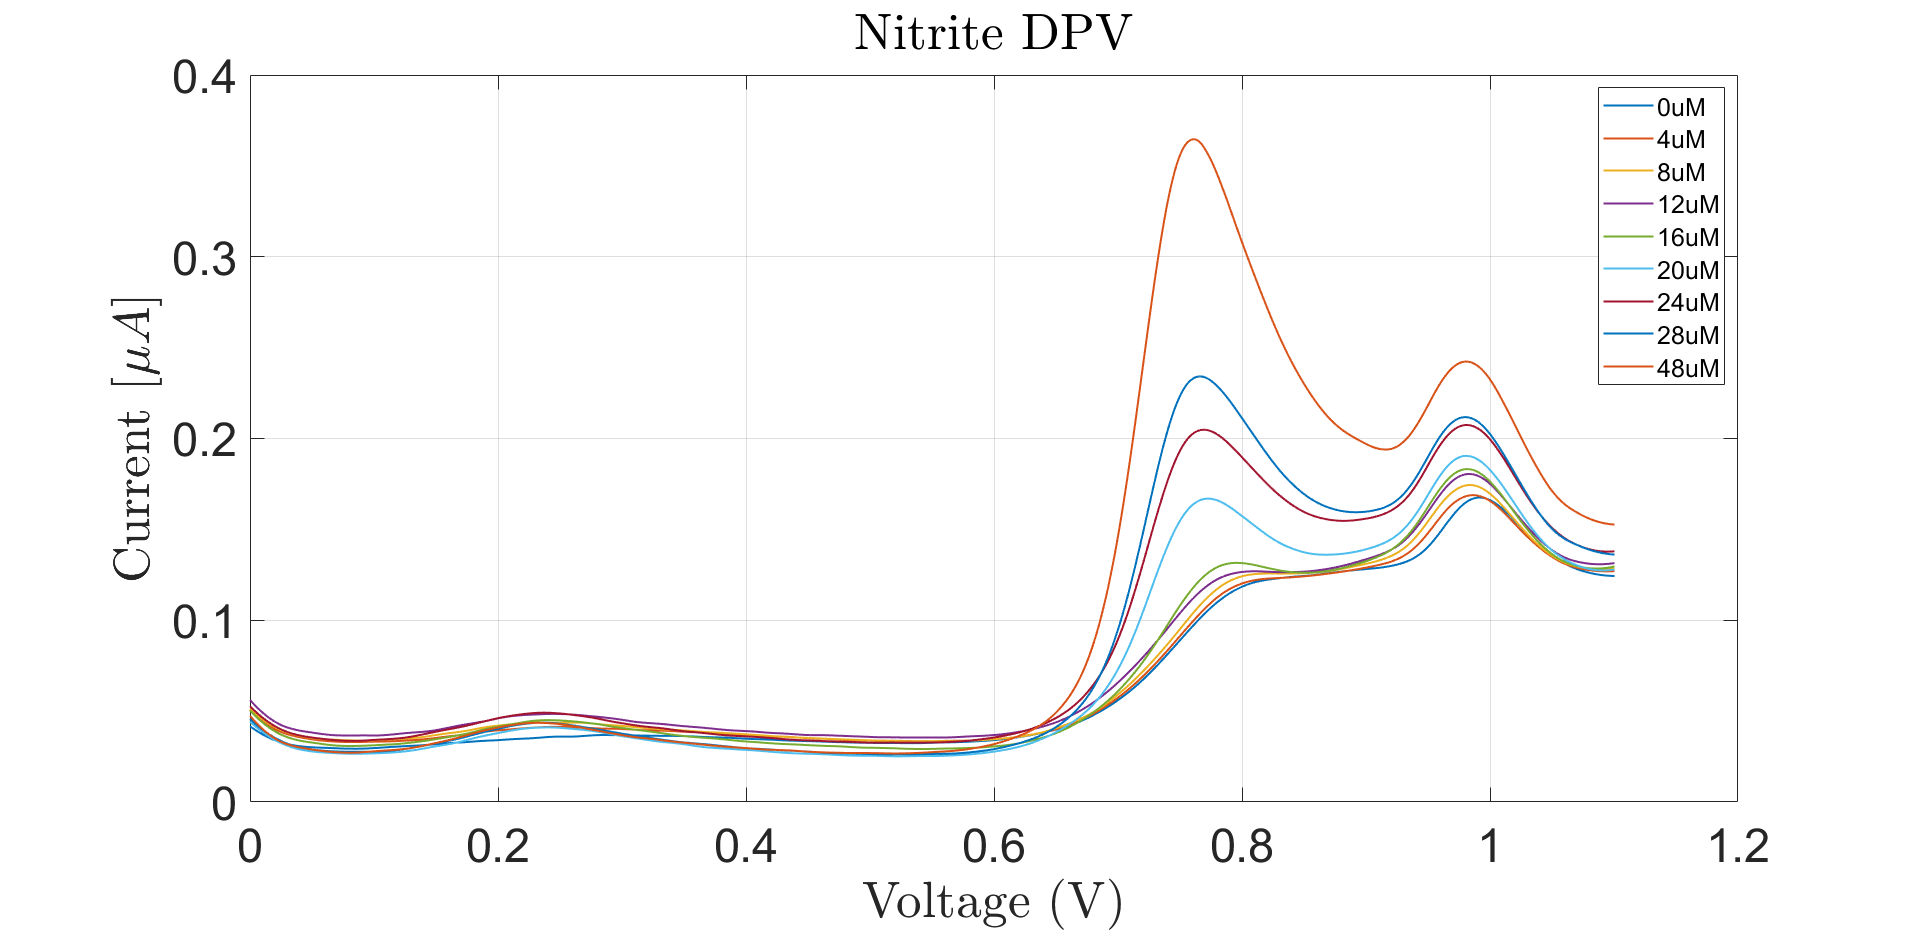
\includegraphics[width = 0.5\textwidth]{img/albumin reus.png}
    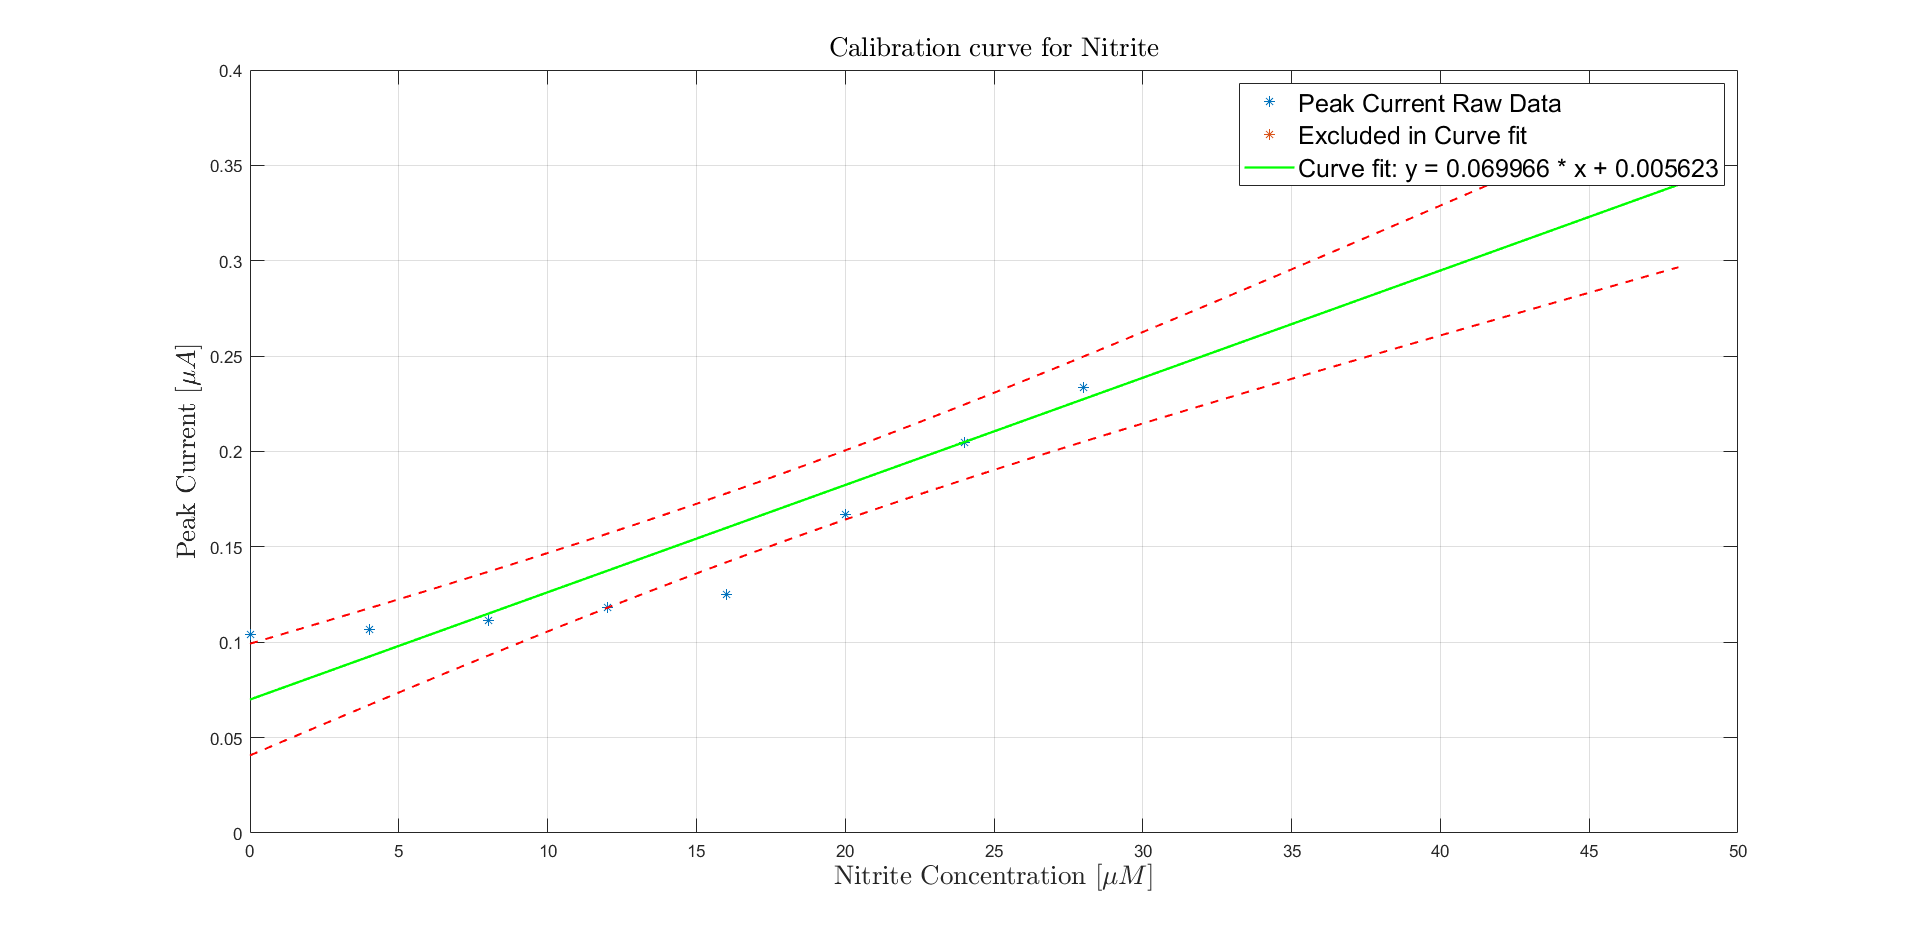
\includegraphics[width = 0.5\textwidth]{img/albumin reus calibration.png}
    \caption{Voltammetry and calibration curve of nitrite in PBS and 5.2 g/L albumin - Reusable gold electrode. Calibration curve with regression line and 95\% CI} 
    \label{fig:nitrite_result_2}
\end{figure}

\subsubsection{Disposable gold electrode in PBS Solution}
\begin{figure}[H]
    \centering
    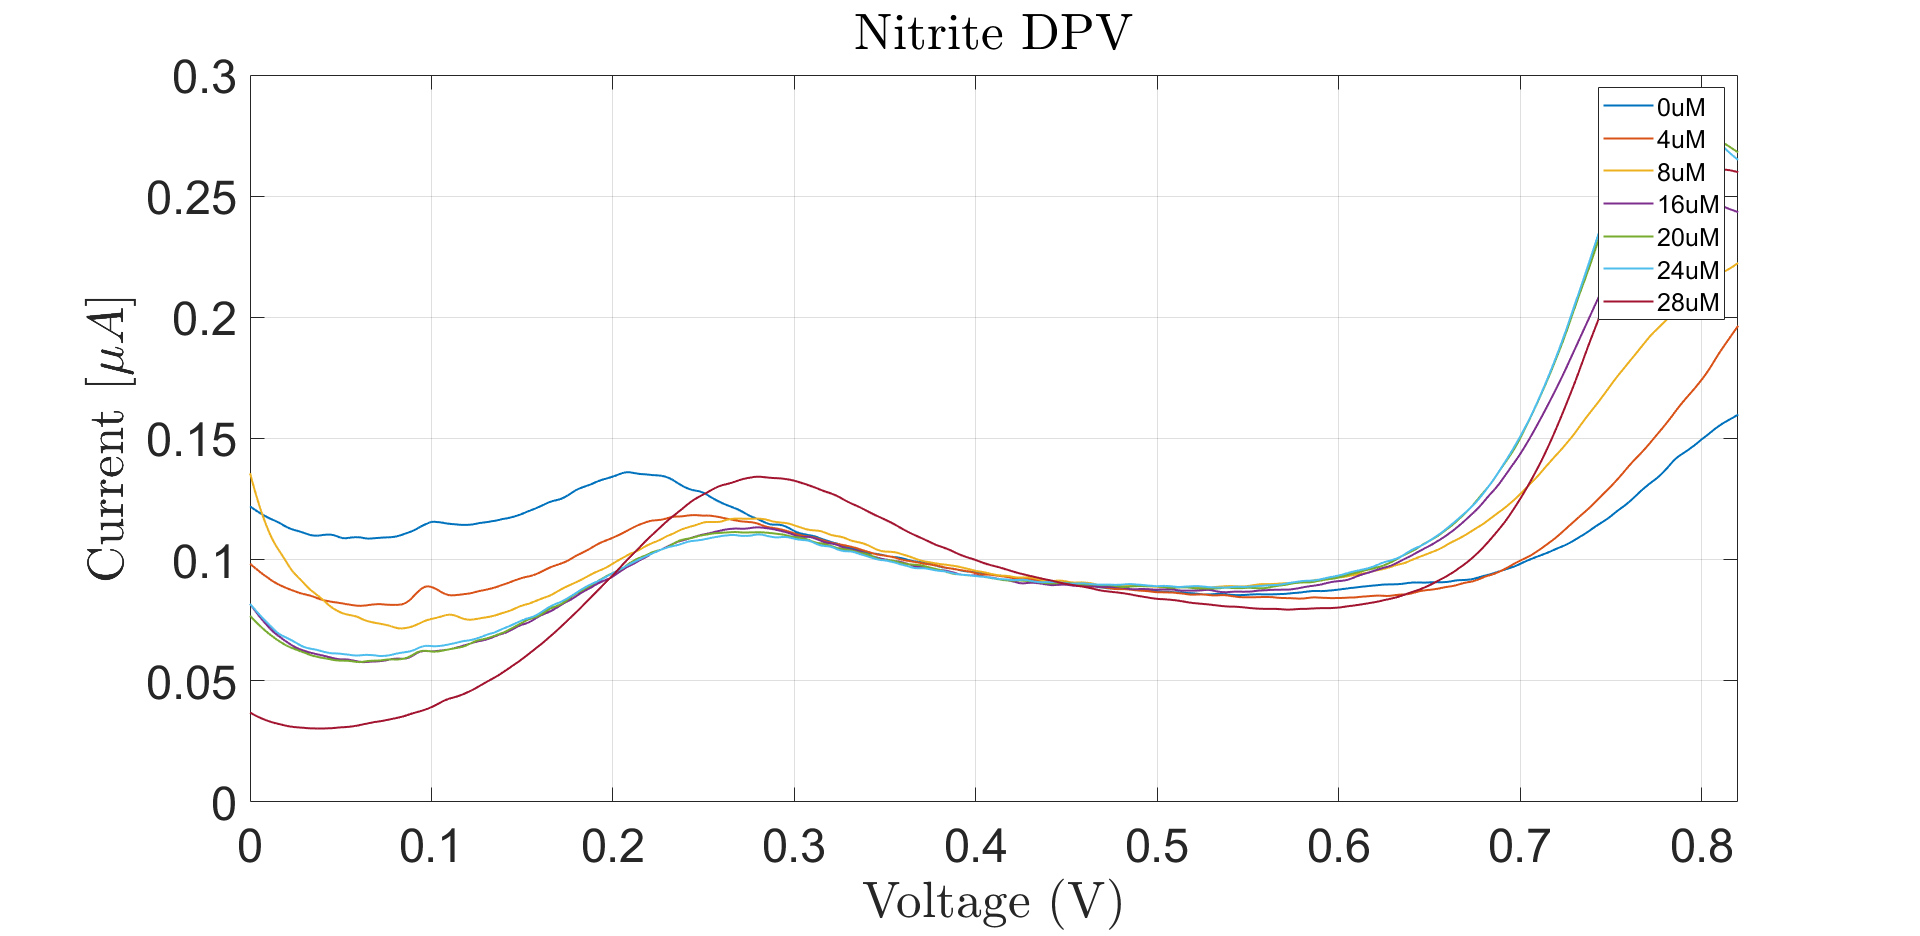
\includegraphics[width = 0.5\textwidth]{img/disp clean.png}
    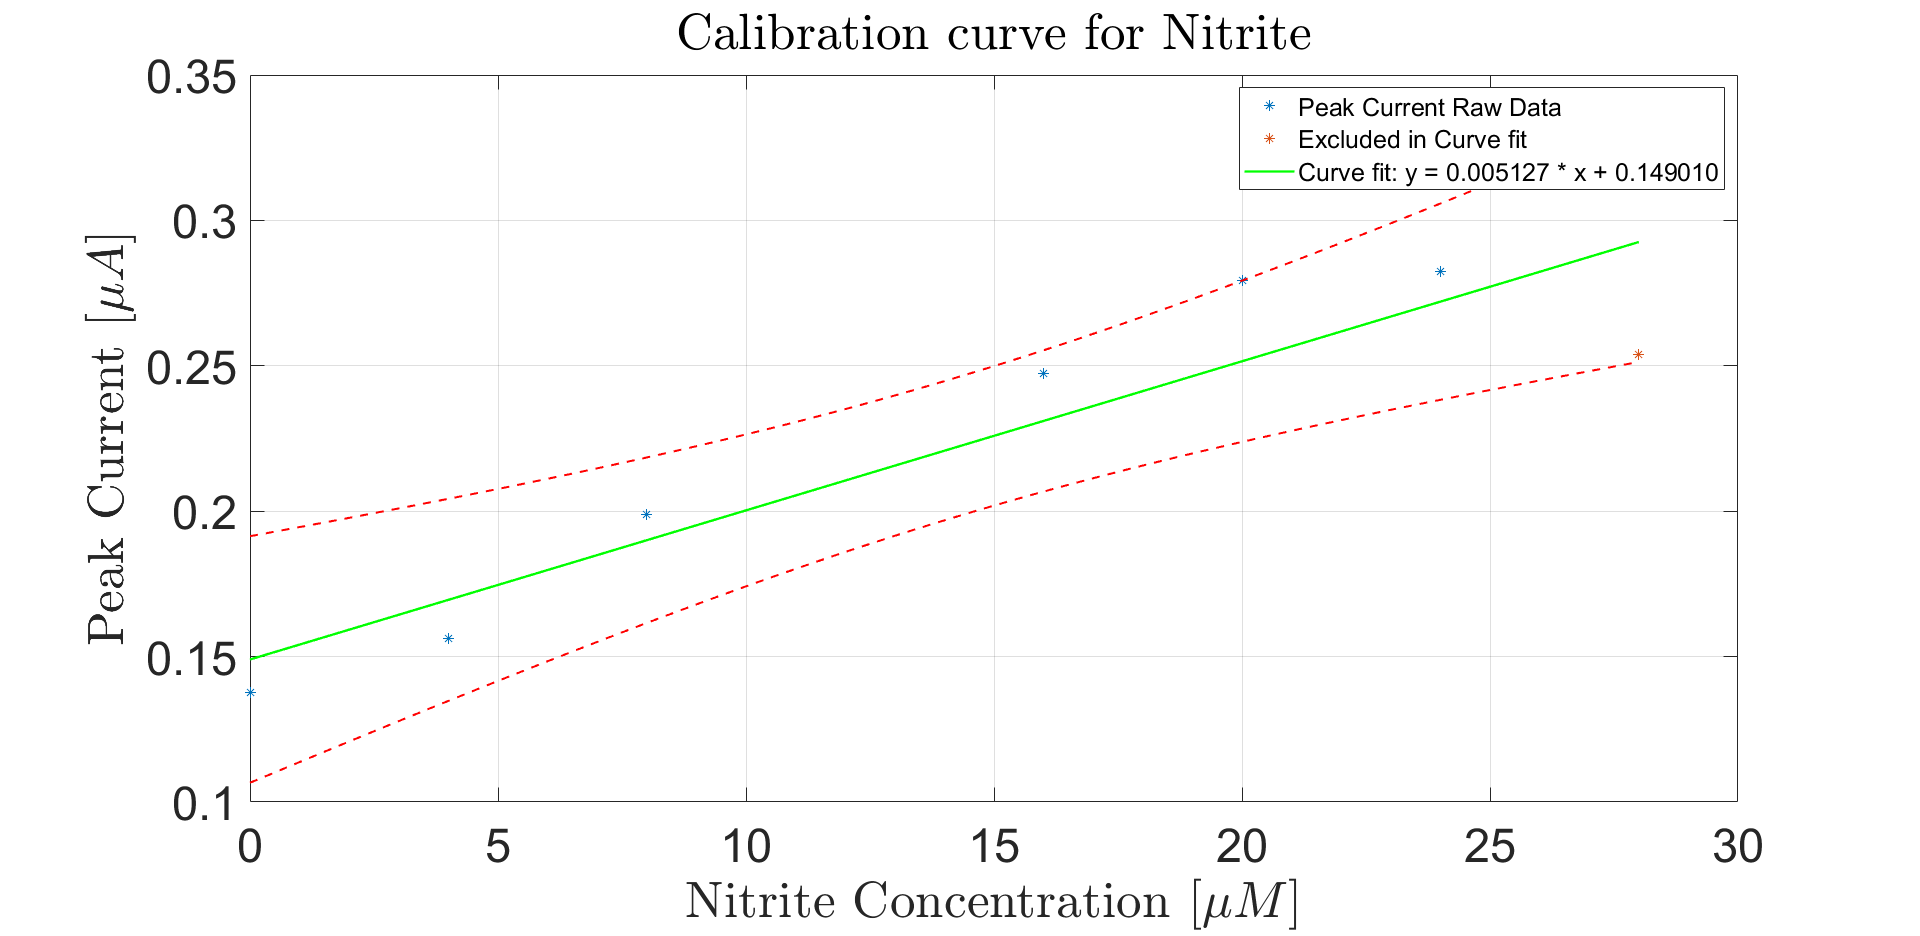
\includegraphics[width = 0.5\textwidth]{img/disp clean calibration.png}
    \caption{Voltammetry and calibration curve of nitrite in PBS - Disposable electrode. Calibration curve with regression line and 95\% CI}
    \label{fig:nitrite_result_3}
\end{figure}

\subsubsection{Disposable gold electrode in PBS Solution and albumin}
\begin{figure}[H]
    \centering
    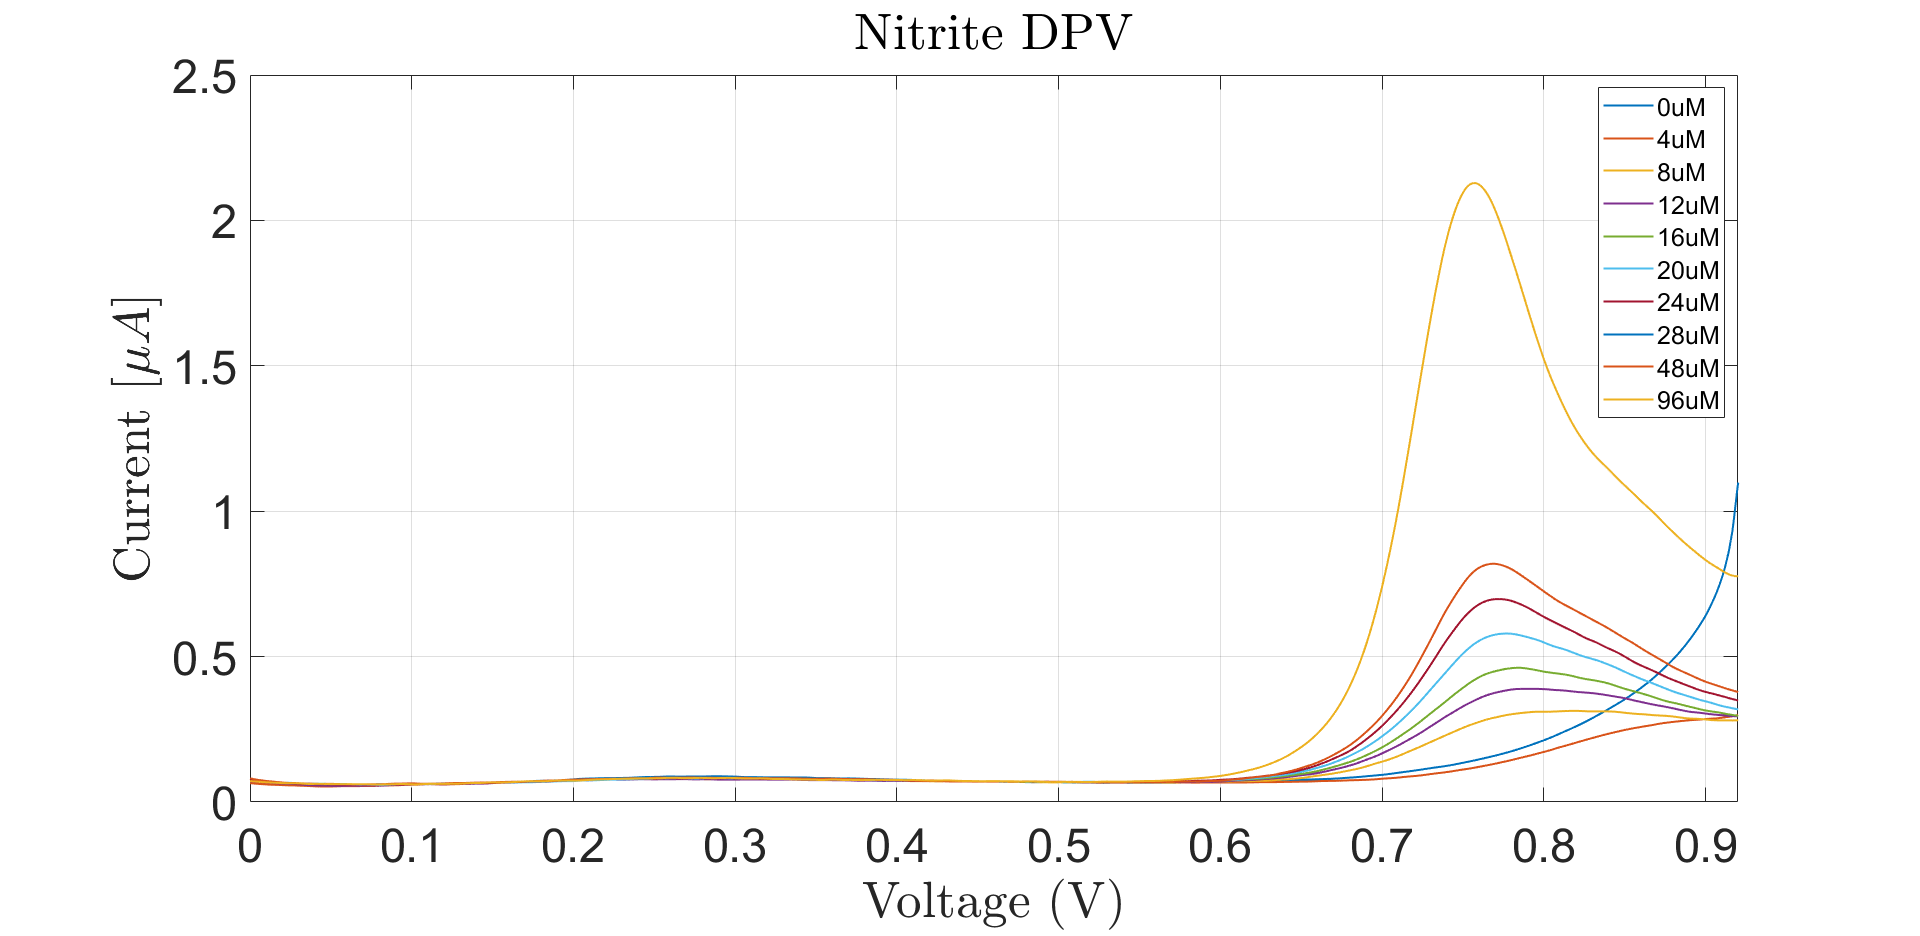
\includegraphics[width = 0.5\textwidth]{img/disp albumin.png} 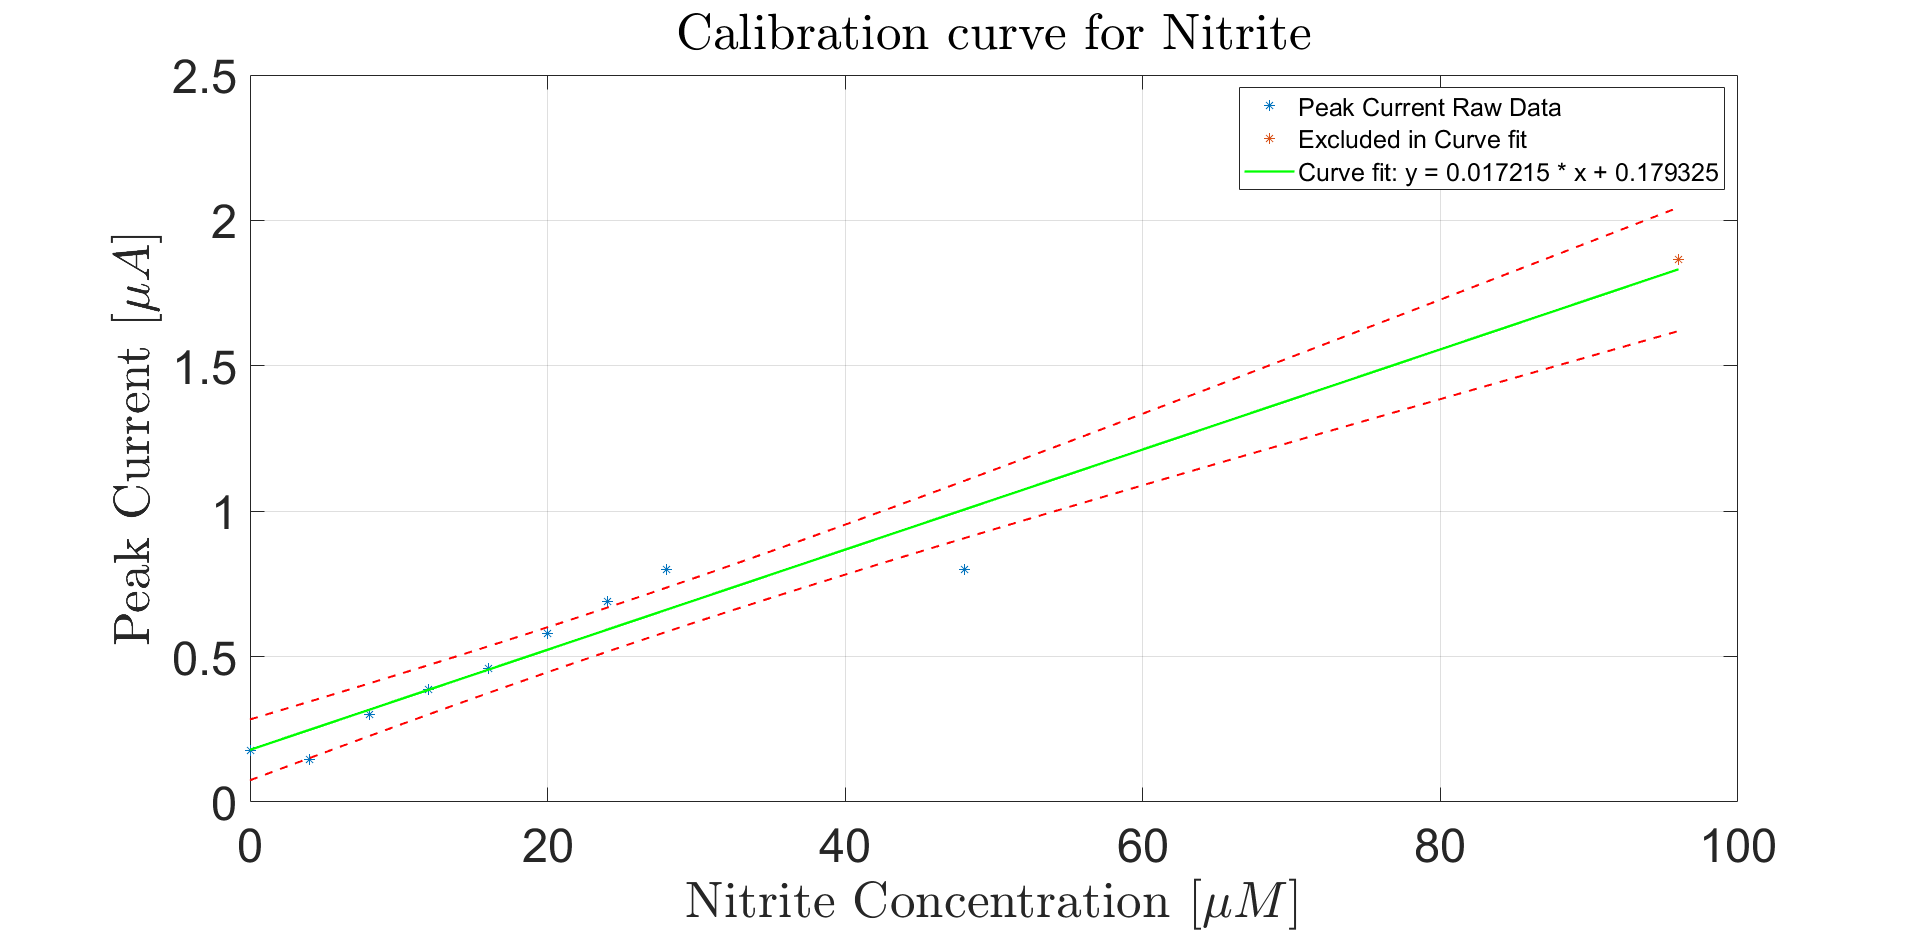
\includegraphics[width = 0.5\textwidth]{img/disp albumin calibration.png}
    \caption{Voltammetry and calibration curve of nitrite in PBS and 5.2 g/L albumin - Disposable electrode. Calibration curve with regression line and 95\% CI}
    \label{fig:nitrite_result_4}
\end{figure}

\subsubsection{Summary of calibration curves}
\begin{figure}[H]
    \centering
    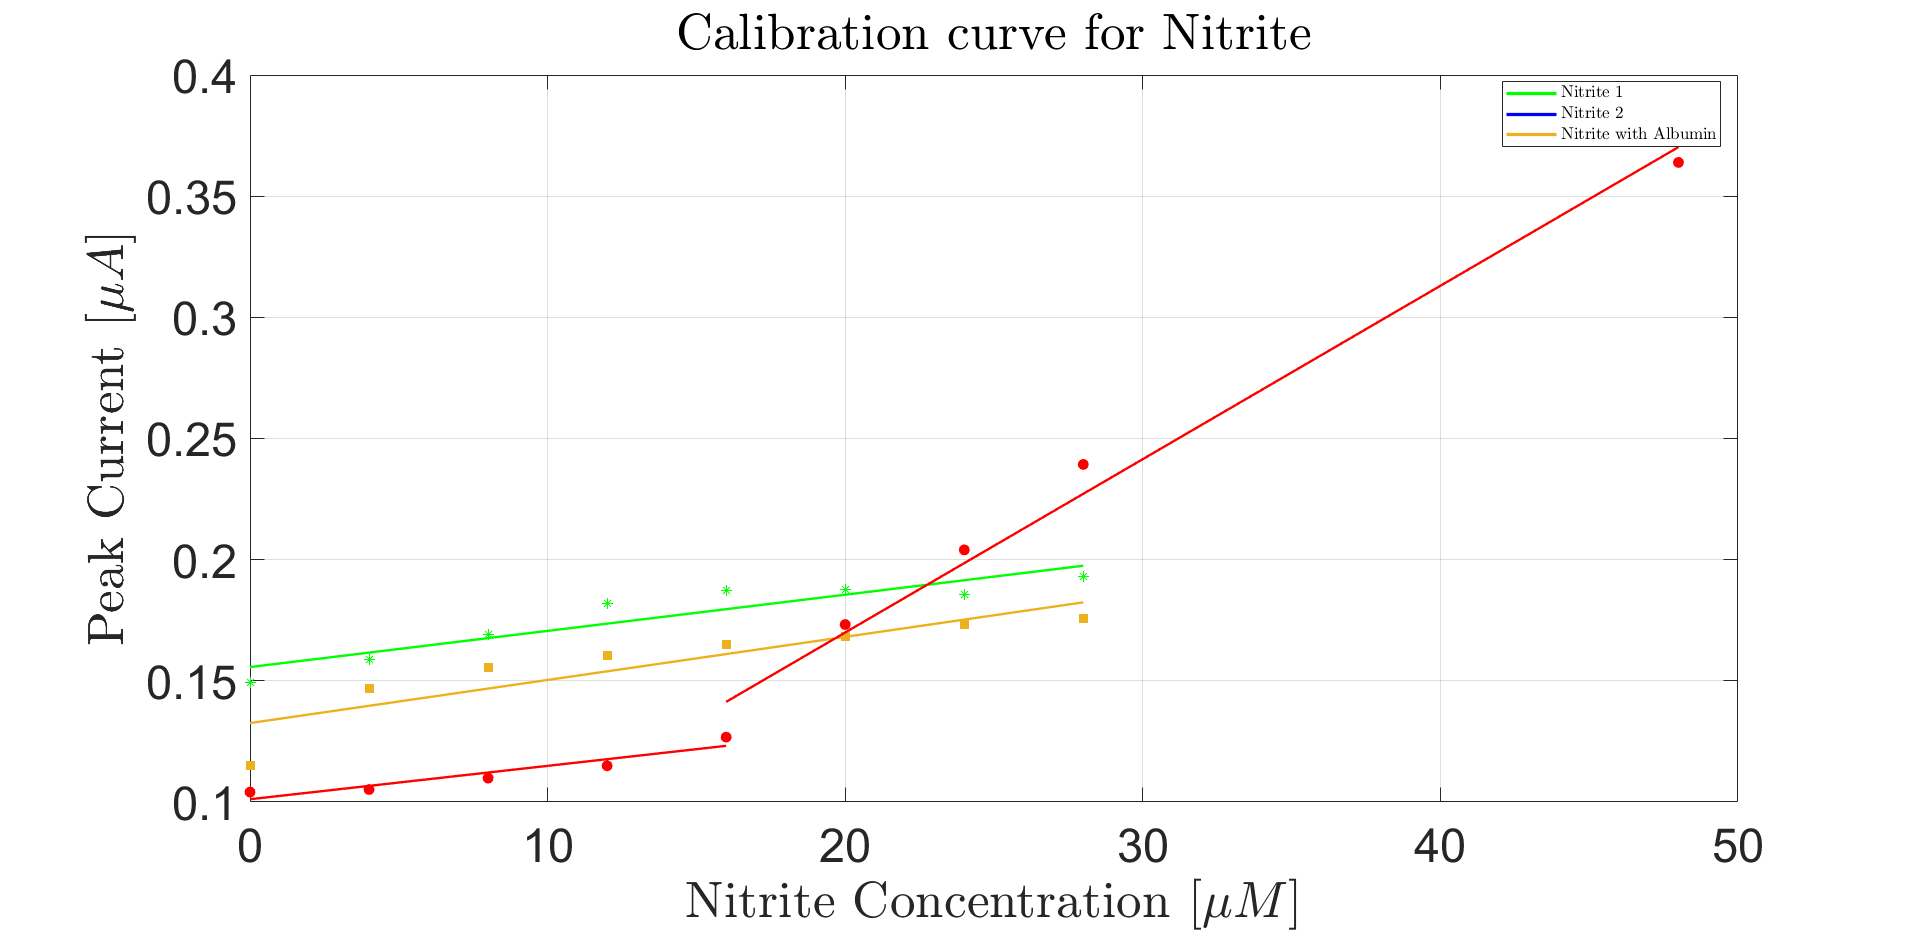
\includegraphics[width = 0.5\textwidth]{img/combinedreus new.png}
    \caption{Combined plot of reusable electrode calibration curve regression lines}
    \label{fig:nitrite_calibration_1}
\end{figure}

\begin{figure}[H]
    \centering
    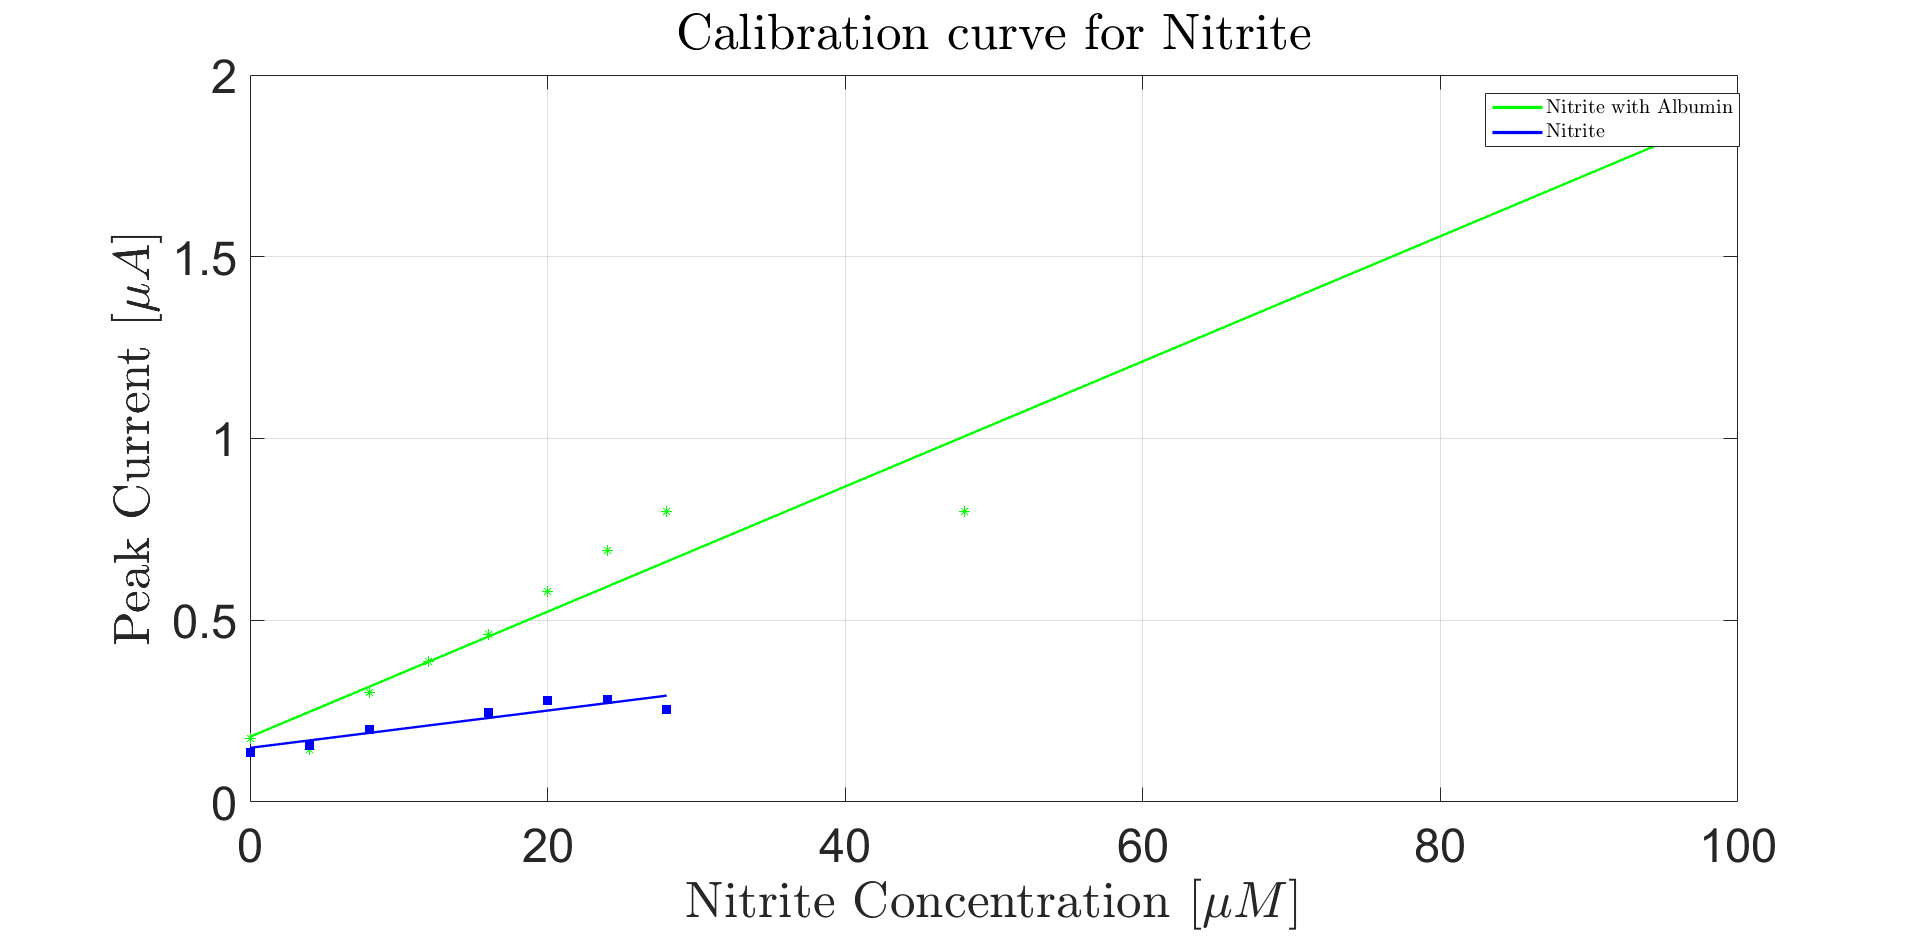
\includegraphics[width = 0.5\textwidth]{img/combined disp.png}
    \caption{Combined plot of disposable electrode calibration curve regression lines}
    \label{fig:nitrite_calibration_2}
\end{figure}

\begin{table}[H]
    \centering
    \begin{tabularx}{0.5\textwidth}{|p{1cm}|p{2.3cm}|c|c|c}\hline
    
    Nitrite & Sensitivity$\pm$SD /n\text{A} $\mu \text{M}^{-1} (s)$ & Intercept $(\mu \text{A})$ & LOD $(\mu \text{M})$ \\ \hline
    
    \textbf{1} & 1.5$\pm$0.5 & 0.156 &1.314  &   \\ \hline
    
    \textbf{2} & 1.9$\pm$.3 & 0.151$\pm$0.008 &  0.543&   \\ \hline
    
    \textbf{3} &1.8$\pm$0.8  &  0.133$\pm$0.5& 1.660 &   \\ \hline
    \end{tabularx}
    \caption {Sensitivity and LOD values for nitrite experiments}
    \end{table}
Current from increasing steps in E were measured and recorded. These were used to plot voltammograms with current as a function of voltage. Current drift was corrected and smoothed. Current of the highest peaks, between 0.7 and 0.8V in all graphs were recorded. Results obtained from each experiment are shown above.  A linear regression line with 95\% confidence intervals was constructed as shown in \autoref{fig:nitrite_result_1}, \ref{fig:nitrite_result_2}, \ref{fig:nitrite_result_3} and \ref{fig:nitrite_result_4}. Regression lines were then plotted alongside each other to compare gradients and SD between experiments, shown in \autoref{fig:nitrite_calibration_1} and \ref{fig:nitrite_calibration_2}.\\\\
DPV for measuring nitrite concentration using reusable gold electrodes in PBS was performed three times, returning similar traces each time (\autoref{fig:nitrite_result_1}). Performing linear regression produced curves with similar gradient, with no significant difference due to overlapping standard deviations.\\\\
Code used for plotting and processing collected data is documented in \autoref{app:nitrite_code}.
%=========================================================================================
\subsection{Hydrogen Peroxide Investigations}
Upon completing four cyclic voltammetry scans, the following voltage-current plot was obtained by taking the data from the last stable scan. A peak voltage at 0.209V and a trough voltage at -0.204V were observed when the applied sweep current reached 0.024mA and -0.321mA respectively, corresponding to the oxidation and reduction processes of PB. This process is an essential validation of the presence of PB in the experiment setup.  
\begin{figure}[H]
    \centering
    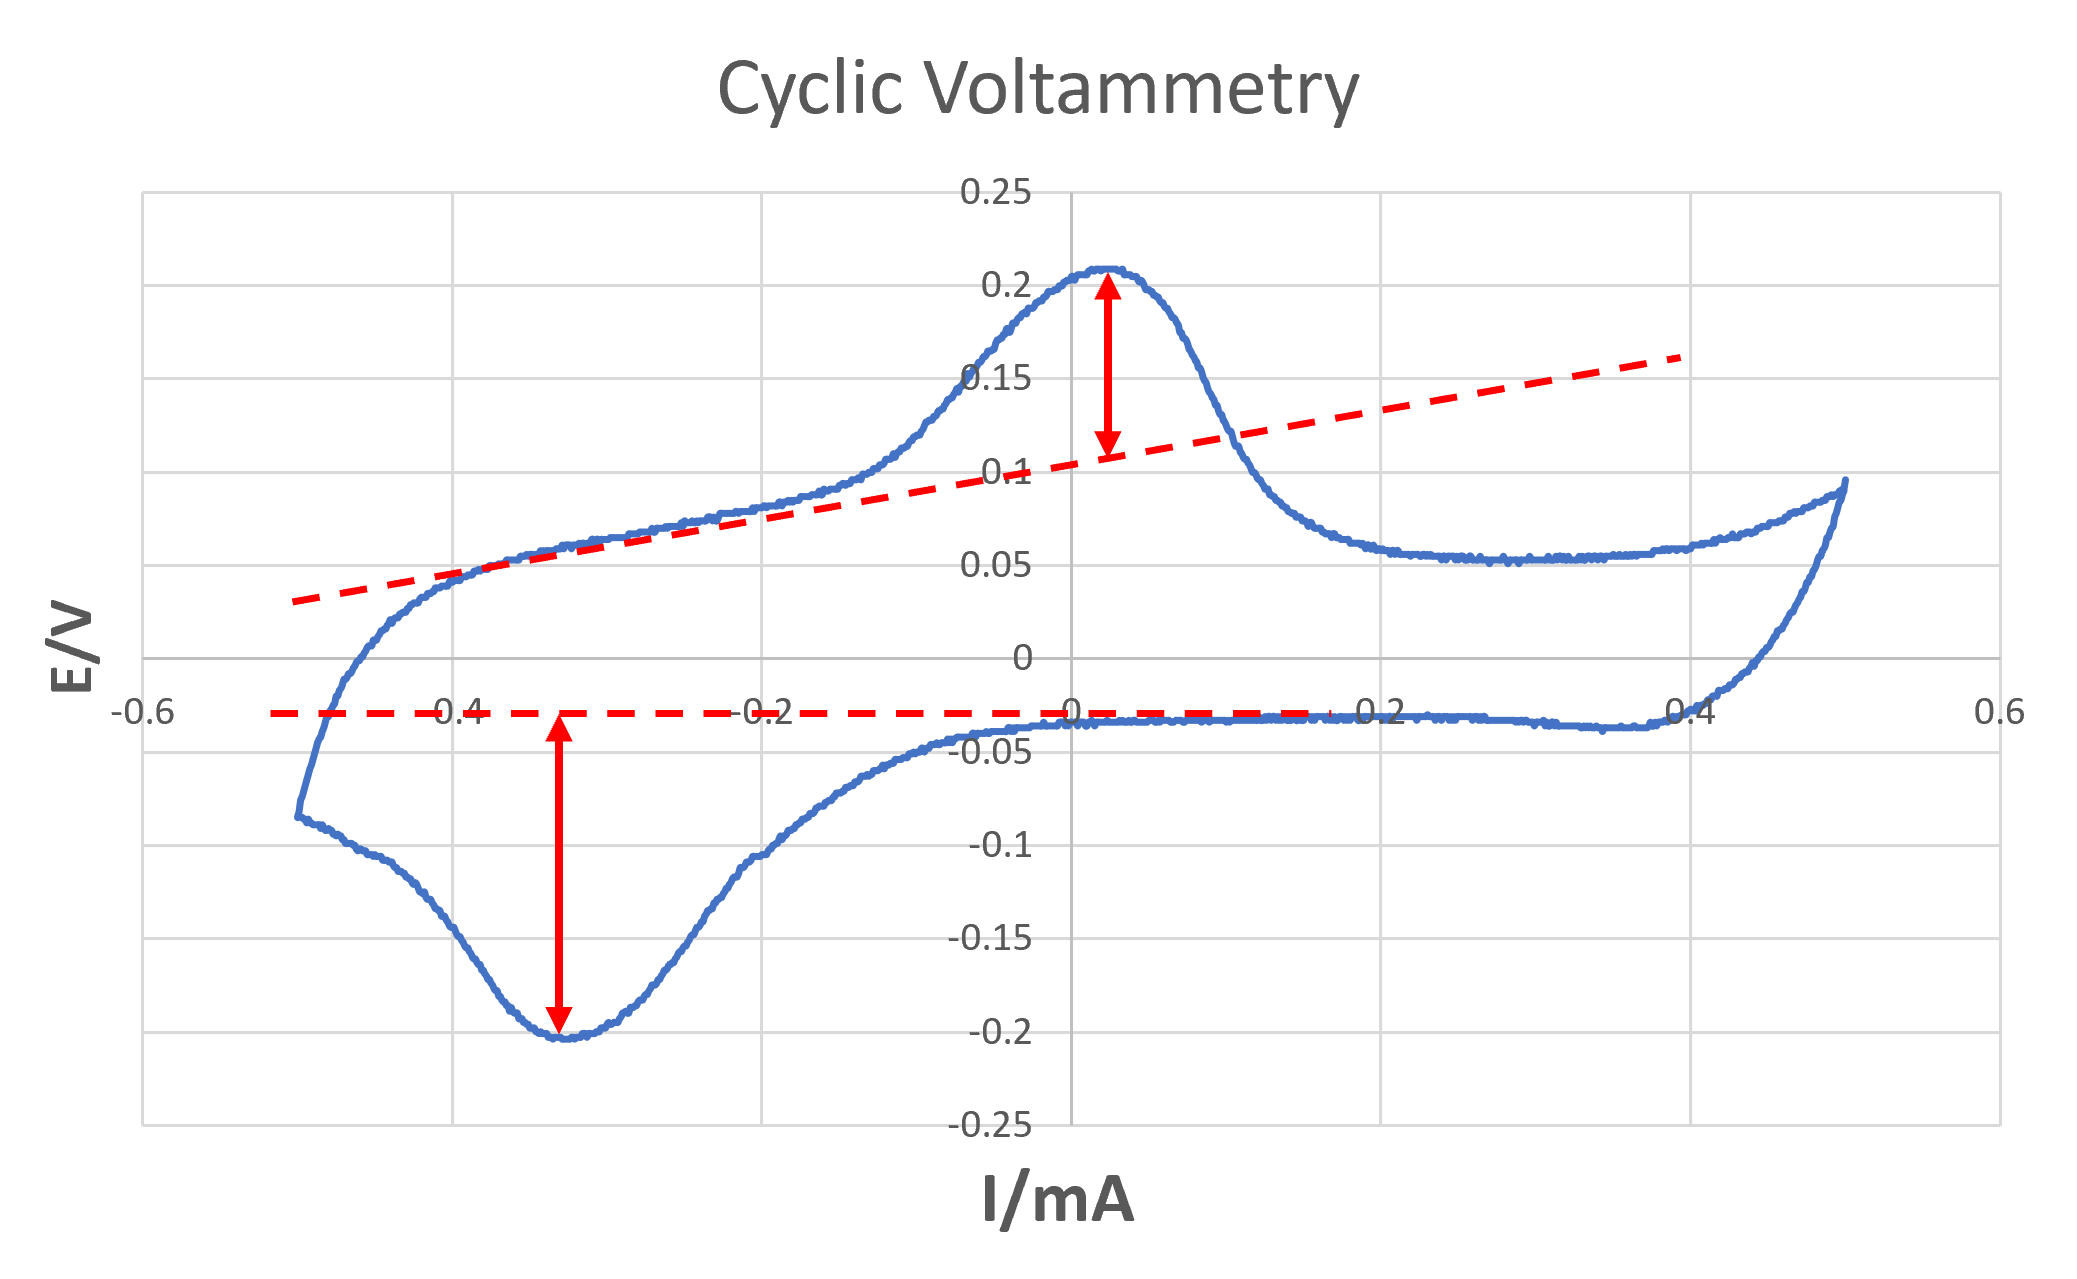
\includegraphics[width=.5\textwidth]{img/h2o2_cv.png}
    \caption{Cyclic voltammetry result}
    \label{fig:h2o2_cv}
\end{figure}
\noindent Chrono amperometry was performed following the cyclic voltammetry scan. The obtained results are shown in \autoref{fig:h2o2_amp}: hydrogen peroxide concentration ranged from 0 to M where stable current decreased with increased concentrations.
\begin{figure}[H]
    \centering
    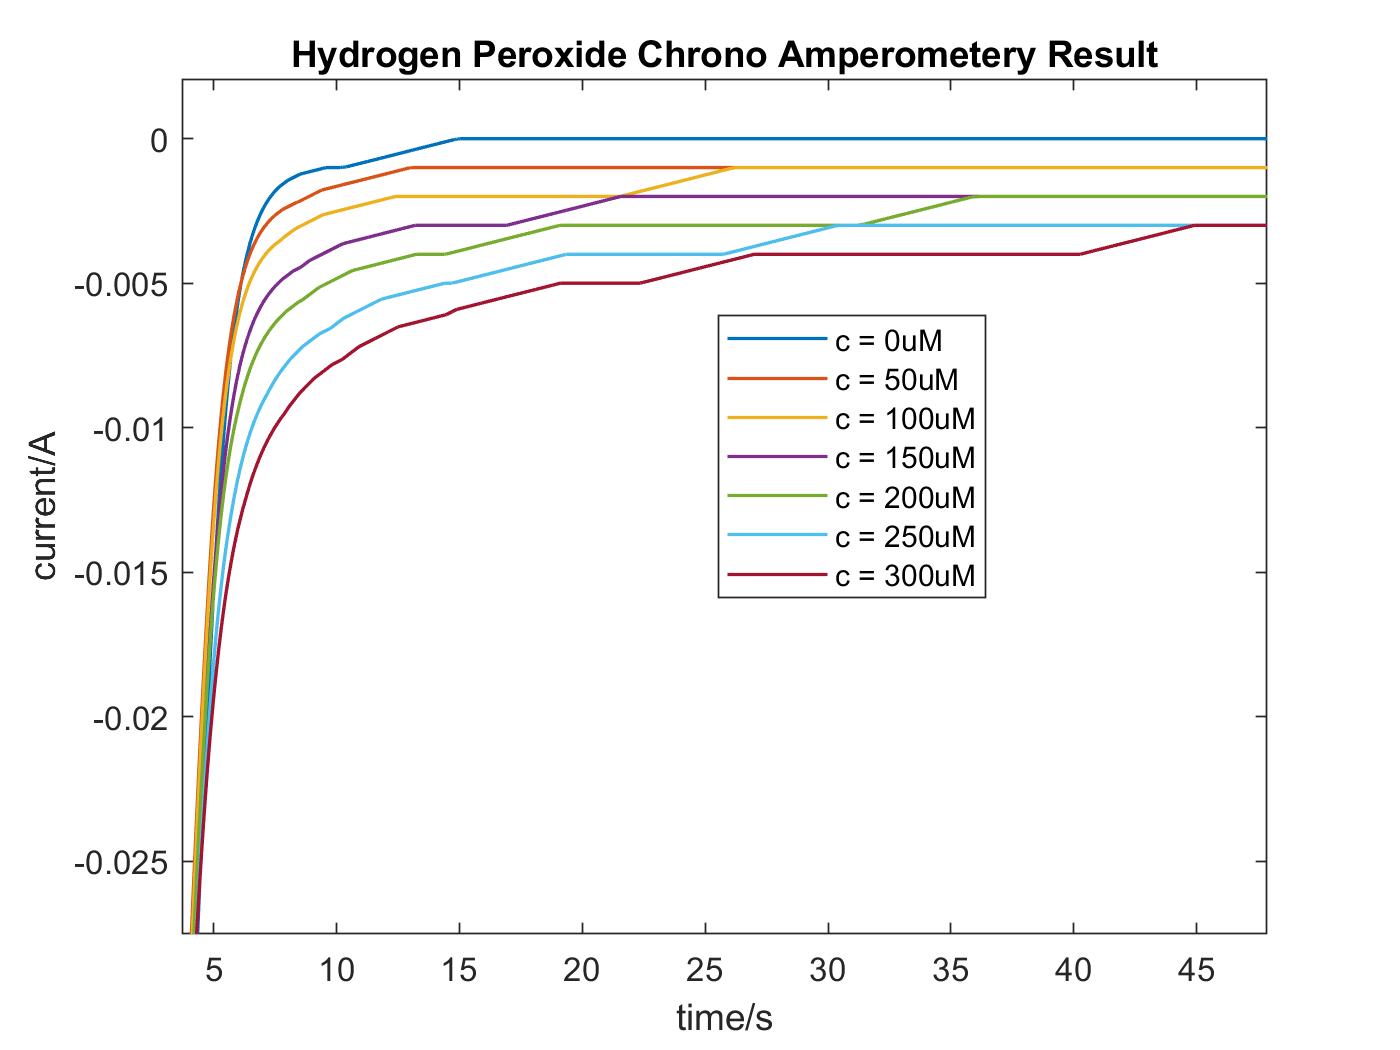
\includegraphics[width=.5\textwidth]{img/h2o2_amp.png}
    \caption{Cyclic voltammetry result}
    \label{fig:h2o2_amp}
\end{figure}
\noindent Coulometry serves as a powerful tool to amplify the current signal and reduce the noise through integrating the amperometry current data with respect to time \cite{Anson1966}. An improved Anson's equation with the consideration of edge-effect \cite{Flanagan1973} has been implemented to validate the experimental concentrations adopted in the electrode calibration curve, a detailed explanation and realisation of coulometry is shown in \autoref{app:h2o2_coulometry}. The result of coulometry is shown in \autoref{fig:h2o2_col} - the coulometry charge under each experimental concentration was plotted against the edge-corrected time, $(\sqrt{t}+\frac{1.92\sqrt{D}}{r}t)$ where $t$ is the sampling time over 180s. For each curve, a non-linear region was observed in the beginning, corresponding to the non-faradic charge due to double-layer charging and Prussian bule reduction. Following that, a major linear region appears almost immediately, indicating the charge transfer as the result of hydrogen peroxide reduction.
\begin{figure}[H]
    \centering
    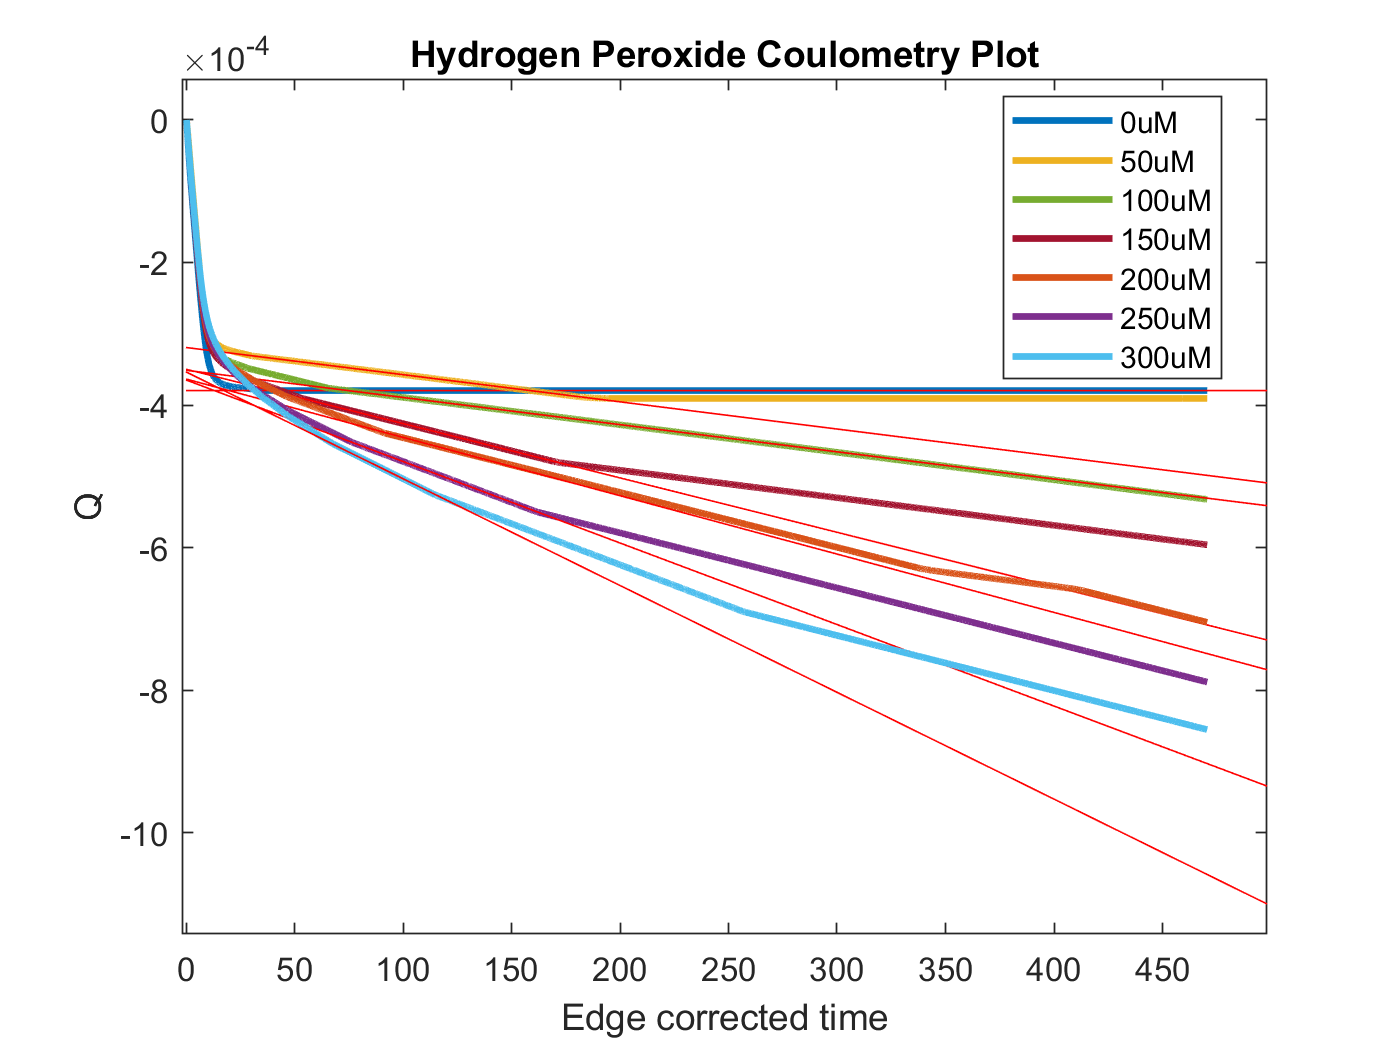
\includegraphics[width=.5\textwidth]{img/h2o2_coulometry.png}
    \caption{coulometry result}
    \label{fig:h2o2_col}
\end{figure}\vspace{-.8cm}
\noindent To perform curve fitting, 500 current and time data points in the linear region were selected from the coulometry curves for each concentration. The gradients of each linear-fitted line were reported in \autoref{tab:h2o2_col_res}, hence we calculated the theoretical concentrations based on the relation in \autoref{eqn:improved_anson}. Comparisons between the theoretical and experimental concentrations were then performed.
\begin{table}[H]
    \centering
    \begin{tabularx}{.45\textwidth}{|p{.12\textwidth}|p{.13\textwidth}|p{.126\textwidth}|}\hline
        Experimental concentration (uM) & Gradient of linear fitting line & Theoretical concentration (uM)  \\ \hline
        0   & -1.216e-19 $\pm$ 0 & 2.39e-19\\ \hline
        50  & -3.814e-07 $\pm$ 0 & 84.30\\ \hline
        100 & -3.814e-07 $\pm$ 0 & 84.30\\ \hline
        150 & -7.628e-07 $\pm$ 1e-10 & 168.5\\ \hline
        200 &  -8.189e-07$\pm$ 5e-9 & 181.0\\ \hline
        250 & -1.144e-06 $\pm$ 0 & 252.8\\ \hline
        300 & -1.499e-06 $\pm$ 3e-9 & 331.2\\ \hline
    \end{tabularx}
    \caption{Hydrogen peroxide coulometry results}
    \label{tab:h2o2_col_res}
\end{table}

%=========================================================================================
\subsection{Lactate Investigations}
\begin{figure}[H]
    \centering
    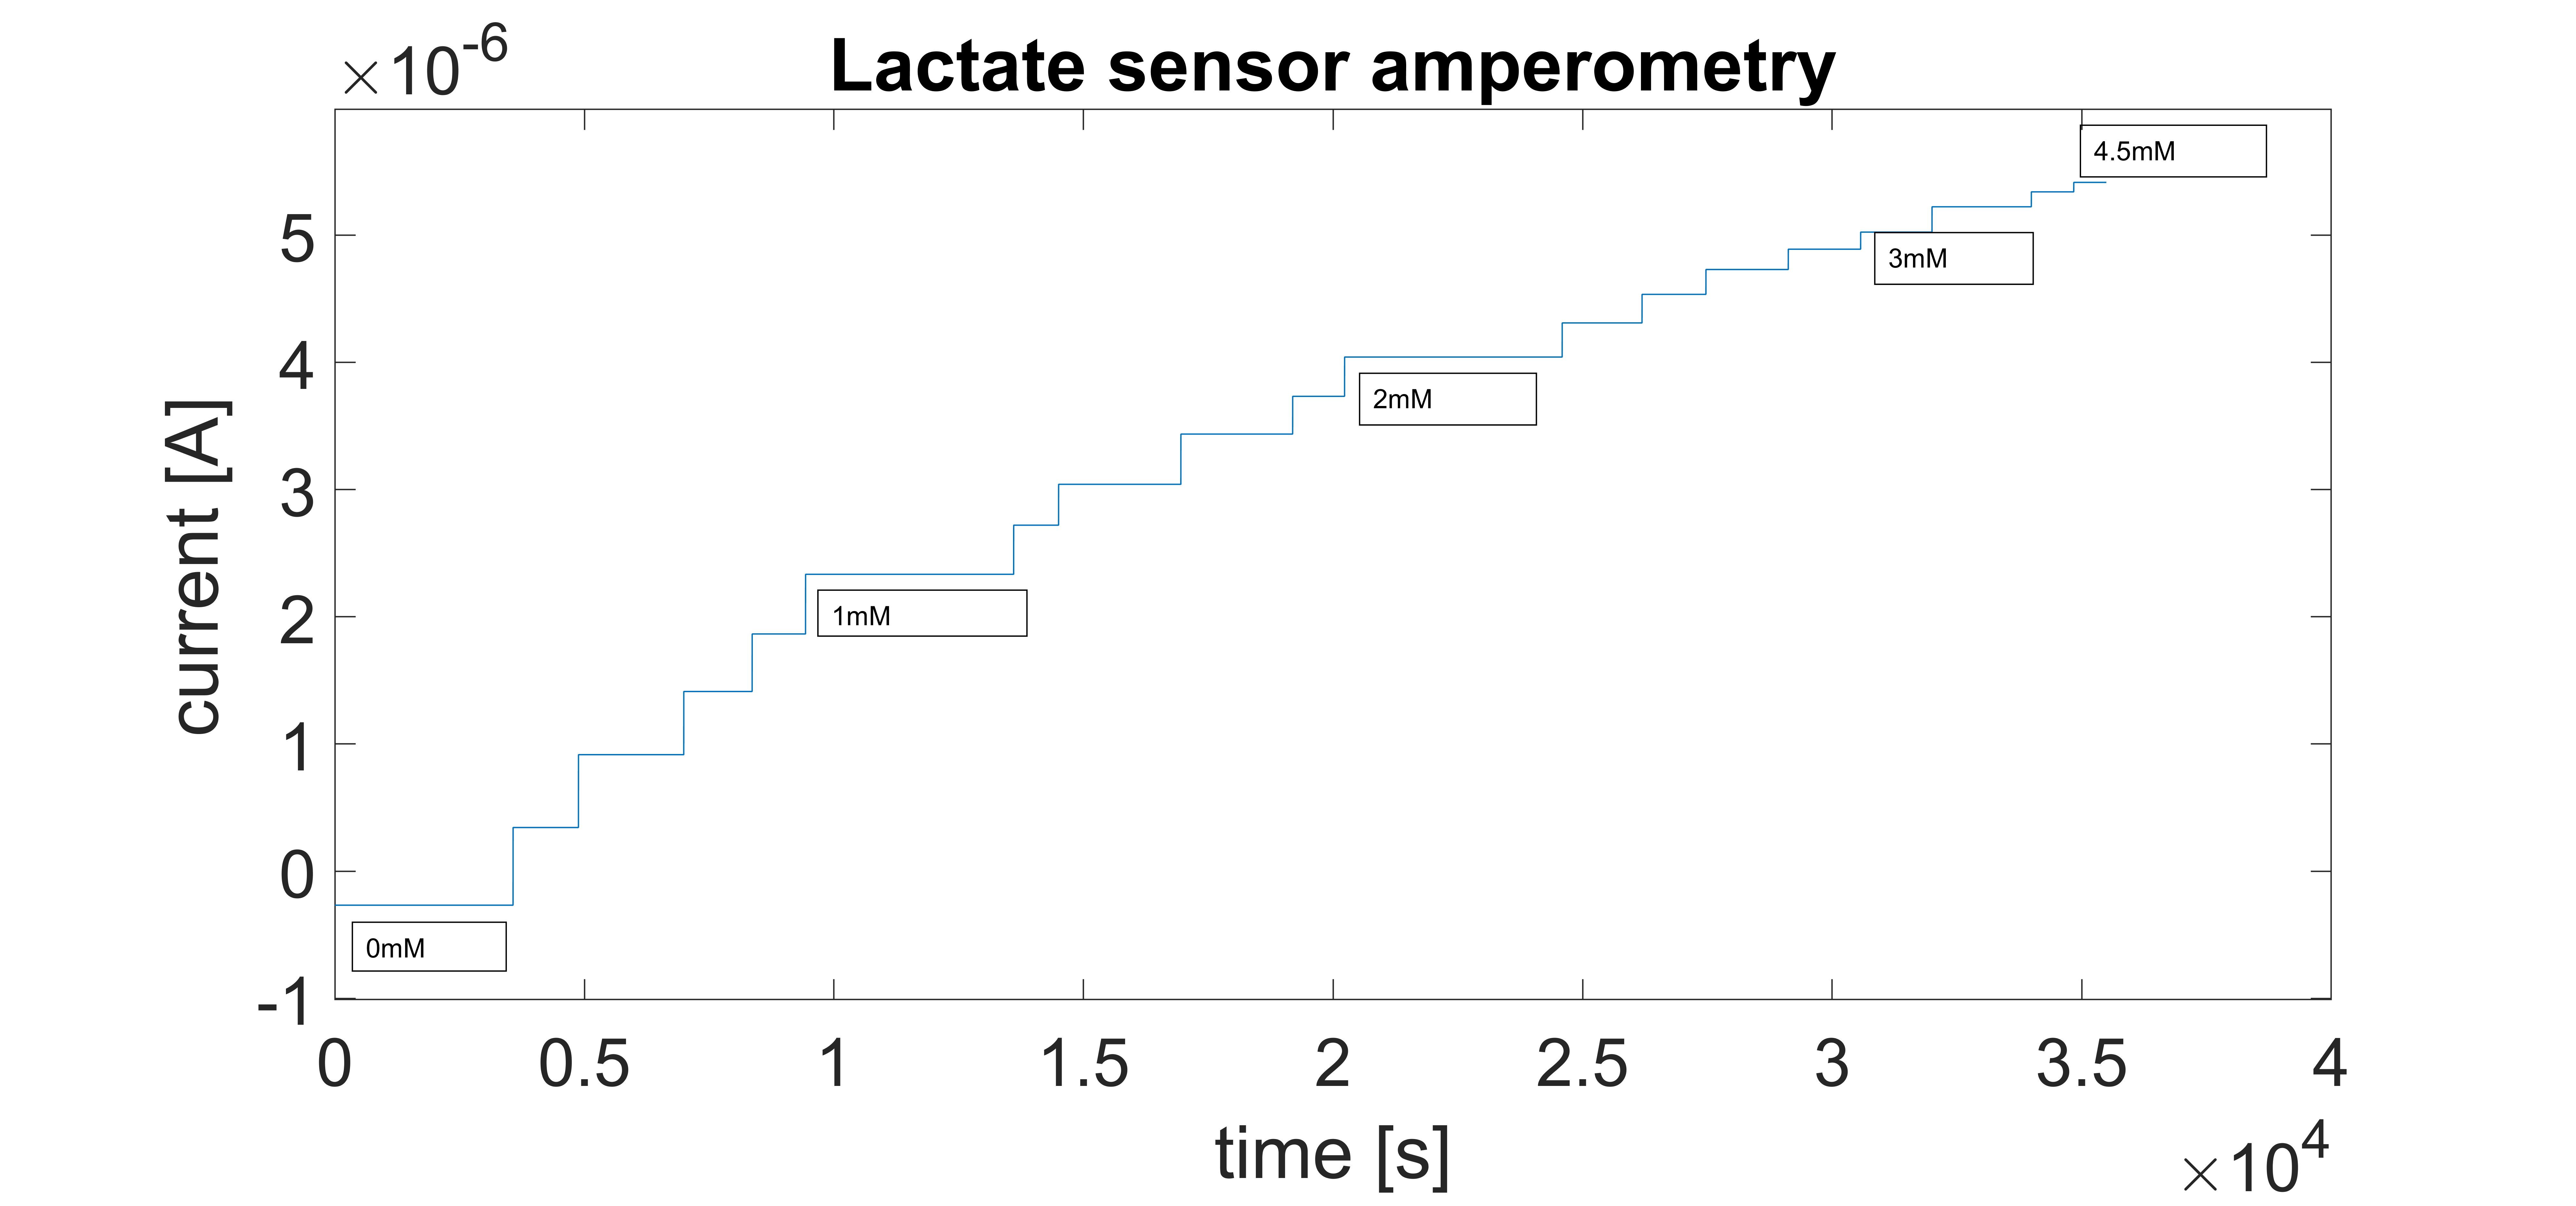
\includegraphics[width=0.5\textwidth]{img/Lactate_fig_1.png}
    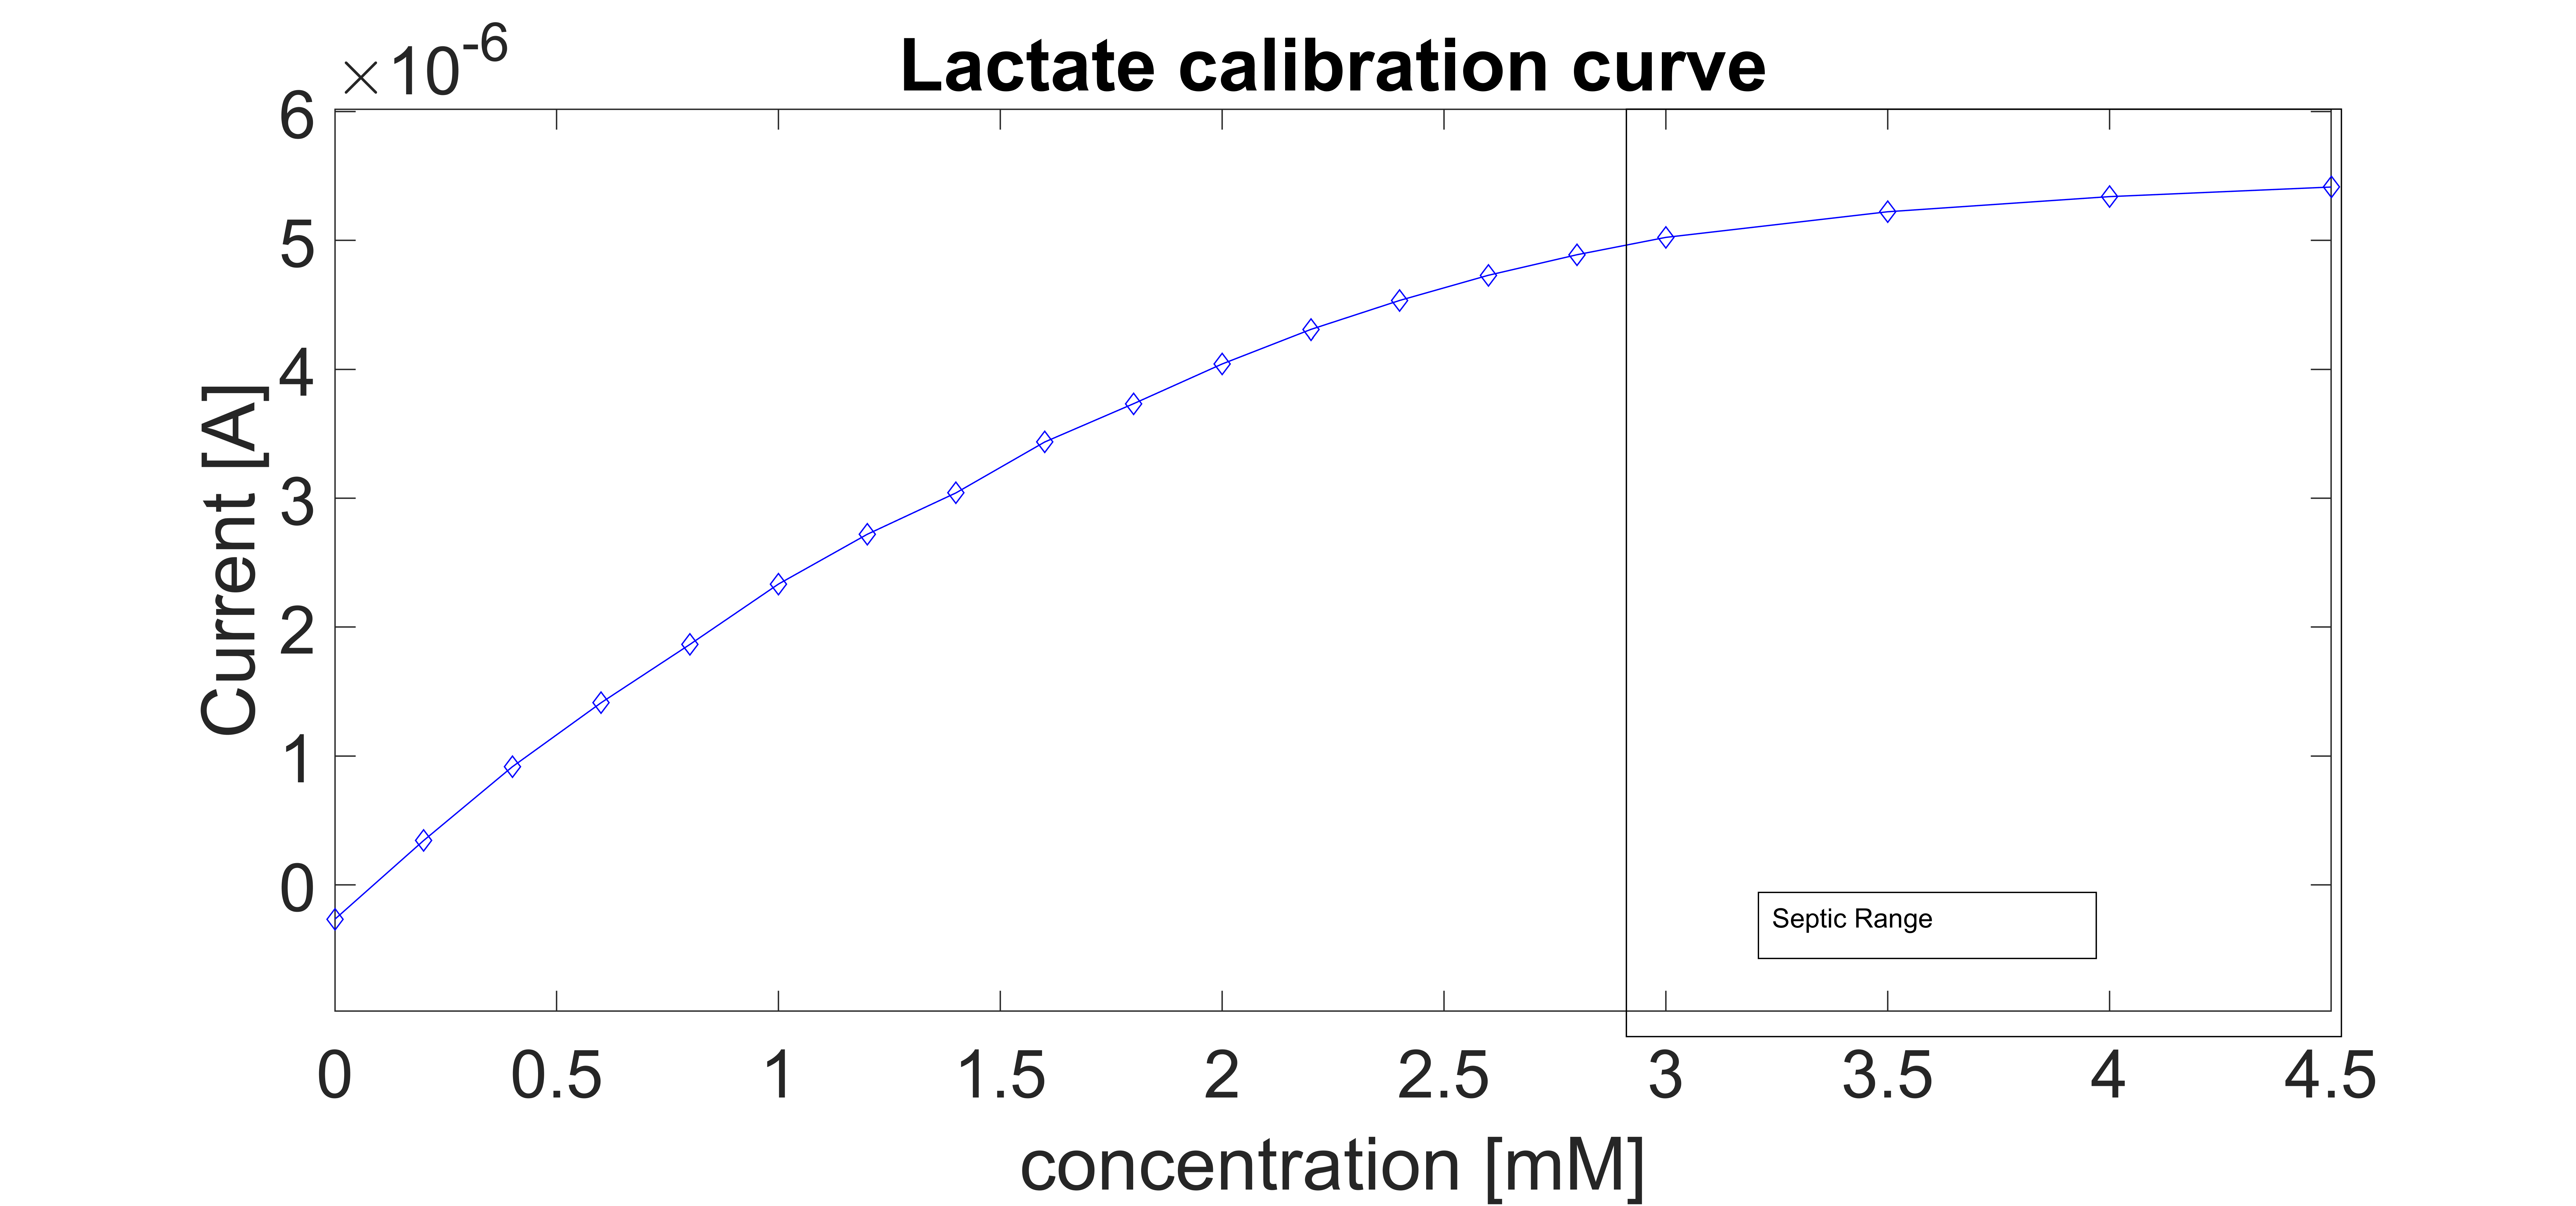
\includegraphics[width=0.5\textwidth]{img/Lactate_fig_2.png}
    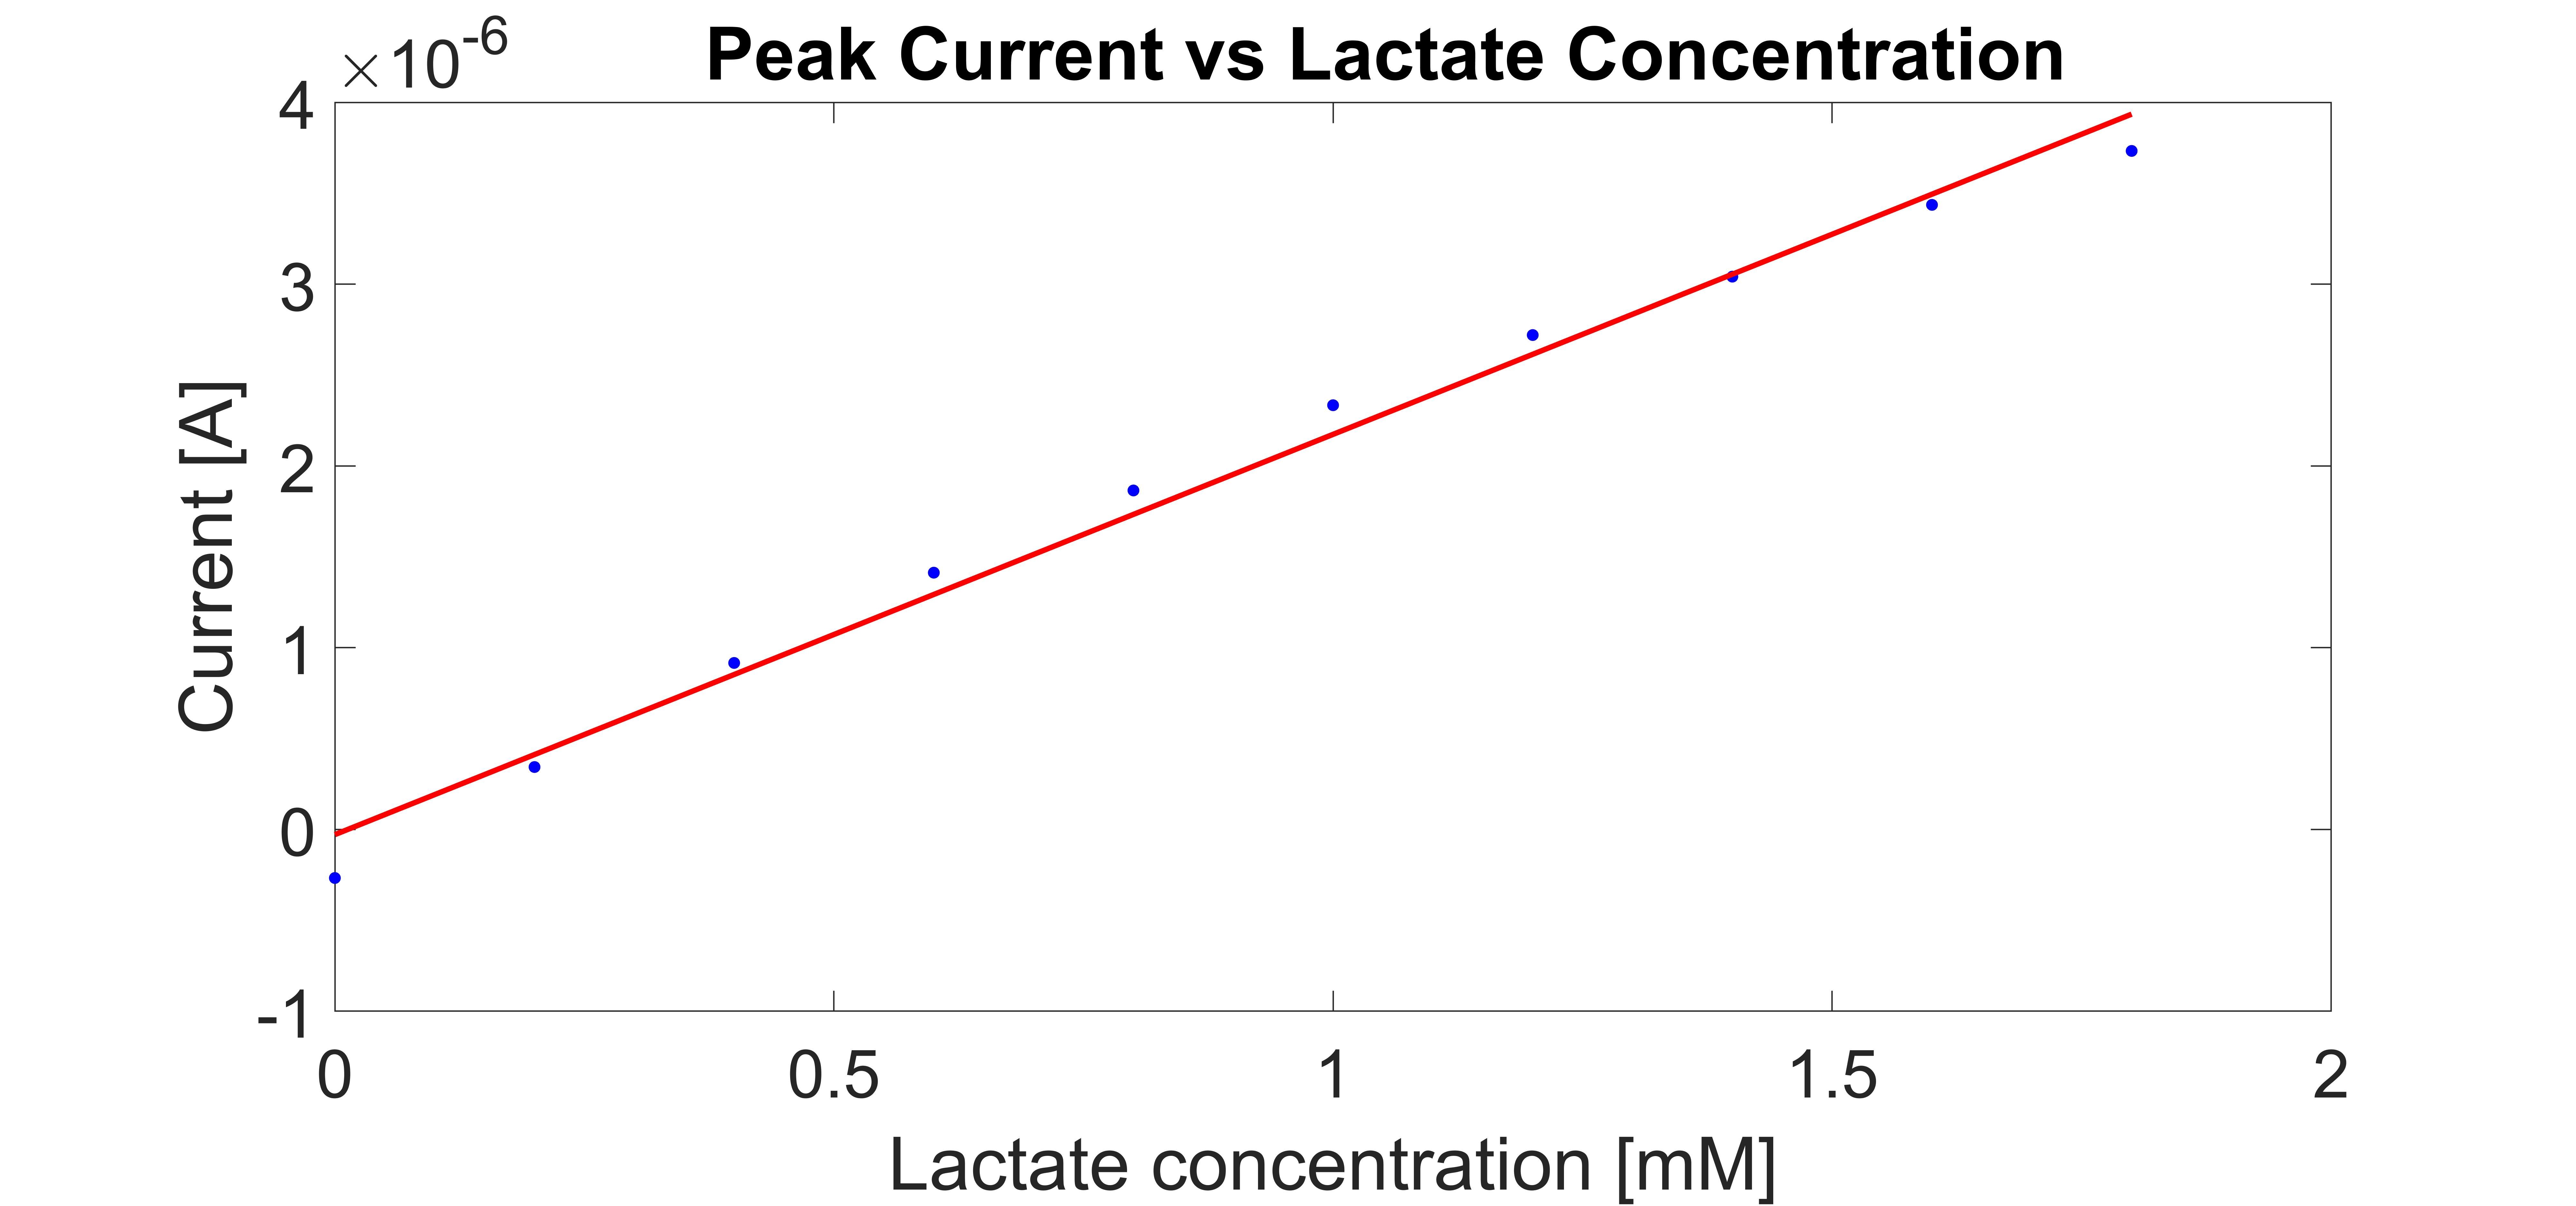
\includegraphics[width=0.5\textwidth]{img/Lactate_fig_3.png}
    \caption{(From top to bottom)(a)Amperometry plot of lactate additions from 0-4.5mM/L lactate solution. (b) Calibration curve of current vs concentration. (c) Linear approximation for the calibration data up to 2mM/L}
    \label{fig:lactate_result}
\end{figure}
In \autoref{fig:lactate_result}(a), the change in current can be observed after each addition of lactate. An average current for each step interval was taken and plotted against time. The time intervals indicate how long the readings took to stabilise, this is of no importance in our conclusions, rather this was due to movement of apparatus or noise. In \autoref{fig:lactate_result}(b) the average currents were then plotted against the lactate concentration  to produce calibration curves as seen in \autoref{fig:lactate_result}(b). Up to a concentration of 2mM/L, the current rises linearly with concentrations shown in \autoref{fig:lactate_result}(c). By plotting the line of best fit, it can be estimated that current increases by 5.48mA for every 1mM additions. \\\\ 
Beyond 2mM/L we still see an increase in current but it is no longer linear and the increase is more shallow at an average increase of  1.20mA per mM of lactate added, a definite plateau indicating poor detection capability in this range. 
\subsection{Multiexponential Rate Extraction on Simulated data}
\vspace{-1cm}
Due to the absence of aptamer data, we test our numerical inverse Laplace multiexponential decomposition using simulated data with superimposed noise. In Plaxco's chronoamperometric study for the detection of Tobramycin, rate constants 100$s^{-1}$ and 500$s^{-1}$ were obtained with no target and saturating target concentration \cite{arroyo2018subsecond}. We have simulated a noise of 10dB, such that it emulates the noise in our instrumentation. In all our simulations, we test with equal values of coefficients [A] and [AT].\\\\
There are three tunable parameters in the algorithm to optimise the solution for the inverse laplace spectra $\mathbf{G}(k)$. 1) The solution space for $\mathbf{G}(k)$. 2) Resolution of points in the solution space. 3) The value of $\alpha$, the regularizer. \\\\
We constrain the solution space between $k = 10s^{-1}$ and $k = 800s^{-1}$). We ran a parameter analysis using alpha to determine an optimum value that provided the most accurate solution (\autoref{alpha}). At smaller values of $\alpha$ ($\alpha = 0.1$), the output waveform is spiky. At larger values of $\alpha$, the inverse laplace is excessively smoothed, where the peaks are widened. we therefore chose the $\alpha = 1$, due to the smooth output waverform, without widening the peaks of $\mathbf{G}(k)$. We therefore use $\alpha = 1$ in future simulations with the inverse laplace method, as it produces the most accurate and representative results, out of all the values of alpha tested.\\\\
Testing the algorithm on simulated double exponential data (with rates $k_{A}$ = 100$s^{-1}$ and $k_{AT}$ = 500$s^{-1}$) with the presence of noise, we can observe two distinct peaks centred at the two relevant rate constants of the signal (Figure \ref{multiexp}). In order for the algorithm to test the rate constants for the target bound and target unbound aptamer, we need to assess the ability of the algorithm to resolve rate constants that could potentially be closer. We find that the resolution is accurate for $k_{A}$ = 150$s^{-1}$ and $k_{AT}$ = 450$s^{-1}$ (\autoref{multiexp_2}), but as the two rate constants are brought closer together, the peaks overlap, forming a bimodal distribution (Fig. \ref{multiexp_3}). At ($k_{A}$ = 250$s^{-1}$ and $k_{AT}$ = 350$s^{-1}$ (\autoref{multiexp_4})), only a single peak is observed. The ability for this numerical inverse Laplace method to resolve rates that are close together is affected by the presence of noise in the raw signal, and the resolution of $\mathbf{G}(k)$ defined. More realistic experimental data would help characterise the nature of the noise and resolution of the $\mathbf{G}(k)$ is limited by computational time.\\\\
%\belowdisplayskip=0pt\relax
%\begin{equation}
%     f'(t) = awgn(f(t),SNR = 10dB)
%\end{equation}
To obtain the coefficients of the each exponential decay, we can use the normalised intensity values that is output from the numerical inverse Laplace (\autoref{multiexp}), or take the central value of the two peaks for the rate constant, and use the numerical inverse laplace algorithm to extract the coefficients.
\begin{figure}[H]
    \centering
    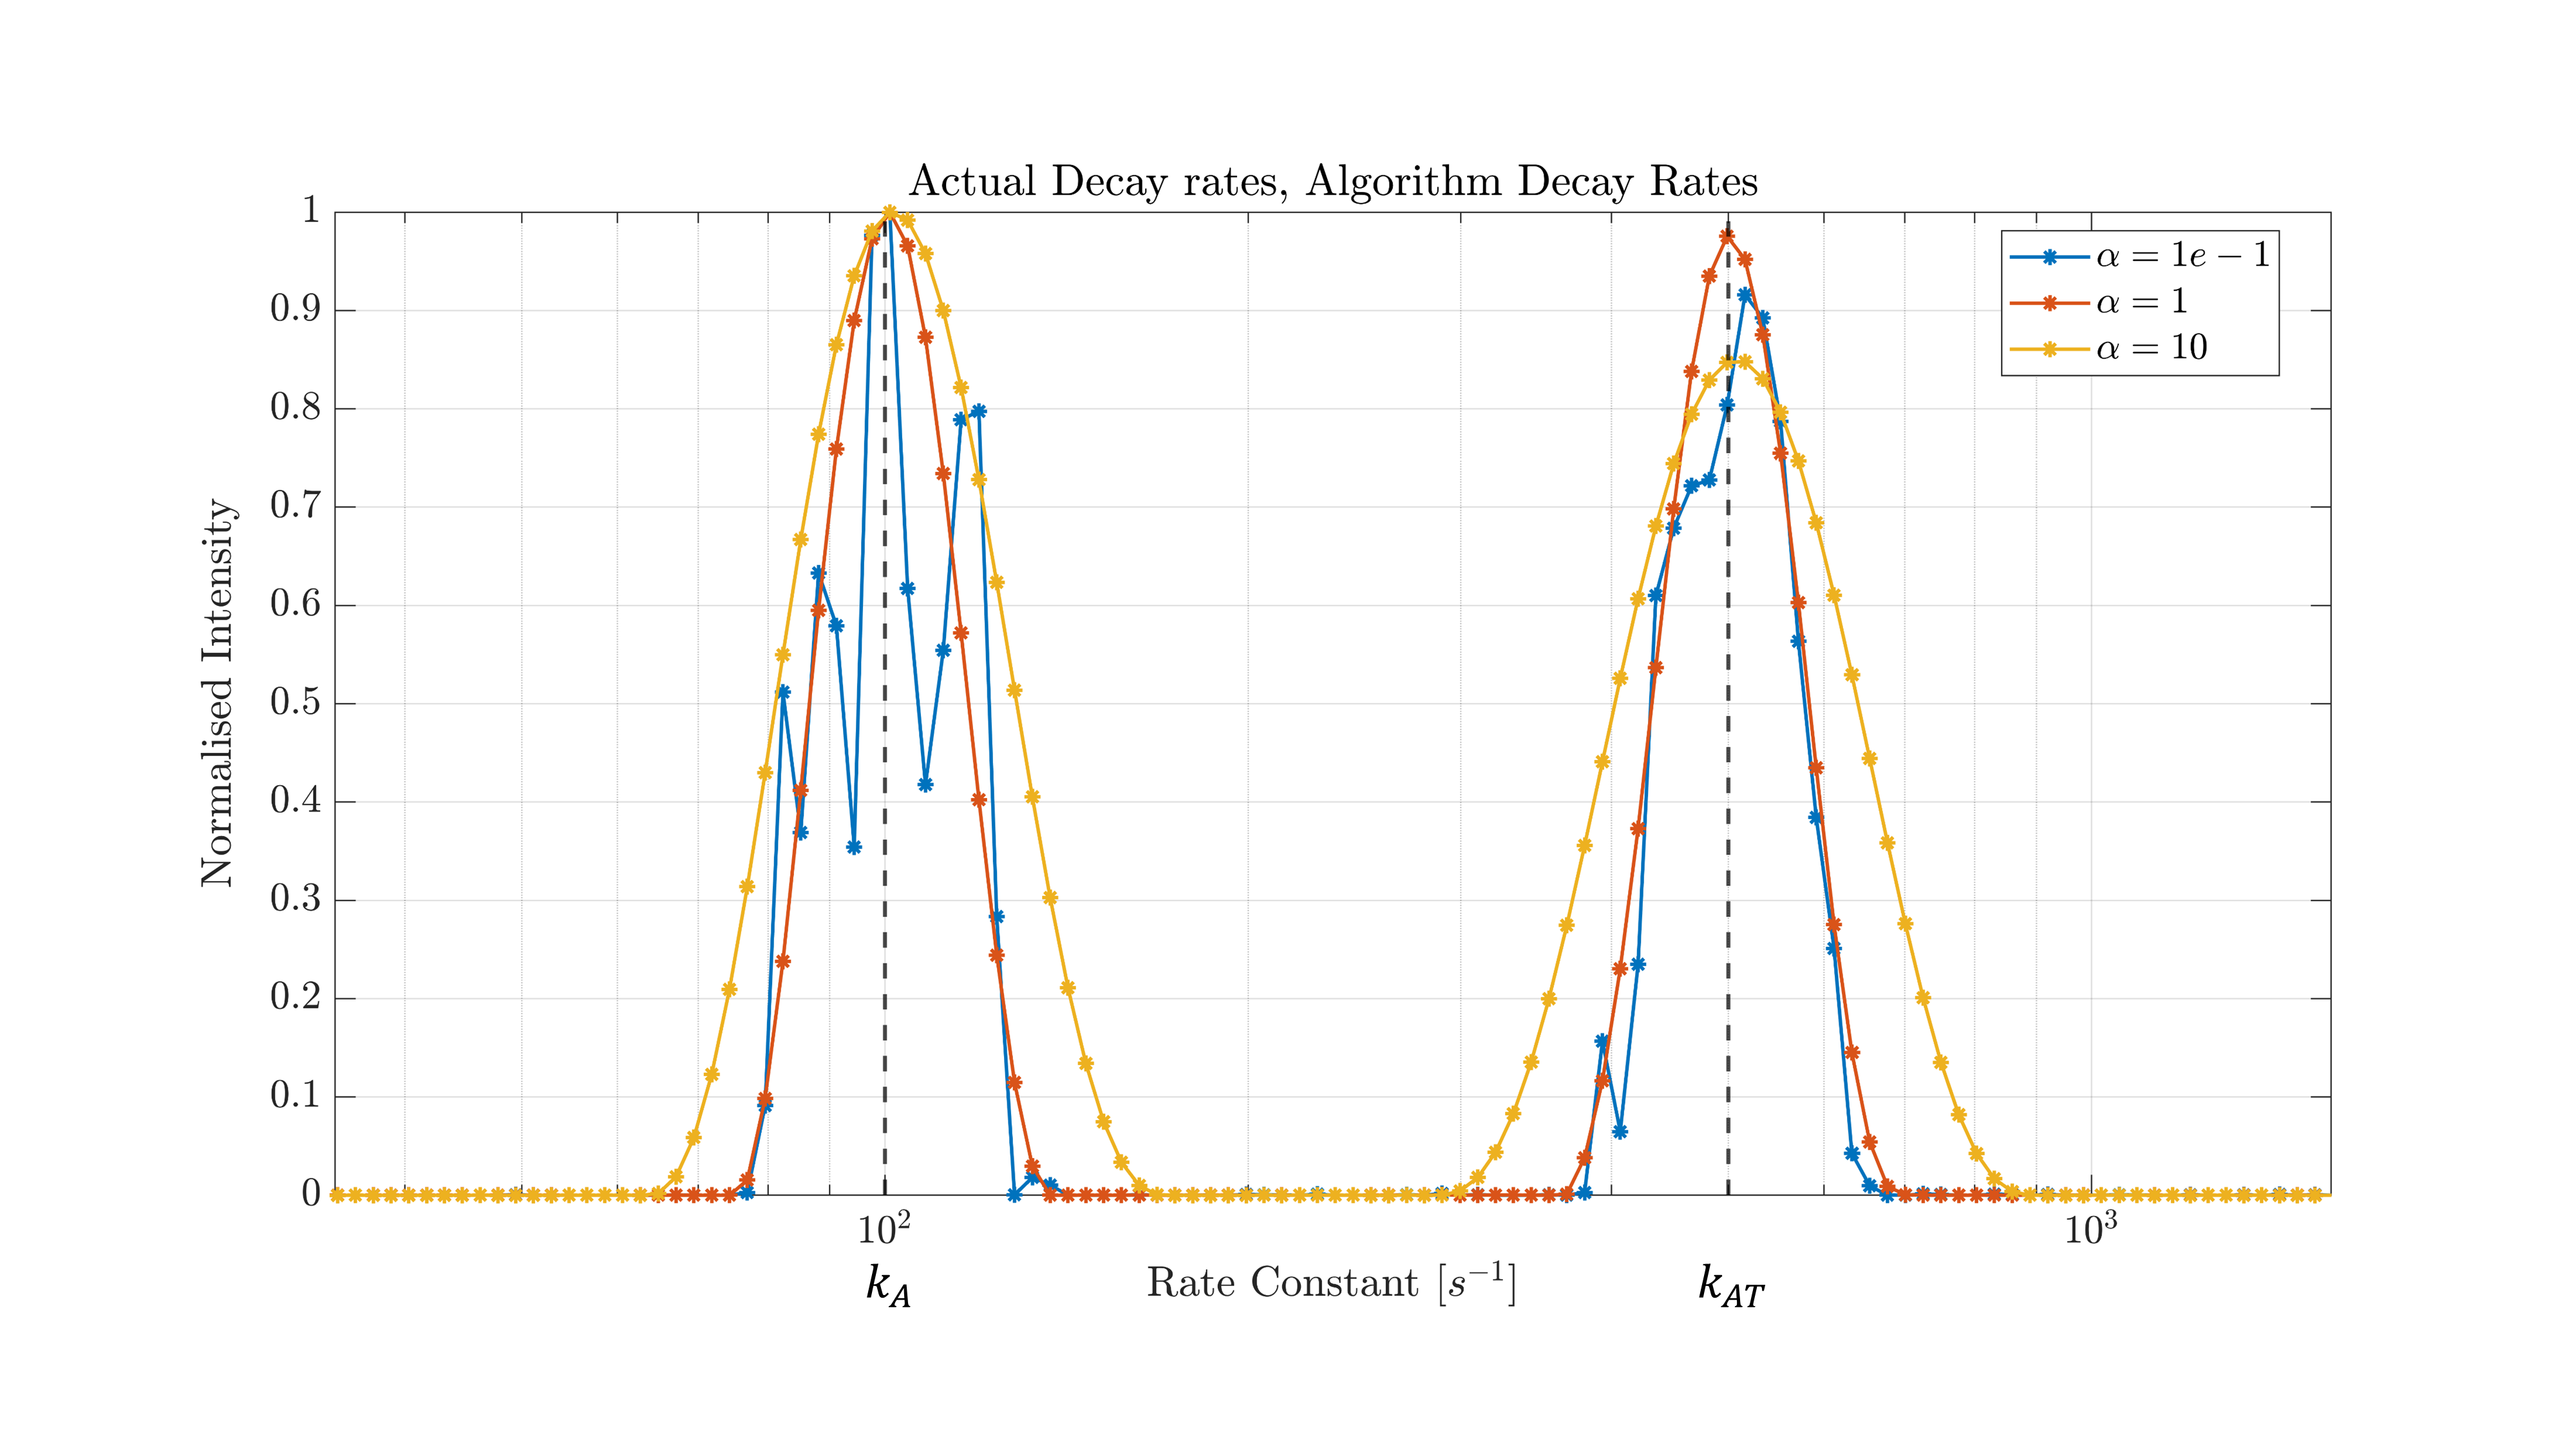
\includegraphics[width = 0.5\textwidth]{img/alpha_testing_annotate.png}
    \caption{Parameter sensitivity analysis using three values of $\alpha$. $\alpha = 1$ provided the best solution that represented the intrinsic rate constants present in the raw signal.}
    \label{alpha}
\end{figure}
\begin{figure}[H]
    \centering
    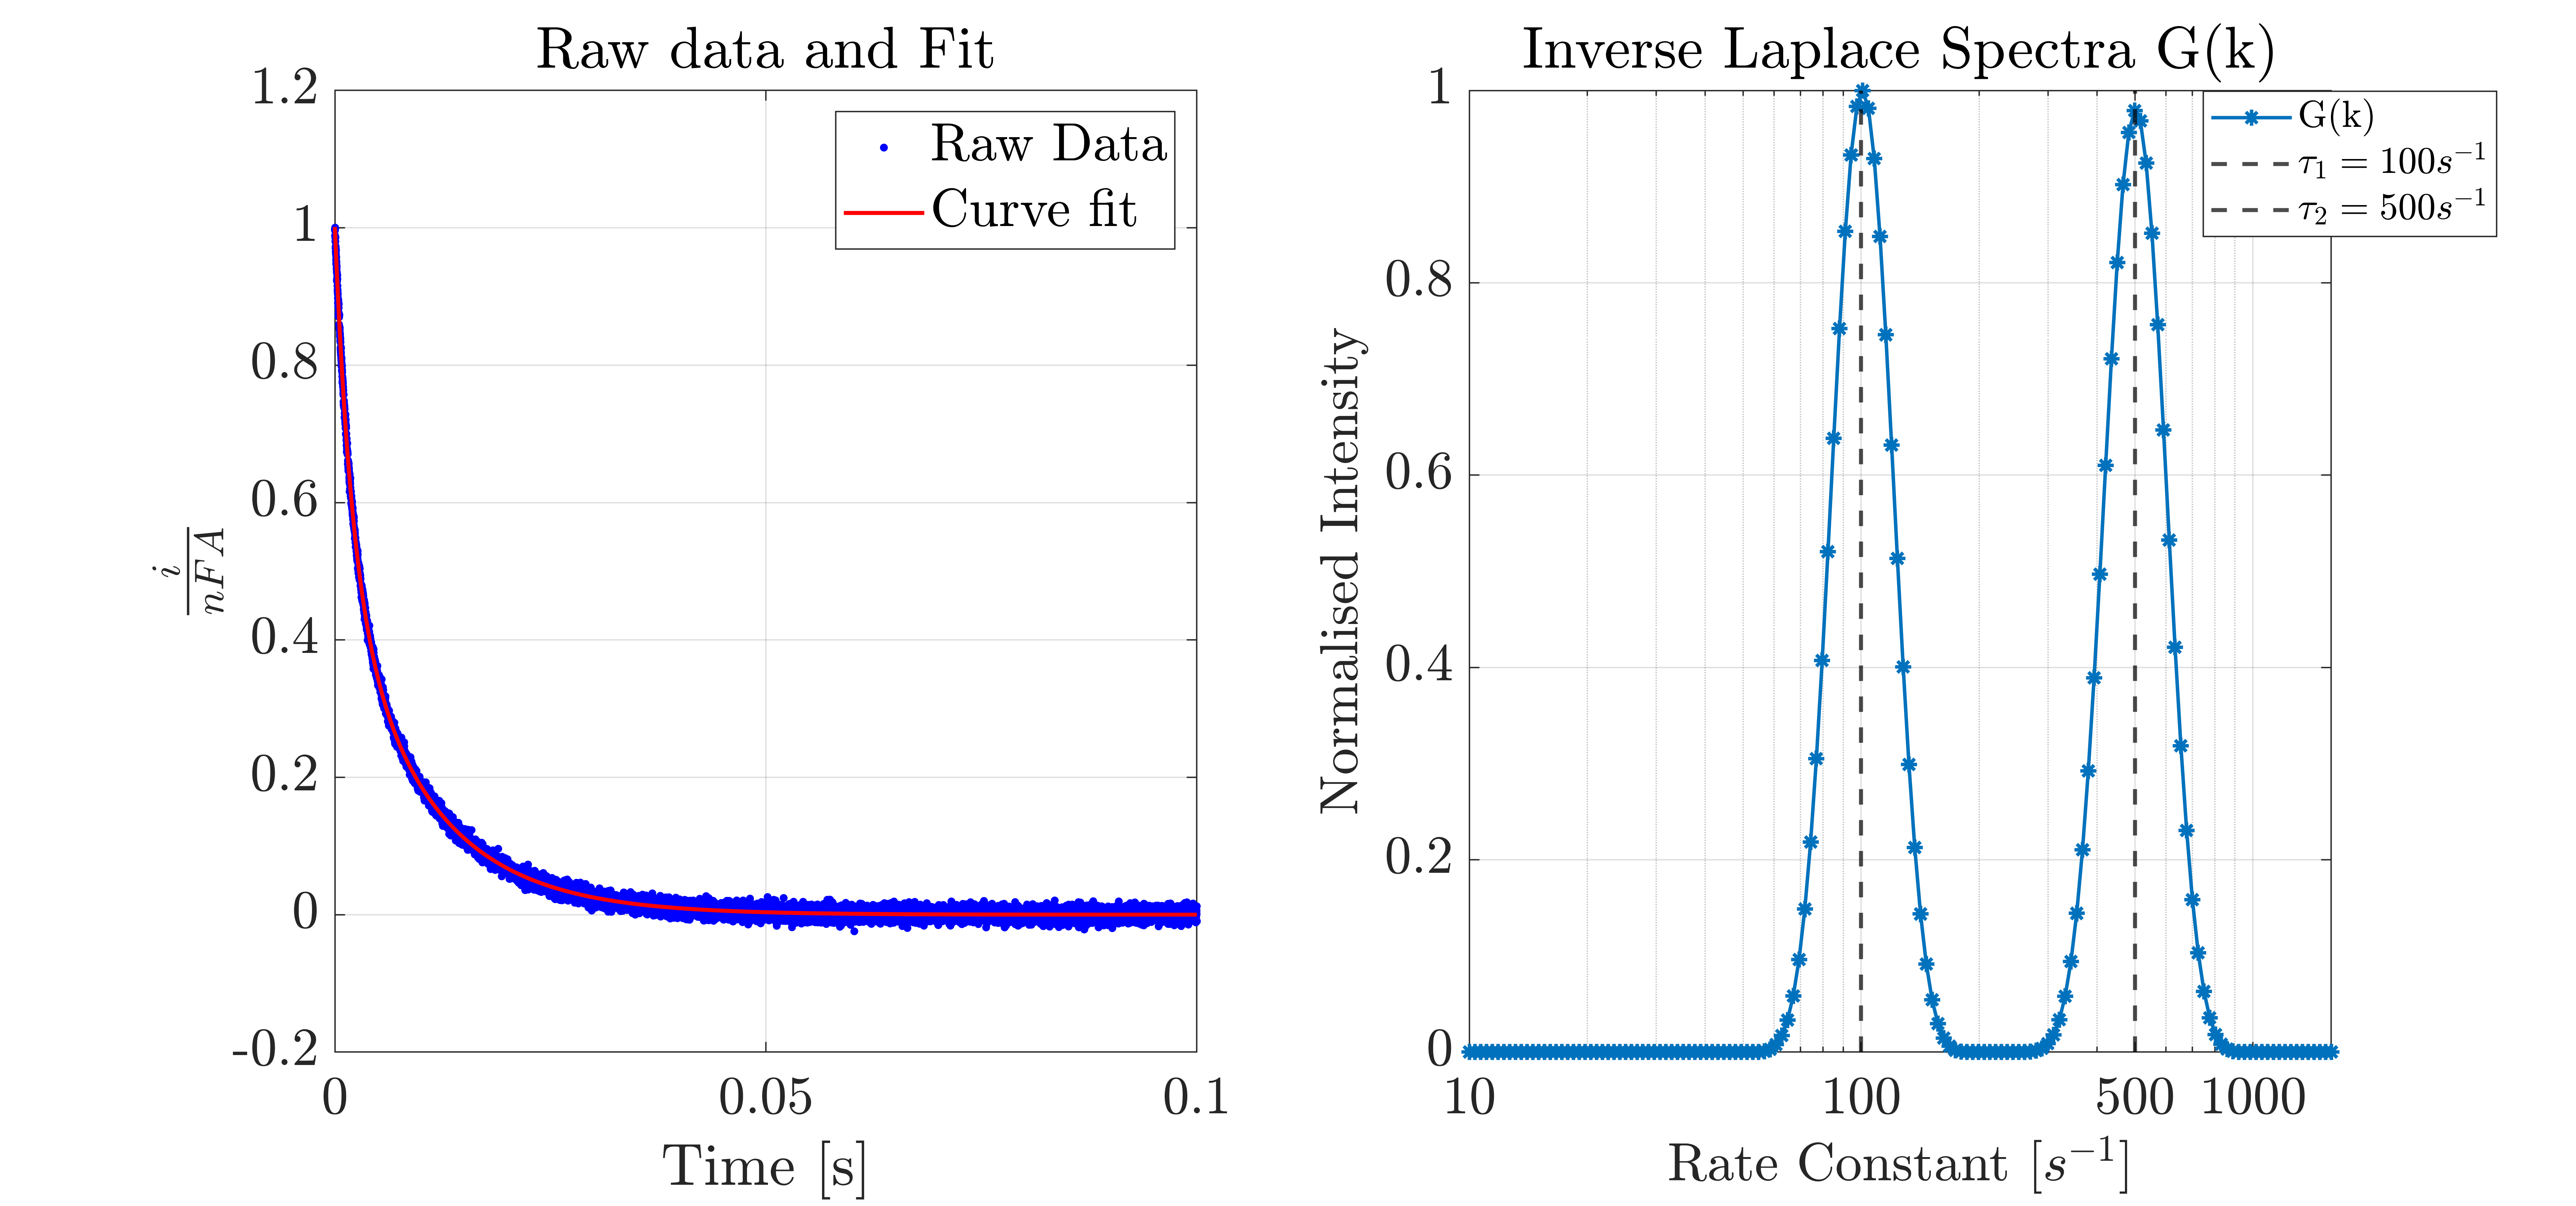
\includegraphics[width = 0.5\textwidth]{img/Inv_Laplace_results.png}
    \caption{Inverse Laplace Algorithm performance against simulated data with rate constants $k_{A} = 100s^{-1}$ and $k_{AT} = 500s^{-1}$}
    \label{multiexp}
\end{figure}
\begin{figure}[H]
    \centering
    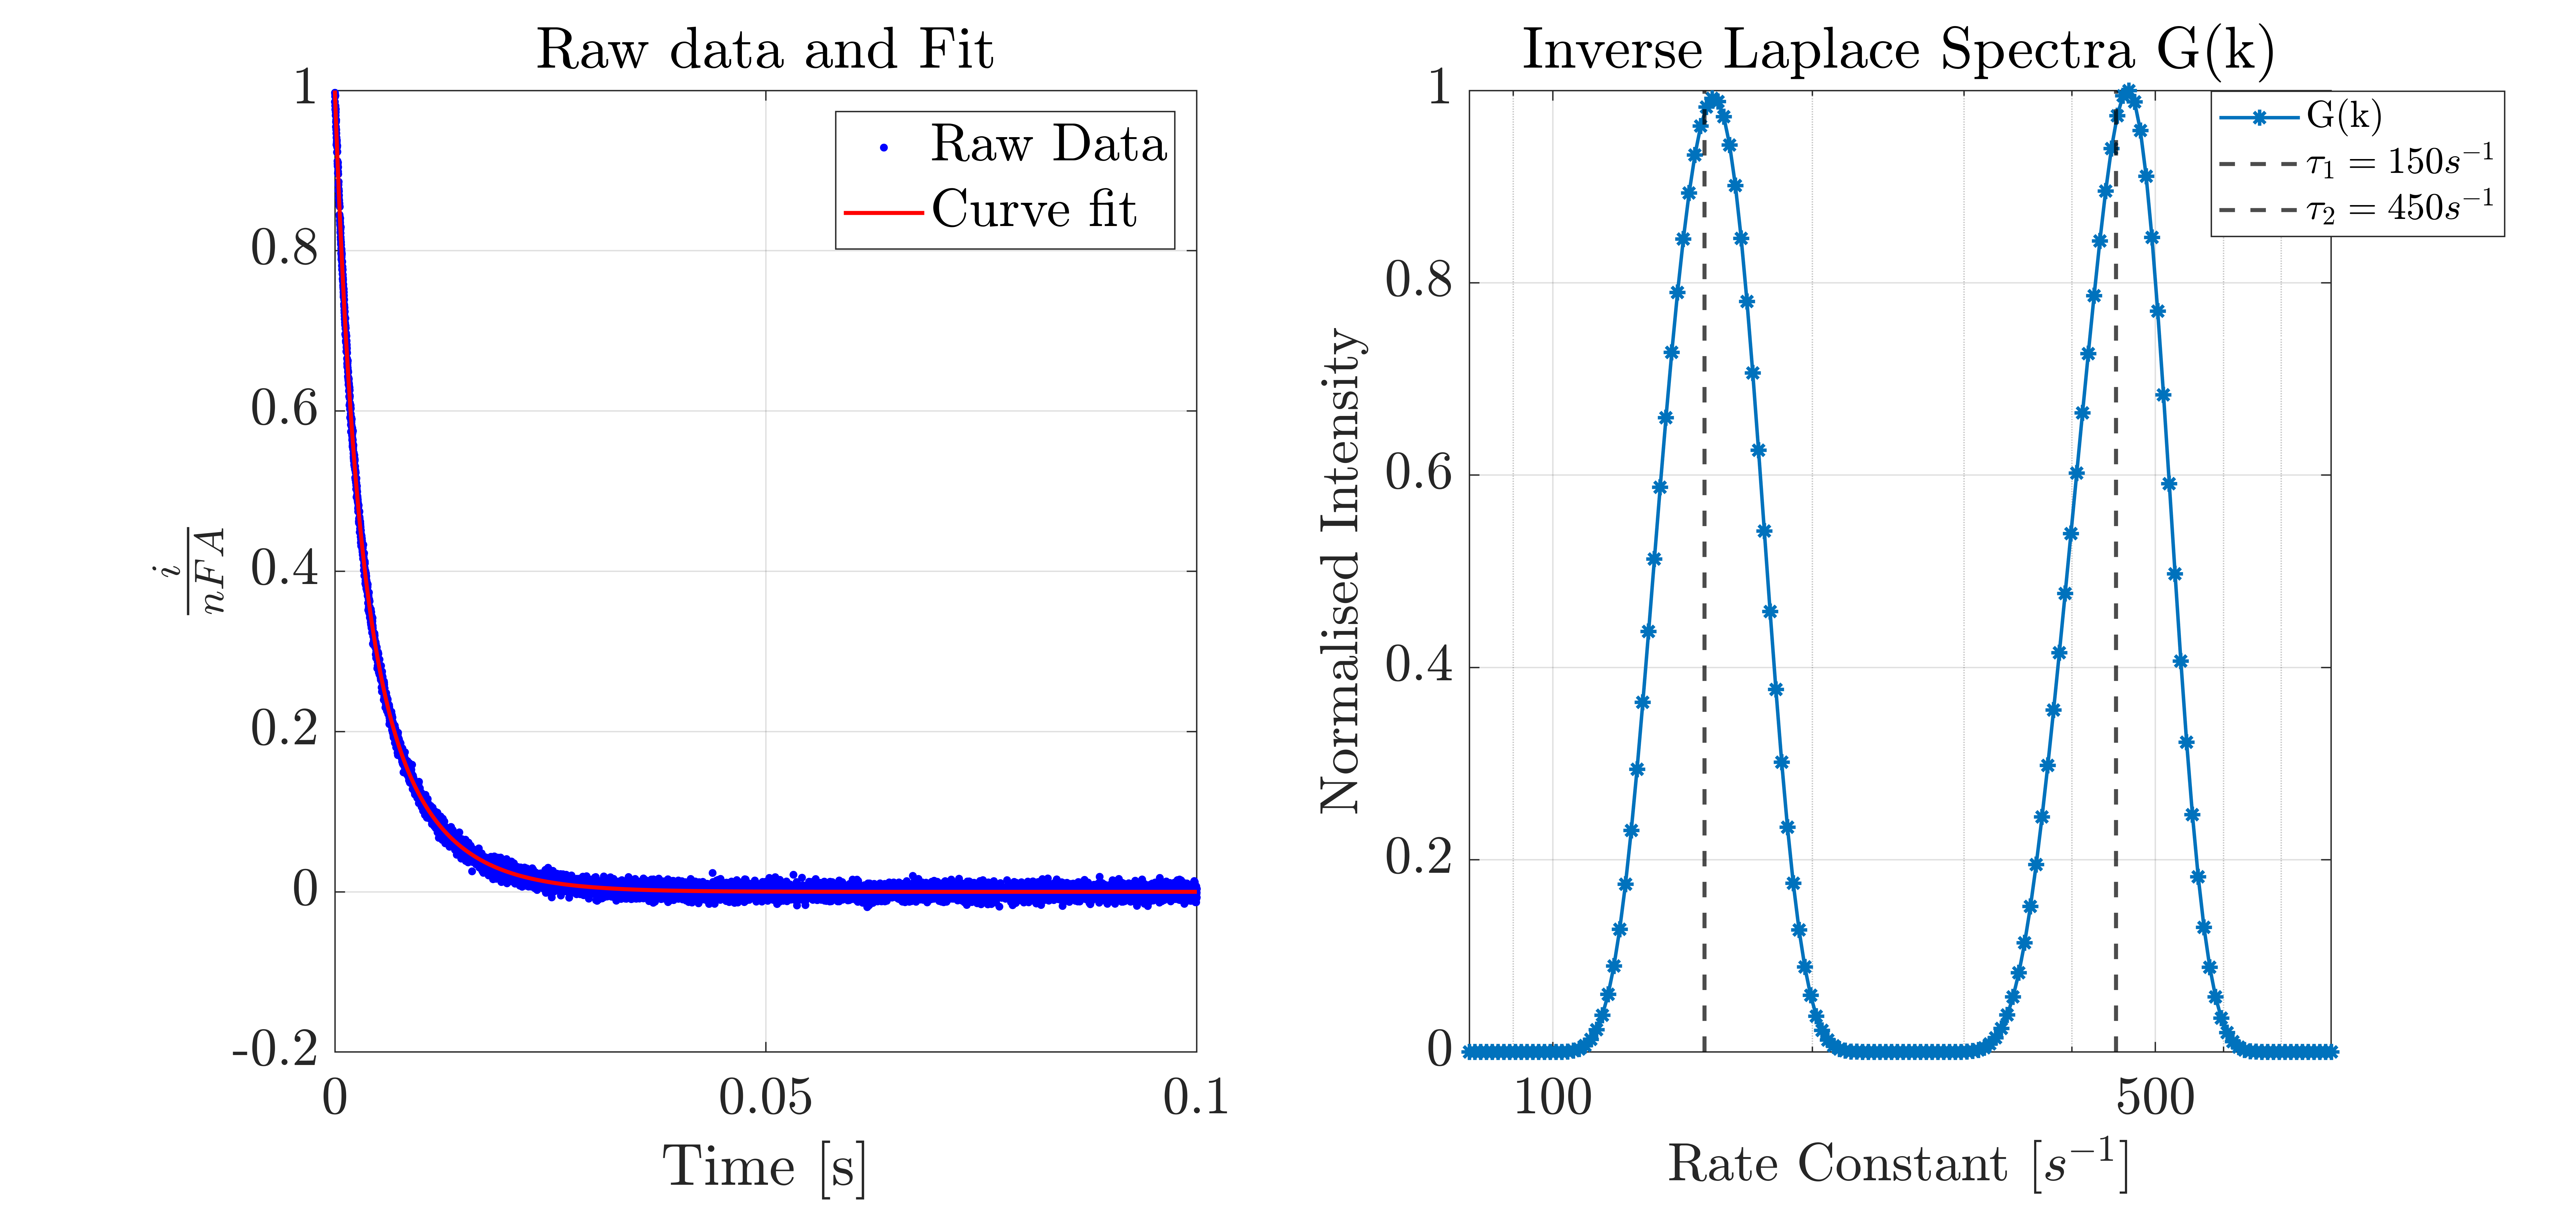
\includegraphics[width = 0.5\textwidth]{img/Inv_laplace_150_450.png}
    \caption{Inverse Laplace Algorithm performance against simulated data with rate constants $k_{A} = 150s^{-1}$ and $k_{AT} = 450s^{-1}$}
    \label{multiexp_2}
\end{figure}
\begin{figure}[H]
    \centering
    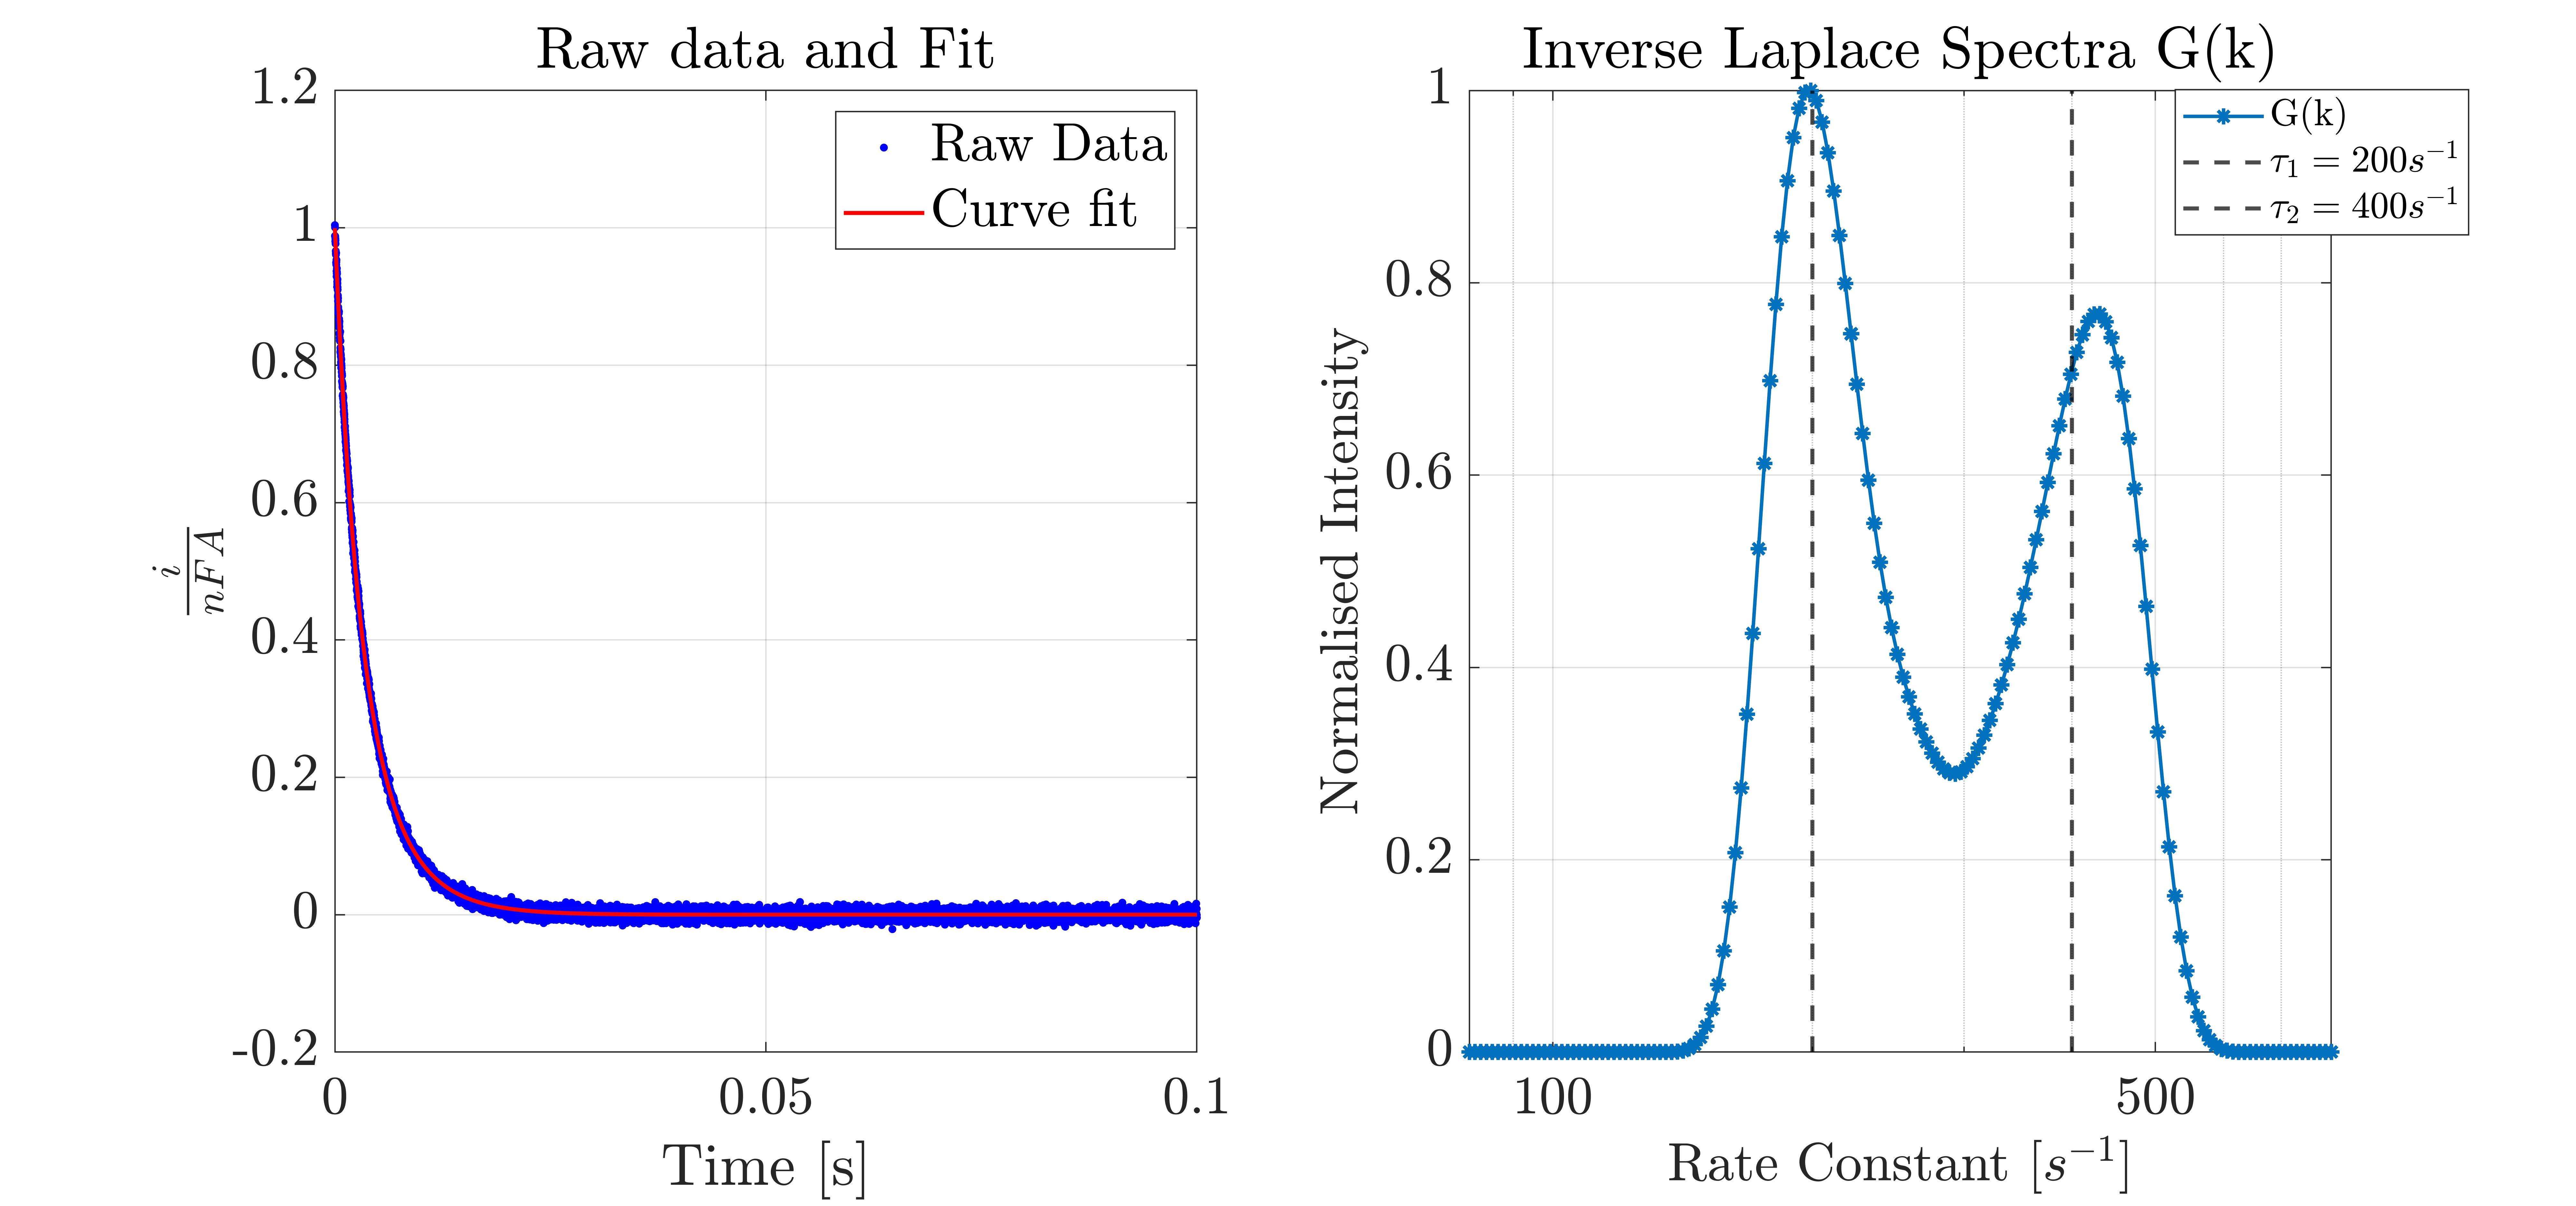
\includegraphics[width = 0.5\textwidth]{img/Inv_laplace_200_400.png}
    \caption{Inverse Laplace Algorithm performance against simulated data with rate constants $k_{A} = 200s^{-1}$ and $k_{AT} = 400s^{-1}$. Overlap in peaks, however can still distinguish the two peaks as distribution is bimodal.}
    \label{multiexp_3}
\end{figure}
\begin{figure}[H]
    \centering
    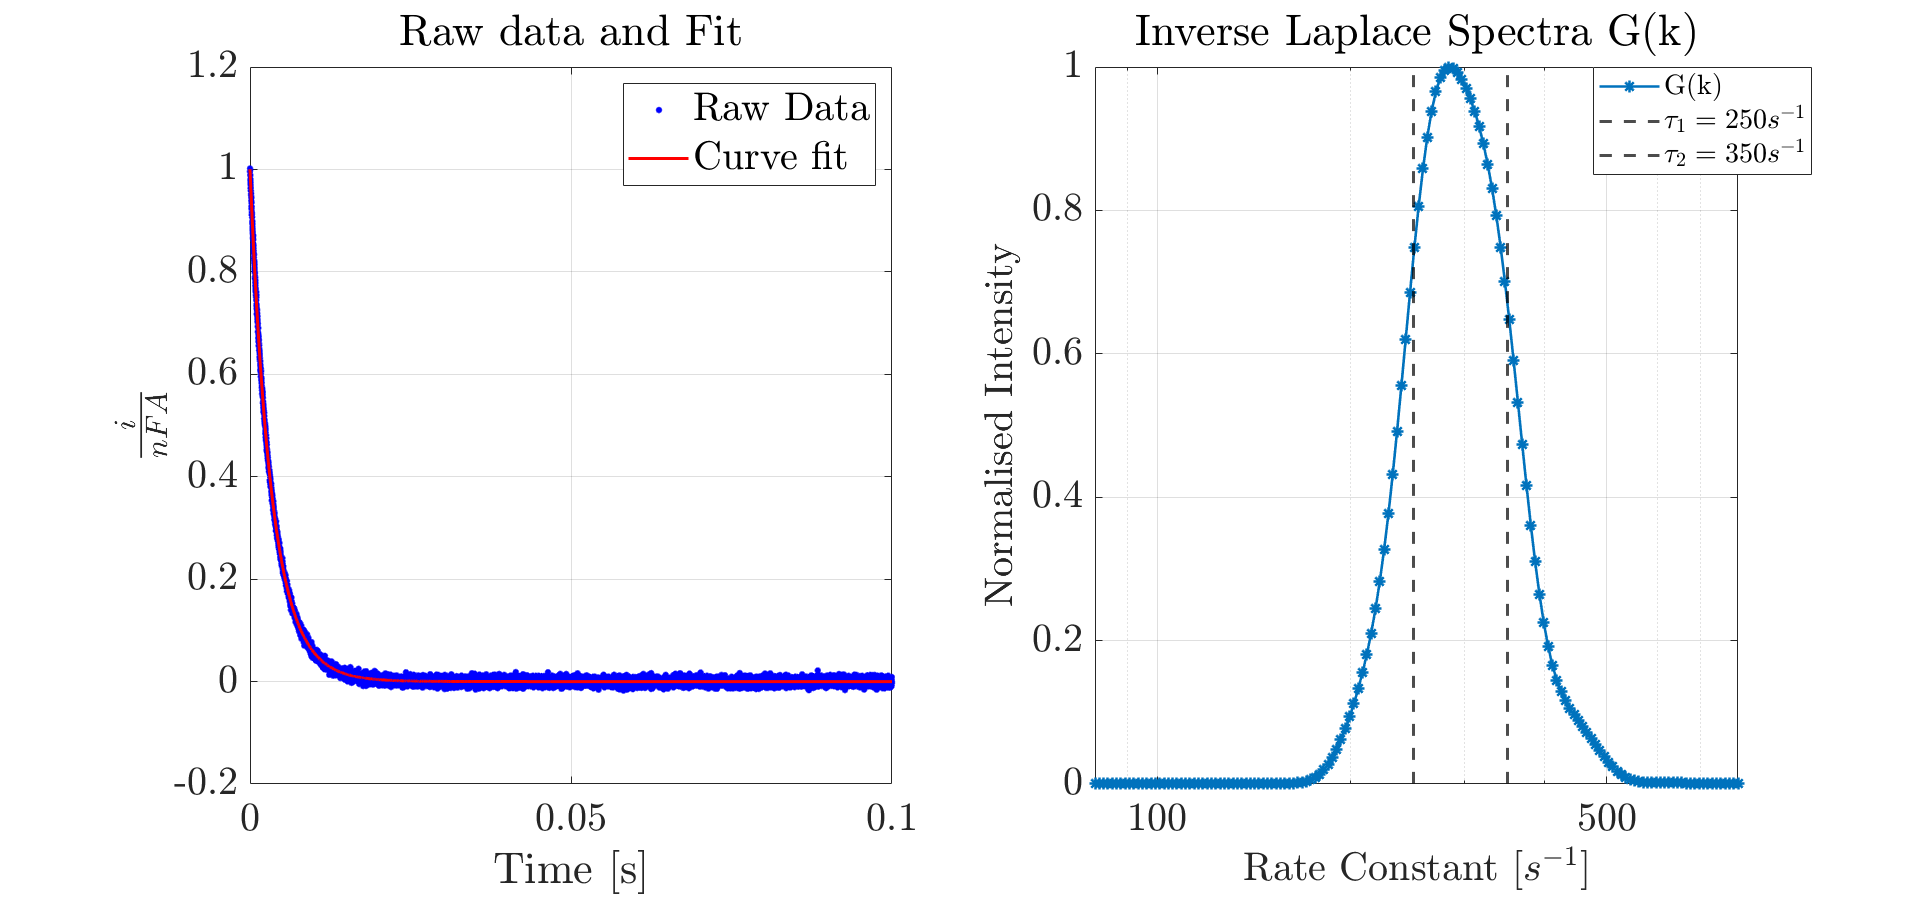
\includegraphics[width = 0.5\textwidth]{img/Inv_laplace_250_350.png}
    \caption{Inverse Laplace Algorithm performance against simulated data with rate constants $k_{A} = 250s^{-1}$ and $k_{AT} = 350s^{-1}$. The rate constants are close such that the two peaks have merged into one peak.}
    \label{multiexp_4}
\end{figure}
\subsection{Coarse-grained Aptamer Model Predictions}
Assuming electron transfer is effectively instantaneous at small distances in a Nernstian process through the SAM \cite{finklea1992electron,smalley1995kinetics}, we can use the collision model \cite{huang2013random} to estimate the probability for an electron transfer event from occurring for a given aptamer length. The length of a Methylene-Blue molecule is 14.47$\angstrom$ \cite{dotto2015adsorption}. This is equivalent to a distance of 1.45nm. Using this distance as the threshold value, we obtain the following probabilities that a collision occurs for the various aptamer lengths tested (\autoref{dep_plot_2}):
\begin{figure}[H]
    \centering
    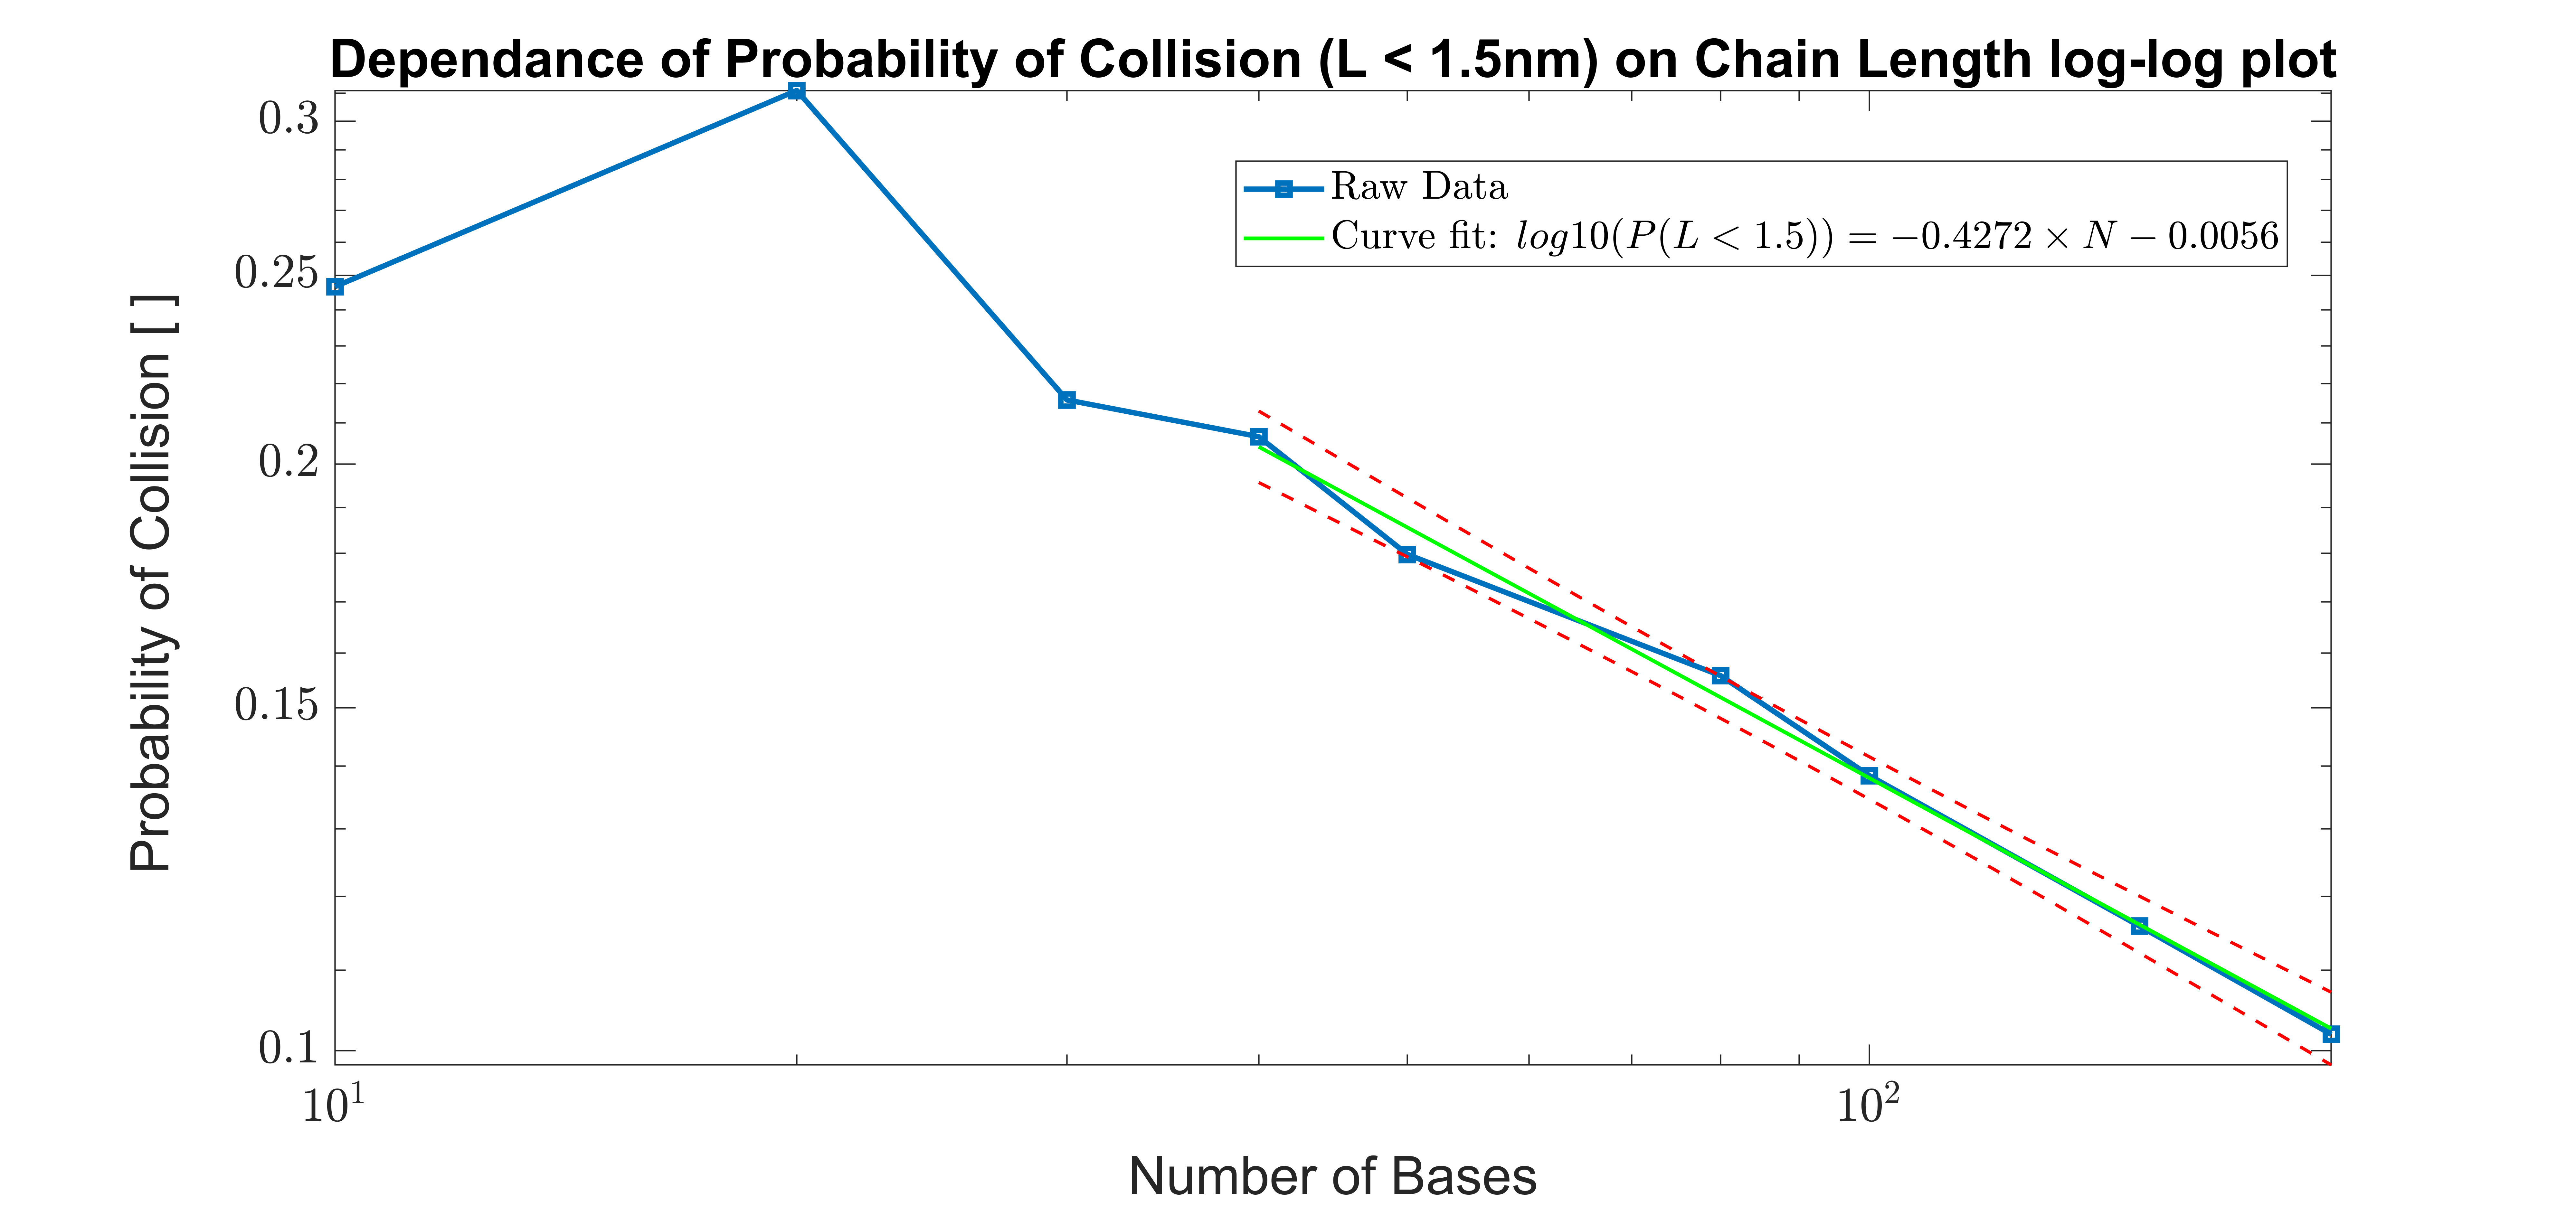
\includegraphics[width = 0.5\textwidth]{img/Length_dep_bases_log.png}
    \caption{Dependance of probability of collision (L $<$ 1.5nm) on the base length for the freely-jointed chain model of the aptamer. Log-log plot. Curve fit shows a -0.4272 dependence of log10(P$<$1.5nm) to log10(N) where N is the number of bases.}
    \label{dep_plot_2}
\end{figure}
\noindent{We can see that by plotting the length in a log scale, the collision probability has a linear dependence on the base length. These estimates are comparable to studies done by Plaxco et al. (\autoref{plaxco_plot} \cite{arroyo2018subsecond}) who found apparent electron transfer rate exhibits a power-law dependence on chain length, N (number of monomers)
with an exponent of 1.166 $\pm$ 0.09.}
\begin{figure}[H]
    \centering
    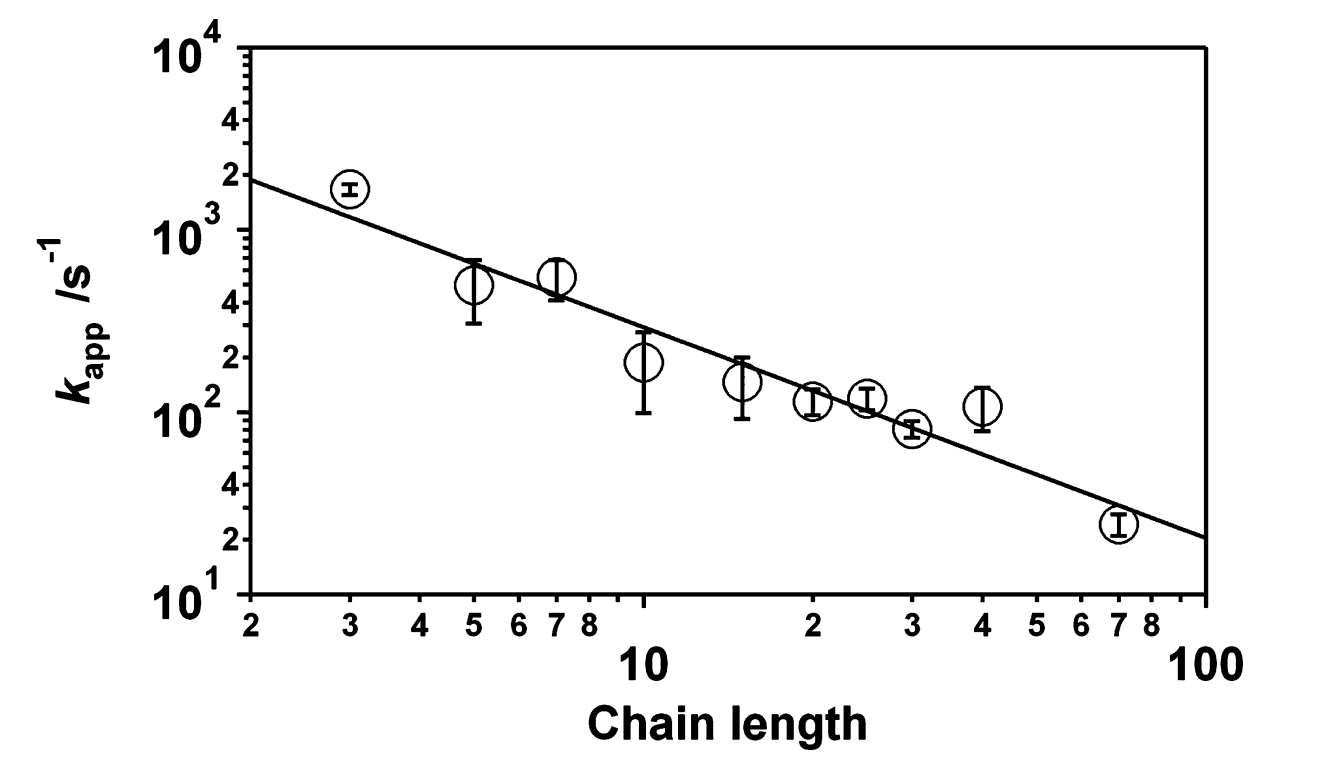
\includegraphics[width = 0.5\textwidth]{img/Plaxco_k_app_vs_length.png}
    \caption{Dependence of rate constant on the base length for the freely-jointed chain model of the aptamer. Log-log plot. The apparent electron transfer rate exhibits a power-law dependence on chain length, N (number of monomers) with an exponent of 1.166 $\pm$ 0.09. \cite{uzawa2010mechanistic}}
    \label{plaxco_plot}
\end{figure}


\newpage
\section{Discussion}

\subsection{Nitrite Investigations}
We have found that use of both disposable and reusable gold electrodes are suitable for measuring nitrite concentrations in solution as mentioned previously in background. (Our chosen nitrite concentrations reflect the normal physiological levels and expected elevation in septic patients.) Therefore, DPV is found to be a reliable method of measuring the electrochemical activity of nitrite in solution. However, using our parameters, each measurement takes 405s. This may prove a challenge for both real-time monitoring and in the clinical setting.\\\\
DPV voltammograms from nitrite experimentation reveals a common peak where the peak current recorded increases with higher concentrations of nitrite, across all experiments, between 0.7 and 0.8 V, which is as expected from literature \cite{article}. Small peaks corresponding to an unknown species was reliably detected at 0.2 V in PBS only experiments, but were not present in albumin experiments. Increased noise and smoothing may have eliminated this peak. We hypothesise that small peaks may have resulted from oxygen impurities in solution.\\\\ 
The albumin experiments showed that at low nitrite concentrations (below 16 µM), the sensitivity is comparable to results without albumin. However, at higher nitrite concentrations, the sensitivity increases to 7nA µM-1, with a marked change in the calibration curve (Figure 8), suggesting interactions between the nitrite and the albumin. Detected current was greater overall in albumin experiments compared to without albumin. This contradicts the hypothesis that albumin adsorbs onto the electrode surface, interfering with the electrode's ability to detect nitrite.

\subsection{Hydrogen Peroxide Investigations}
To perform hydrogen peroxide electrochemical detection using the microneedles platform, we have conducted chronoamperometry, an electrode calibration experiment, with gold electrodes over a range of hydrogen peroxide concentrations. The calibration process was facilitated by the reactions between hydrogen peroxide and Prussian blue PEDOT:PSS-PB complex, as shown in \autoref{eqn:h2o2redox1} and \ref{eqn:h2o2redox2}. Following the amperometry, we performed coulometry to validate the experimental concentration and amplify the signal and reduce the noise from the raw data. \\\\It is observed that under low hydrogen peroxide concentrations, specifically below 100uM, there are significant percentage differences between the experimental and theoretical concentration values. In the future, a more discreet selection of the equipment for liquid transferring is critically required, thus an improvement of the experimental accuracy can be accomplished. Also, a non-linearity condition was observed in the current vs time plot under high hydrogen peroxide concentrations, especially when $c>300$uM. By performing quantitative analysis based on \autoref{eqn:h2o2redox2} and the actual amount of reactants involved in the experiment, an approximation of hydrogen peroxide concentration limit was found at 280uM, indicating an excess of the hydrogen peroxide concentration would result in insufficient PB to react with H$_{\text{2}}$O$_{\text{2}}$. 


\subsection{Lactate Investigations}
The differences in behaviour of the current concentration behaviour conveyed in \autoref{fig:lactate_result}(b) and (c), can be explained by lactate oxidase enzyme kinetics.\\\\
The linear range suggested by the data is 0.0-2.0mM lactate. The current is approximately purely dependent on the lactate concentration. The electron flow is indicative of the reaction rate. 
%In this region of the graph, purely dependent on lactate concentration
% enzyme concentration or enzyme ability to allow binding has no effect on the sensing abilities.
After 2.0mM, the reaction rate can be seen as starting to plateau, whilst there is no limit in detection observed in the concentration range tested, it can be assumed that it is being approached. The non-linear behaviour of the relationship is therefore due to enzyme kinetics.\\\\
\begin{figure}[H]
    \centering
    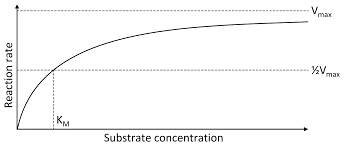
\includegraphics{img/lactate_discussion_1.png}
    \caption{Michaelis-Menten Kinetic plot of enzyme substrate reactions. }
    \label{fig:lactate_discussion}
\end{figure}
Michaelis Menten equations for reaction velocity \cite{johnson2011original}:
\begin{equation}
    E + S \xrightleftharpoons[k_{\text{off}}]{k_{\text{on}}} ES \xrightarrow{k_{cat}} E+P \quad \quad v = \frac{V_{max}[S]}{K_{M}+[S]}
\end{equation}
Enzyme kinetics can be defined partially by their Michaelis constant, Km, which describes the lactate concentration at which the current is half of that of the detection limit as seen in \autoref{fig:lactate_discussion}. In the Michaelis- Menten model, $v$ represents reaction velocity. We can take current to be proportional to $k_{cat}$, and, hence, proportional to the velocity of the H\textsubscript{2}O\textsubscript{2} production. From the Michaelis-Menten equation, as $V_{max}$ and Km are constants, the plot is hyperbolic and at higher concentrations, we can expect a decreased climb in velocity; Our calibration plot is in accordance to this. Since Michaelis-Menten kinetic models requires that immobilisation of the LOX in the matrix have no effect on its affinity for lactate, we instead approximate a value for $K_{m}$ by calculating an apparent constant $K_{m[app]}$. We can approximate $v_{max}$ $4.04\times10^{-6}$ A based on our calibration curve. This then gives a $K_{m[app]}$ proportional to the concentration where a current of $2.02\times 10\textsuperscript{-6}$A would be observed at approximately 1.0mM.\\\\
We can conclude that the Nafion membrane modified sensor is therefore useful at detecting concentrations in the range experimented. Although readings plateau in the upper range of lactate concentrations, since a patient is septic anywhere in this range- the same measures (i.e administration of antibiotics) would be taken whether the patient exhibits levels in the 3.5-4.5mM range as would be taken if levels are beyond 4.5mM.  
\subsection{Aptamer Modelling}
In this study, we have developed a novel numerical inverse laplace algorithm capable of decomposing multi-exponential chronoamperometric current signals. We show this algorithm is able to resolve rate constants up to a resolution of $k_{A} = 200s^{-1}$ and $k_{AT} = 400s^{-1}$, on simulated signals with realistic noise levels. Accurate estimates were also obtained for the coefficients, showing the accuracy of the algorithm in obtaining target concentration, [T]. These values of rate constants are closer compared to the $k_{A} = 125s^{-1}$ and $k_{AT} = 500s^{-1}$ quoted in Plaxco's study \cite{arroyo2018subsecond}.\\\\
In parallel, we develop a coarse-grained model of aptamers by assuming it as a freely-jointed chain to gain insight into the physical effects of target binding. We generate length probability distributions, and assess how the probability of a collision event $P(L<1.5nm)$ varies with Aptamer length. These estimates correlate with aptamer modelling studies in the literature \cite{uzawa2010mechanistic,uzawa2009length}.\\\\

\newpage
\section{Conclusion}





\subsection{Summary and Future Work}
\subsubsection{Future of the Microneedle Device}
Our MN biosensor has two main application purposes: (1) accessing the ISF by penetrating the skin barrier and (2) act as a platform for the recognition element.  Hence, more holistic theoretical research has been performed on skin structure and MN design considerations for translation to in-vivo testing in Appendix Part A and B.
\subsubsection{Nitrite}
 Nitrite experimentation has been shown to be repeatable in solution and can accurately determine nitrite concentration. Next steps involve using the calibration curve obtained from these experiments in serum and fresh blood samples from patients with sepsis and determine the accuracy of the detection method.\\\\
 The biosensor would then be used in large-scale trials to determine the sensitivity, specificity and positive predictive ratio of the nitrite biosensor. Improvements to the disposable electrode construction include improving on electrode stability, reducing the need for replacement over time.
\subsubsection{Hydrogen Peroxide}
Immediate future steps for hydrogen peroxide involves testing the electrochemical properties of hydrogen peroxide on disposable electrodes and/or rotating disc electrodes and implementing the electrochemical detection onto the microneedle platform. Meanwhile, an evaluation matrix should be established using calibration result obtained thus far in order for results from real-time monitoring to be well-interpreted, thus, facilitating diagnosis, evolution monitoring and prognosis prediction of sepsis.\\\\
In our study, a calibration curve with gold electrodes was produced over a range of concentrations through chronoamperometry. We have also performed coulometry to validate the theoretical concentrations for each calibration curve. Under extremely low and high hydrogen peroxide concentrations, the percentage difference between the experimental and theoretical concentrations are found to be high. Thus, a discreet consideration is required for future experimental design.
\subsubsection{Lactate}
The sensor is effective at detecting concentrations in the experimented ranges of concentration. Although the values of current plateau in the upper range of lactate concentrations ($>$4.5mM), septic patients normally exhibits levels in the 3.5-4.5mM/L range.\\\\
A Levich study of these lactate sensors would allow us to define parameters regarding mass transport and kinetics around the RDE, including the diffusion coefficient $D$ and standard rate constant $k^{\circ}$, allowing us to compare kinetics of different enzymes. This experiment would involve changing the rotational speed of the RDE and conducting voltammograms \cite{treimer2002consideration}. See \autoref{app:Lactate_future}.
\subsubsection{Aptamer Modelling}
Future work involves testing the numerical inverse laplace model on experimental chronoamperometric data to assess and study the distribution and resolution of rate constants for the aptamers tested in the lab. The model can be used as a tool to perform parameter sensitivity analysis, where we can test the effect of specific variables such as spacer length on the rate constant values. Accurate extraction of the rate constants can allow us to make more realistic chemical and physical models of the aptamers. We have currently ignored the effects of chemical forces (e.g. base to base hydrogen bonding), as well as thermodynamic considerations of the aptamer molecule. More realistic modelling can help us understand the aptamer-target interactions, which will help scientists in this field to better assess the performance of specific aptamers in molecular sensing.
\newpage



\thispagestyle{empty}
% use one column style 
\onecolumn 
\begin{appendices}
\section{Background of Skin and it's Interstitial Fluid}
\label{Appendix_A}
\subsection{Background of Skin}
As the MN device needs to penetrate the skin barrier, knowledge of it is vital. Skin is the largest organ of the human body with an average surface area of two square metres in adults \cite{brown2021histology}. Skin thickness varies depending on the body part from 0.5mm thick on the eyelids (thinnest skin) to 4.0mm thick on the heels of the feet (thickest skin) \cite{brown2021histology}. Functions of the skin include protection (against UV light, mechanical, thermal and chemical stresses, dehydration and biological threats), sensation (contains receptors that sense touch, pressure, pain and temperature), thermoregulation (contains sweat glands, hair, and adipose tissue) and metabolic functions (subcutaneous adipose tissue is involved in the production of vitamin D, and triglycerides) \cite{brown2021histology}. We focus on the basic skin structure that affects the mechanical design of MN biosensors for successful penetration. Skin is composed of three layers \cite{brown2021histology,GARCIAGUZMAN2021116148}:
\begin{enumerate}
    \item The epidermis (thin outer layer): A keratinised stratified squamous epithelial layer of the skin that is important for the protective function of the skin. Its thickness varies between 50 - 150 um \cite{GARCIAGUZMAN2021116148}. It is divided into five sublayers \cite{brown2021histology} among which are the stratum corneum (SC) which is lipophilic and the stratum basale (SB) which is hydrophilic \cite{GARCIAGUZMAN2021116148}. The SC is the outer layer of the epidermis which serves as the primary barrier between the body and the environment \cite{brown2021histology}. Sc thickness is about 10um \cite{GARCIAGUZMAN2021116148}. The SB also known as stratum germinativum, is the deepest layer of the epidermis, separated from the dermis by the basement membrane (basal lamina) and attached to the basement membrane by hemidesmosomes \cite{brown2021histology}.
    \item The dermis (thicker middle layer): The connective tissue layer of skin containing collagen and elastic fibres that is important for sensation, protection and thermoregulation. The thickness of the dermis varies between approximately 500 and 2000 um \cite{GARCIAGUZMAN2021116148}. The pressure needed to penetrate this layer is about 1-5MPa \cite{smalls2006effect}. It contains nerves, blood vessels, fibroblasts, sweat glands, hair follicles (in some areas) and derma lymph nodes \cite{GARCIAGUZMAN2021116148,brown2021histology}. 
    \item The hypodermis (inner layer): The thickest of all the three layers. It contains adipose tissue, sweat glands, nerves and blood vessels. 
\end{enumerate}
\subsection{Using ISF as the source for sepsis biomarker detection}
Most of the required mechanical properties of MN biosensors (length, shape, rigidness, and thickness among others) depend on the biofluid source. Blood is considered the primary biofluid source for analysing and acquiring biochemical information. Blood composition constantly changes as the patient’s health condition changes. The dermal and hypodermal layers of the skin contain blood vessels, thus, enabling MN biosensors the ability to perform blood analysis. However, several challenges arise from performing blood analysis: 
\begin{enumerate}
    \item There are high concentrations of interfering species present in the blood resulting in severe fouling issues for the biosensors.
    \item MN biosensors are intended for continuous monitoring, hence, the device needs to provide the most painless user experience; More painless than traditional finger pricks.
\end{enumerate}
Skin ISF has similar profiles of proteins, small molecules, and RNA to blood and contains specific biomarkers that are exclusive or sufficient compared to blood as it comes into contact with tissues, cells, and blood capillaries \cite{liu2020microneedles}. It contains the biologically relevant biomarkers required for diagnosing sepsis. Furthermore, using skin ISF as the source for sepsis biomarkers could potentially address the issues of direct blood analysis. ISF is found in the subcutaneous tissue and, hence, MNs with shorter lengths can be used to access ISF translating to painless skin insertion of the MN device. This allows the possibility for minimally invasive, continuous biomarker monitoring over a period of hours to days, or even longer and provides on-body portability and wearability. In addition, it allows compatibility with the diagnosis of infants. Skin ISF as a biofluid source will dramatically reduce the problems of surface fouling due to having lower concentrations of proteins and other large molecules \cite{heikenfeld2018lab}; This facilitates long-term electrochemical readout. In conclusion, skin ISF was determined to be the ideal choice for the source of sepsis biomarkers for our MN biosensors to enable real-time continuous monitoring of sepsis biomarkers in a minimally invasive manner. 
\section{Microneedle Design}
\subsection{Microneedle Analytical performance}
The procedures and materials used for the fabrication design of the MN sensors strongly influence the final analytical performance and in vivo suitability of the MN device. Usually, solid MNs that are externally modified are used for developing MN biosensors as it facilitates good interaction with the target biomarker \cite{calio2016polymeric,bollella2019minimally}. However, upon skin penetration, the recognition element is susceptible to friction with the skin layers and exposed to undesired molecules present in the skin which could damage or change the recognition element. Potential solutions to mitigate this include: 
\begin{enumerate}
    \item Using an external water-soluble polymeric layer that protects the recognition element from mechanical alteration during skin penetration. Once it has penetrated the skin barrier, the layer dissolves in the ISF allowing for direct exposure to the target biomarker \cite{jin2019reduced}.
    \item Internal modification of hollow MNs to provide physical protection of the recognition element during insertion and reduces unwanted contact with tissues, hence, reducing the fouling effect \cite{zhao2020silk,miller2012multiplexed}.
\end{enumerate}
Regardless of the method of incorporating the recognition element into the MN, resistance to skin insertion must be evaluated before any in vivo application to ensure the analytical performance of the MN sensor is not affected by skin insertion or once inside the skin. 
Therefore, there is a need to confirm that external calibrations performed in in-vitro experiments can be used for calibrating biomarker concentrations in skin ISF. To confirm this, the MN biosensor is inserted through an agarose hydrogel that is in contact with artificial ISF to mimic the skin system in the human body \cite{bollella2019minimally}. Then, we measure and record the signals obtained from the MN device through the agarose hydrogel at increasing biomarker concentrations in artificial ISF and compare the calibration graph before and after insertion of the MN in the gel. To better mimic the skin system in the human body, we can use animal skin fixed onto a physical support which allows contact with artificial ISF where biomarker concentrations can be manually changed instead of gel. 
% ====================================================================
\subsection{Cytotoxicity Testing}
As the MN penetrates the skin barrier and comes into contact with skin ISF, it is vital to ensure that there is no toxicity effect caused by direct contact, leaching, or detachment of the recognition element \cite{GARCIAGUZMAN2021116148}. Cytotoxicity assays can be used to assess cell viability after exposure to the recognition element and/or its different components which is compared to a control group for certain lengths of time (e.g. after 24-72 hours). The effects of direct contact between the recognition element and the cells and effects of leaching/detachment of singular components to the cells can also be examined by other experimental procedures such as cell proliferation experiments. We should also study skin inflammation and immune response after MN biosensor insertion with the latter being related to the biocompatibility of the device \cite{kim2019continuous}.
\subsection{Microneedle Shape}
The 3 essential factors to consider while developing MN biosensors are: resistance
to skin penetration, the pain inflicted on the end-user, and the location of the target biofluid \cite{GARCIAGUZMAN2021116148}. When considering resistance to skin penetration, parameters such as MN length, type of material, shape, tip angle, and insertion force are studied for developing a robust device capable of reaching the SC or deeper with minimal penetration force and, therefore, provide a more painless user-expereimence. The skin epidermis and dermis at the body region of MN application must be independently evaluated to design the MN biosensor; The different mechanical properties, depths and skin viscoelasticities have to be taken into consideration for the MN design. \\\\
An ideal MN biosensor is said to have: (1) an elegant tip shape (conical) \cite{chang2020optimal} and minimised tip radius (5-80um) to minimise the insertion force required, (2) adequate MN thickness (5-60um), base diameter (100-200um) and Young's Modulus to prevent fracture and (3) adequate MN length to reach the biofluid source (below 600 um for ISF) \cite{GARCIAGUZMAN2021116148}. The length of the MN has to be long enough to reach the target biofluid by penetrating the appropriate skin layers but not be too long to cause axial fracture, thus, a compromise has to be made. Several studies have attempted to quantify the pain experienced by volunteers as a result of MNs and MN arrays. The effect of MN length, base diameter, thickness, number of MNs per array, and tip angle, have been studied \cite{li2013optimized, gill2008effect, lee2018three}; A direct correlation between the patient's pain and MN length (up to 1450 um) and the number of MNs placed (up to 50) was observed. MN arrays with varying thickness or tip angle, up to values of 100 um and 90 degrees, respectively, no change in discomfort levels were observed. Finally, every patient indicated that the discomfort caused by MNs was always less than that caused by regular hypodermic needle insertion (outer diameter of 460 um and insertion depth of 5 mm). 
\subsection{Forces experienced by Microneedles}
MN robustness, insertion force and tip fracture force were assessed in various studies \cite{davis_landis_adams_allen_prausnitz_2004, jung-hwan, römgens_bader_bouwstra_baaijens_oomens_2014} for a range of MN tip radii, lengths, geometries and wall thickness and  wall angles. Different imaging technologies can be used to precisely assess the state of the MN tips. This includes the USB camera attached microscope. To visualise the MNs tips with a higher magnification, scanning electron microscopy (Hitachi 3500, Pleasanton, CA) was used \cite{davis_landis_adams_allen_prausnitz_2004}. Different base radii are usually not tested due to the consideration that the stress maximizes on the microneedle tip \cite{formulas_stress}. Various authors have reported a linear dependence of the tip insertion force with the interfacial area of the needle tip. An increase in wall thickness, wall angle and tip radius was found to increase the force required to fracture the microneedles; This was supported by finite element simulations and a thin shell analytical model. Most studies used the change in electrical resistance of the outermost layer of the skin to determine the penetration point of the needle due to the high chance of inaccuracy of the visual assessment. Studies on the insertion force of the microneedle through the skin were reported to be in the range of 0.08 to 3.04 N,  for tip radii of 30 to 80 mm and wall thickness of 5mm \cite{davis_landis_adams_allen_prausnitz_2004}. It has also been shown that the average insertion force for hollow microneedles did not differ much from that of solid MNs; This leads to the conclusion that a full cross-sectional area is a better representation of an inserted microneedle in the skin, rather than the annular surface area. The fracture force was determined by pressing the microneedles against a test block until fracture occurred. Fracture force measurements were taken for wall thickness ranging from 5µm-15µm, tip radii of 40-58µm and wall angles of 60-70 degrees giving fracture forces values of 0.5N-6N, , 1.5N-6N and 1.2N - 3N respectively. Decreased tip radius drastically decreased insertion force and moderately decreased fracture force while increased wall thickness and wall angle drastically increased fracture force but had no effect on the insertion force over the range of MN shape considered. Thus, fracture force depend mostly on wall thickness and only slightly on tip radius and wall angle. This is supported by theoretical considerations where an increase in wall thickness, increases the area over which the force is applied and, thus, decreases the stress on the needle. In addition, as the microneedle wall angle gets more vertical and the shape of the microneedle approaches cylindrical, a higher fraction of the stress would get oriented along the plane of the wall rather than normal to the wall, thus, increasing the fracture force. Fracture forces were shown to always be greater than the insertion forces. Therefore, using MNs of small tip radius and large wall thickness could potentially result in a 5-fold margin of safety, which  is the ratio between the insertion and fracture forces. 

\subsection{Chemical Stability of Aptamers}
Microneedle Electrochemical Aptamer based biosensors introduced into the human body will unavoidably interact with human serum. Aptamers, being single stranded oligonucleotides, are susceptible to nuclease degradation in serum, thereby affecting it's function in vivo \cite{kratschmer2017effect}. RNA has a half life on the order of seconds, prolonged to minutes/hours for DNA molecules \cite{morrissey2005activity,kurreck2002design}. Chemical Modifications to the sugars such as 2’-fluoro (2’F) or 2’-amino
(2’NH2) ribose groups on the pyrimidine residues have shown to improve serum half-life \cite{barciszewski2009locked}. Stabilizing backbone modifications can
also be incorporated into aptamers by substituting backbone phosphate linkages (PO) with sulfur-containing phosphorothioate
linkages (PS) \cite{green1995nuclease} and phosphorodiothioate linkages \cite{yang2004progress}. In addition to sugar and phosphate modifications, the 3’ end of the molecules are usually capped with an inverted
dT residue, which provides resistance to serum exonucleases \cite{dass2002cellular}.\\\\
 Serum stability is a critical feature for assessing the viability of this sensing platform for preclinical in vivo studies, however there have been a lack of comprehensive and systematic studies of the effect of composition
 on aptamer serum stability.

\newpage
\section{Nitrite Sensor Protocol} \label{app:nitrite_protocol}
\textbf{Adopted from} Electrochemical Biosensors, Raphaël Trouillon (2011), Imperial College London\\ \textbf{Prepared by} Peter Xie, James Tang, Safiyya Musa \quad  \textbf{Reviewed by} James Mcleod, Shulin Zhang
\subsection{Electrochemical Detection of Nitrite Investigations} 
\textit{Aim: To Establish baseline ability of electrode to sense nitrite in ideal conditions, between concentrations of 4-20$\mu$M (Nitrite in PBS). Serum nitrite concentrations in healthy individuals is around 1.7 $\mu$M, whereas patients infected with sepsis have higher concentrations.} \\\\
Nitrite Investigation Summary:
Differential Pulse Voltammetry (DPV) on nitrite solutions performed using the apparatus setup in Figure 1 with a 2 mm gold electrode (CHI101) as the working electrode (WE), platinum wire (CHI115) as the counter electrode (CE) and Ag/AgCl electrode (CHI111) as the reference electrode (RE). The blank electrolyte was pH 7.4 phosphate – buffered saline (PBS). The WE were polished with alumina slurry. WE is then washed with deionised water and sonicated in ethanol. DPV was performed using the PalmSens Emstat3 potentiostat with default parameters adjusted experimentally for performance.
\subsection{Reusable Gold Electrode Cleaning (Essential between Experiments)}
\begin{enumerate}
    \item Place three MicroCloth polishing pads (Buehler) into three Petri dishes
    \item Use spatula to place 1.0 $\mu$m, 0.3 $\mu$m and 0.05 $\mu$m dry alumina (Buehler) into the three plates, respectively
    \item Add distilled water to form alumina slurries
    \item Starting with the 1.0 $\mu$m plate and decreasing in size, move the 2 mm gold working electrode (CHI101) through the slurry in a figure-eight pattern, with the electrode perpendicular to the surface of the plate, and wash the electrode with deionised water after every polishing
    \item Place electrode into a bottle with 5\% ethanol and deionised water
    \item Insert bottle into VWR ultrasonic cleaning bath for 5 minutes
\end{enumerate}

\subsection{Production of Phosphate buffered solution (PBS)}
\begin{table}[H]
    \centering
    \begin{tabular}{|c|c|}
    \hline
    \textbf{Reagent} & \textbf{Mass(g)}  \\ 
    \hline
    NaCl & 8.0 \\
    KCl & 0.2 \\
    Na\textsubscript{2}HPO\textsubscript{4} & 1.44 \\
    KH\textsubscript{2}HPO\textsubscript{4} & 0.24 \\
    \hline
    \end{tabular}
 
    \label{tab:my_label}
\end{table}

To 800ml deionised water add reagents listed above. 
Confirm with pH probe that solution is pH 7.4. Adjust with HCl if necessary.
\\
Top up with deionised water to 1L.

\subsection{Preparation of Electrochemical cell}
\begin{enumerate}
    \item Circuit Wiring and Connection: • Red – working electrode • Blue – reference electrode • Black – counter electrode • Green – ground
    \item Insert 15 mL of PBS into electrochemical cell
    \item Connect nitrogen canister to bottle of 1 M KCl solution and connect bottle to cell in order to degas the PBS
    \item Rinse Ag/AgCl reference electrode (CHI111) and platinum wire counter\\ electrode (CHI115) in deionised water 
    \item Place all three electrodes into cell as shown above
    \item Connect the Palmsens potentiostat to the electrodes via crocodile clips
    \item Perform Differential pulse voltammetry
\end{enumerate}

\begin{figure}[H]
\centering
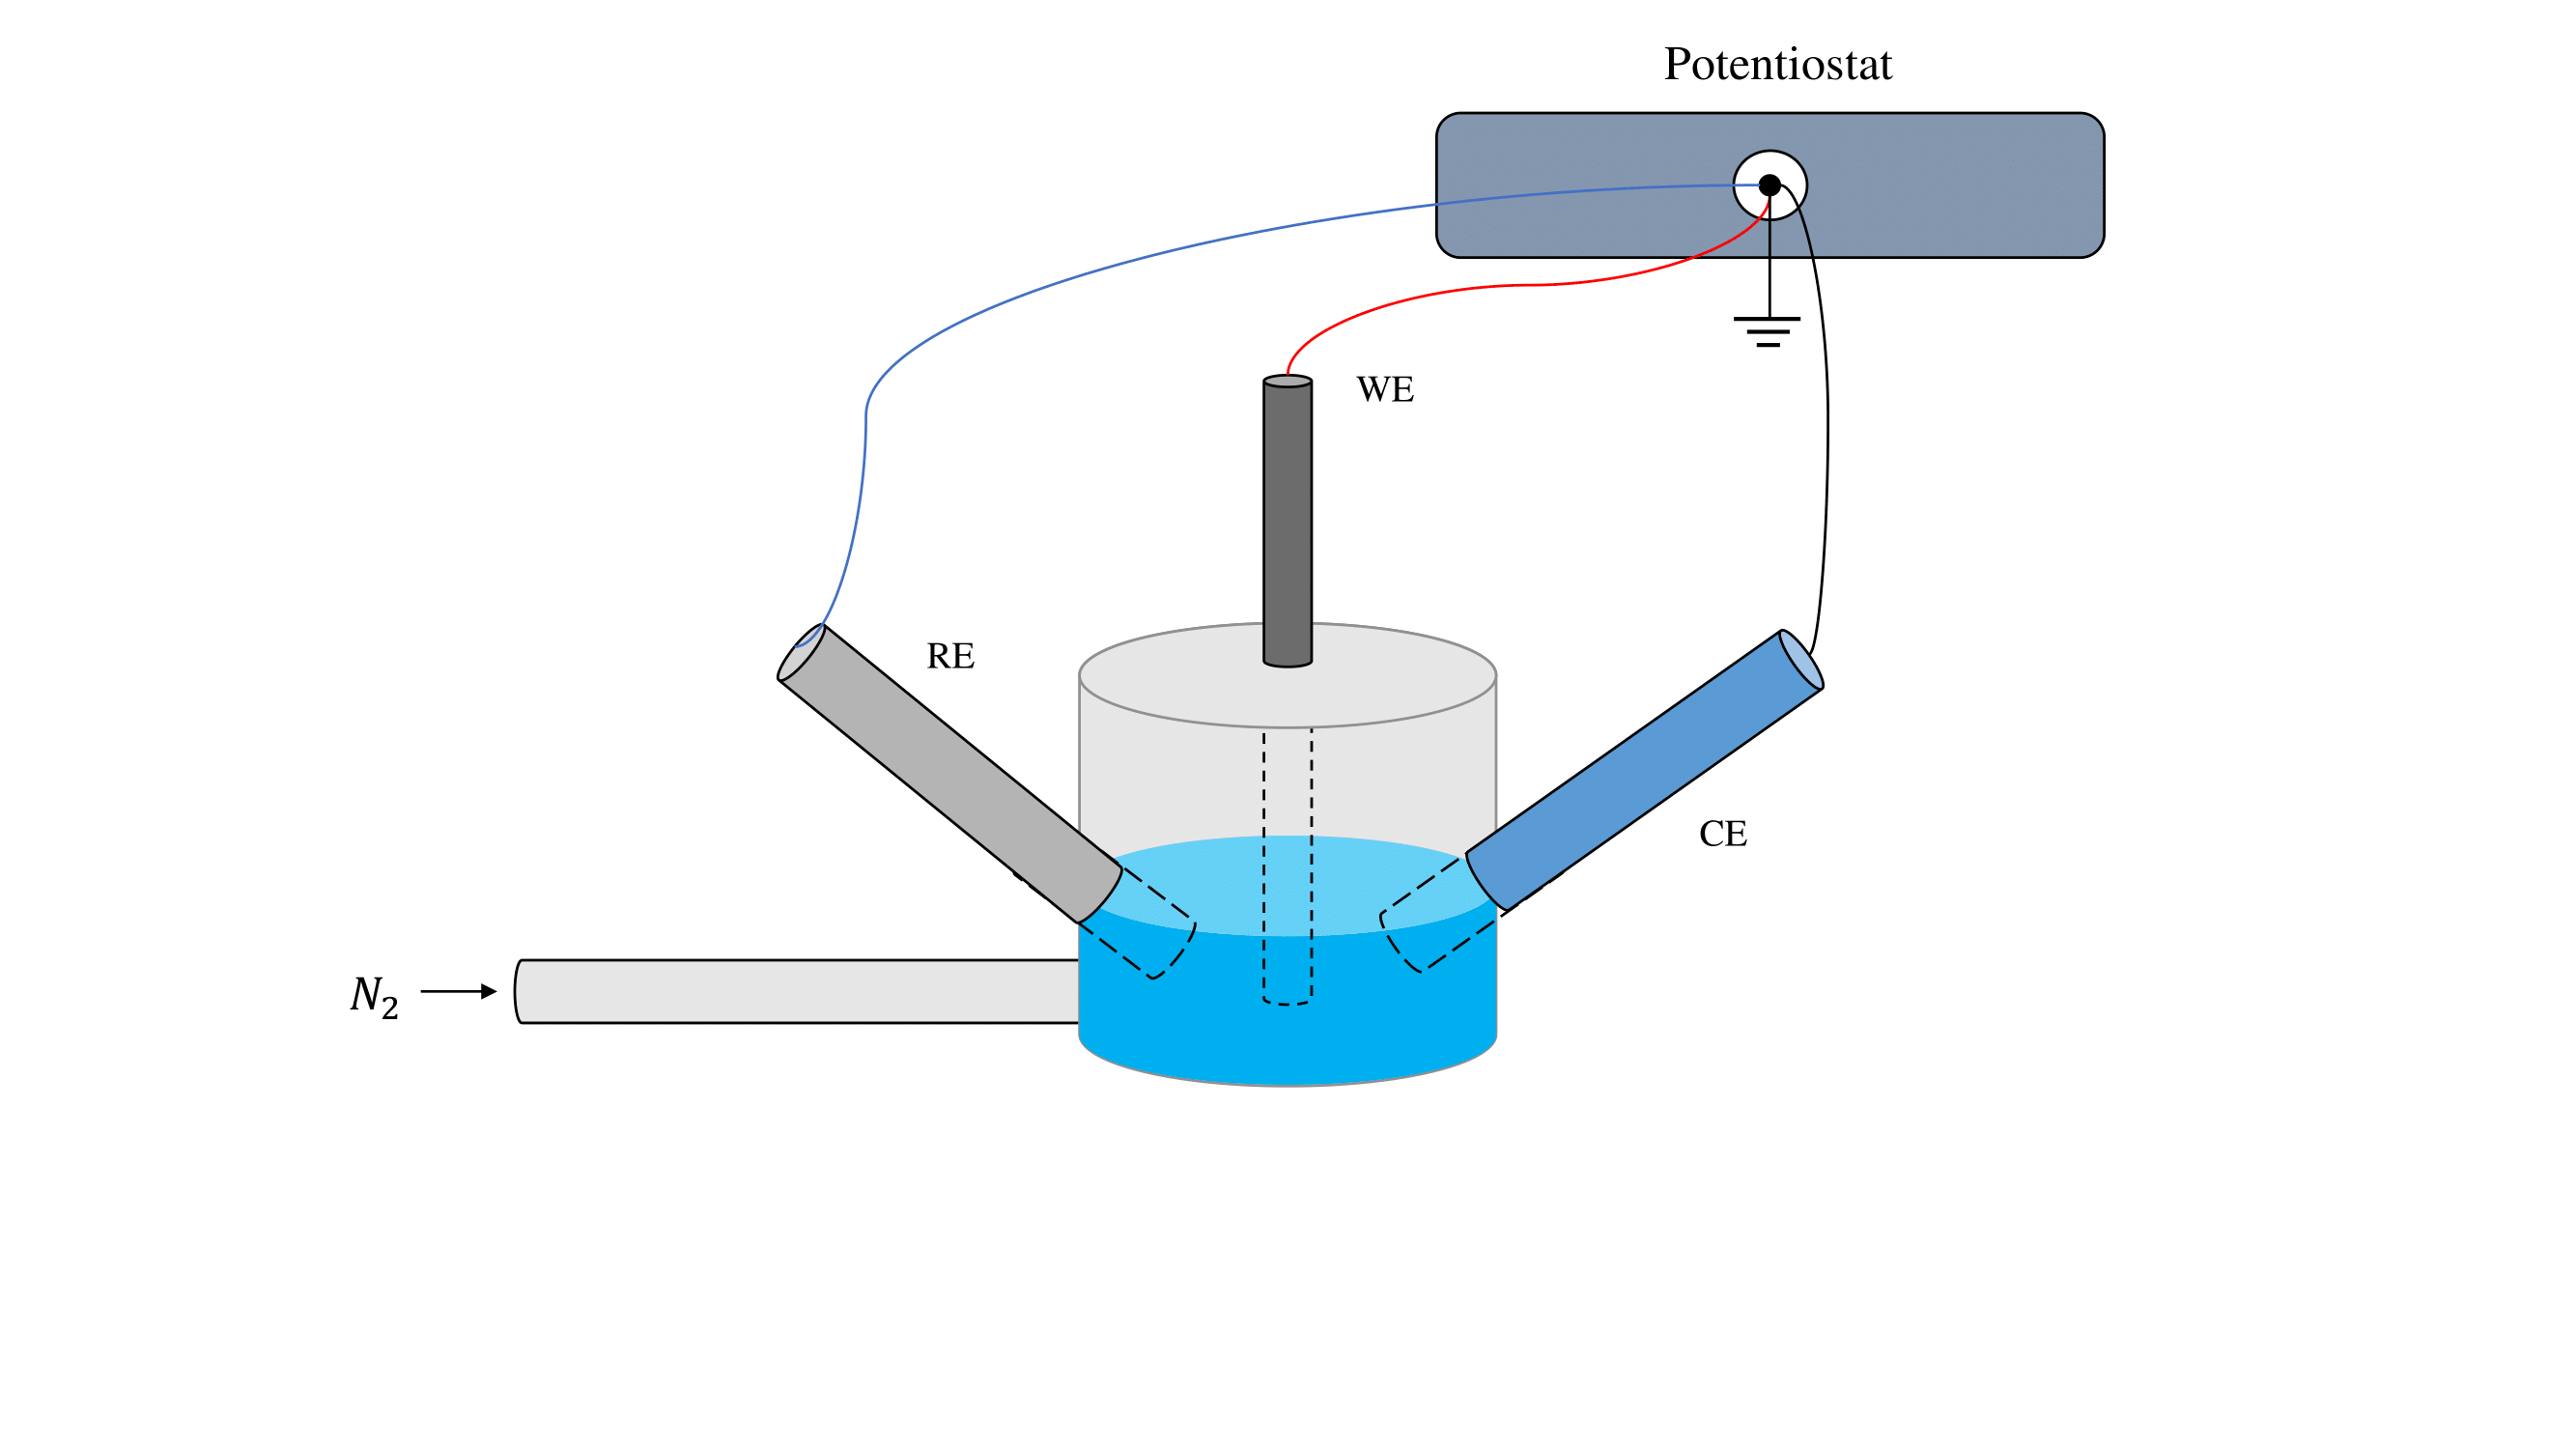
\includegraphics[height=6cm]{img/james1.png}
 \end{figure}
\textbf{Parameters for Palmsens Emstat\textsubscript{3} DPV}

\begin{table}[H]
    \centering
    \begin{tabular}{|c|c|}
    \hline
    \textbf{Parameter} & \textbf{Value}  \\ 
    \hline
    T equilibrium (s) & 10.0 \\
    Initial E (V) & 0.00 \\
    Final E (V)& 1.00 \\
    E step (V) & 0.001 \\
    E pulse/Amplitude (V) & 0.01 \\
    T pulse (V) & 0.2 \\
    Scan rate (V/s) & 0.0025 \\
    \hline
    \end{tabular}
 
    \label{tab:my_label}
\end{table}

\subsection{Production of calibration curve}

\begin{enumerate}
    \item Dissolve 17.25mg of sodium nitrite into 50 mL of PBS to produce a 10 mM sodium nitrite solution: 
    \item Run a blank DPV (run DPV without placing any of the sodium nitrite solution). 
    \item Repeat assembly of electrochemical cell a further five times pipetting 12 $\mu L$ volumes of the above sodium nitrite solution into the cell each time to give nitrite concentrations of 4 $\mu$M, 8 $\mu$M, 12 $\mu$M, 16 $\mu$M, 20 $\mu$M, 24 $\mu$M, 28 $\mu$M, 48 $\mu$M, 96$\mu$M 
    \item Perform Differential pulse voltammetry
    \item Add Sulfamic Acid, twice the number of moles as there is nitrite in the final solution, to add in excess (sulfamic acid reacts with nitrite in a 1:1 reaction).  
    \item Measure the pH of the electrochemical cell solution, and add NaOH until the pH reequilibrates to 7.4 
    \item Repeat the DPV with the original settings and investigate any changes in peak height 
    \item Construct a calibration curve by plotting peak current vs concentration of nitrite 
    
\end{enumerate}

\subsection{Albumin interference investigation}

\begin{enumerate}
    \item  Place 5.2 g of Bovine serum albumin (BSA) into a graduated bottle and add PBS until the volume inside the bottle reaches 100 mL to give a Bovine serum albumin (BSA) concentration of 52mg/ml. 
    \item Repeat Step 2 of the protocol described in Nitrite calibration curve 
    \item Construct a standard addition curve and calculate the SD and limits of detection 
    
\end{enumerate}
\subsection{Disposable gold electrode investigation}
\begin{enumerate}
    \item Wash disposable gold electrode in 75\% ethanol
    \item Produce a 15\% pHEMA solution by dissolving 250mg pHEMA in 5ml of methanol
    
    \item Add 1 drop of PDADMAC to Reference electrode and bake in oven for 1 hour at 70\textdegree{C}
    \item Add 5$\mu$L of pHEMA to Reference electrode and bake in oven for 1 hour at 70\textdegree{C}
    \item Perform Differential pulse voltammetry using the method described in nitrite investigations using the same parameters and custom testing device. Pipette solution in smaller volumes so that all electrodes are covered by the solution. Replace electrode after each DPV experiment
\end{enumerate}

%=====================================================================================
\newpage
\section{Nitrite Processing Code} \label{app:nitrite_code}
\lstinputlisting{Code/PlottingCyclicVoltammograms.m}
\lstinputlisting{Code/Plot_Calibrations_together.m}
\lstinputlisting{Code/GeneralLinearFit.m}

%=====================================================================================
\newpage
\section{Hydrogen Peroxide Electrochemical Detection Protocol} \label{app:h2o2_protocol}
\textbf{Adopted from} \href{https://pubs.rsc.org/en/content/articlelanding/2020/an/c9an02438g}{\textit{Chen and O'Hare (2020)}} \quad \textbf{Prepared by} Binghuan Li, Safiyya Musa \quad  \textbf{Reviewed by} Shulin Zhang
\subsection{PEDOT:PSS-PB Synthesis}
\textit{Aim: prepare PEDOT:PSS-PB-EG-DVS complex. Coat the working electrode with the  PEDOT:PSS-PB-EG-DVS complex.}
\begin{enumerate}
    \item Dissolve 0.03487 g ferric chloride solution in 2ml of de-ionised water (DW).
    \item 	Add PEDOT:PSS (5 ml, 0.8 wt\% PSS 43 mM PSS (monomer)) dropwise into the ferric chloride solution.
    \item Stir the solution for 2 hours, centrifuge and wash in DW twice at 8000 rpm for 10 mins.
    \item Add 20 ml (0.1 M) aqueous potassium ferrocyanide solution to the PEDOT:PSS solution.
    \item Stir the solutions for 15 minutes, centrifuge and wash in DW for three times at 8000 rpm for 10 minutes.
    \item Add 30 ml DW to disperse PEDOT:PSS.
    \item Add 20\% v/v Ethylene glycol (EG) and 10\% v/v divinyl sulfone (DVS) to the PEDOT:PSS-PB mixture to increase the mechanical stability.
    \item Apply 1.6 ul PEDOT:PSS-PB-EG-DVS on a gold working electrode (diameter 2mm). Cure in an oven at 110\textsuperscript{$\circ$}C for 1 hour.
\end{enumerate}
\subsection{Hydrogen Peroxide Solution Preparation}
\textit{Aim: set the hydrogen peroxide concentration range from 50 uM to 300 uM.}
\begin{enumerate}
    \item Dilute 9.79 M hydrogen peroxide 
    solution to 0.1 M.
    \[M_{1}V_{1} = M_{2}V_{2}\]
    \begin{itemize}
        \item $M_1$: 9.79 M, the concentration of hydrogen peroxide solution before dilution.
        \item $V_1$: 10.2 ul, the volume of the hydrogen peroxide solution before dilution.
        \item $M_2$: 0.1 M, the concentration of the hydrogen peroxide solution after dilution.
        \item $V_2$: 1 ml, the volume of the hydrogen peroxide solution after dilution.
    \end{itemize}
    
    \item Dilute 0.1 M hydrogen peroxide solution to the desired concentration.
    \begin{table}[H]
        \centering
        \begin{tabular}{|c|c|c|c|} \hline
            $M_{1}$ / uM & $V_{1}$ / ml & $M_{2}$ / M & $V_{2}$ / ul \\ \hline
            50  & 20 & 0.1 & 10 \\ \hline
            100 & 20 & 0.1 & 20 \\ \hline
            150 & 20 & 0.1 & 30 \\ \hline
            200 & 20 & 0.1 & 40 \\ \hline
            250 & 20 & 0.1 & 50 \\ \hline
            300 & 20 & 0.1 & 60 \\ \hline
        \end{tabular}
        \caption{Hydrogen peroxide concentration calculation}
        \label{tab:my_label}
    \end{table}
\end{enumerate}

\subsection{Experimental Setup}
\begin{figure}[H]
    \centering
    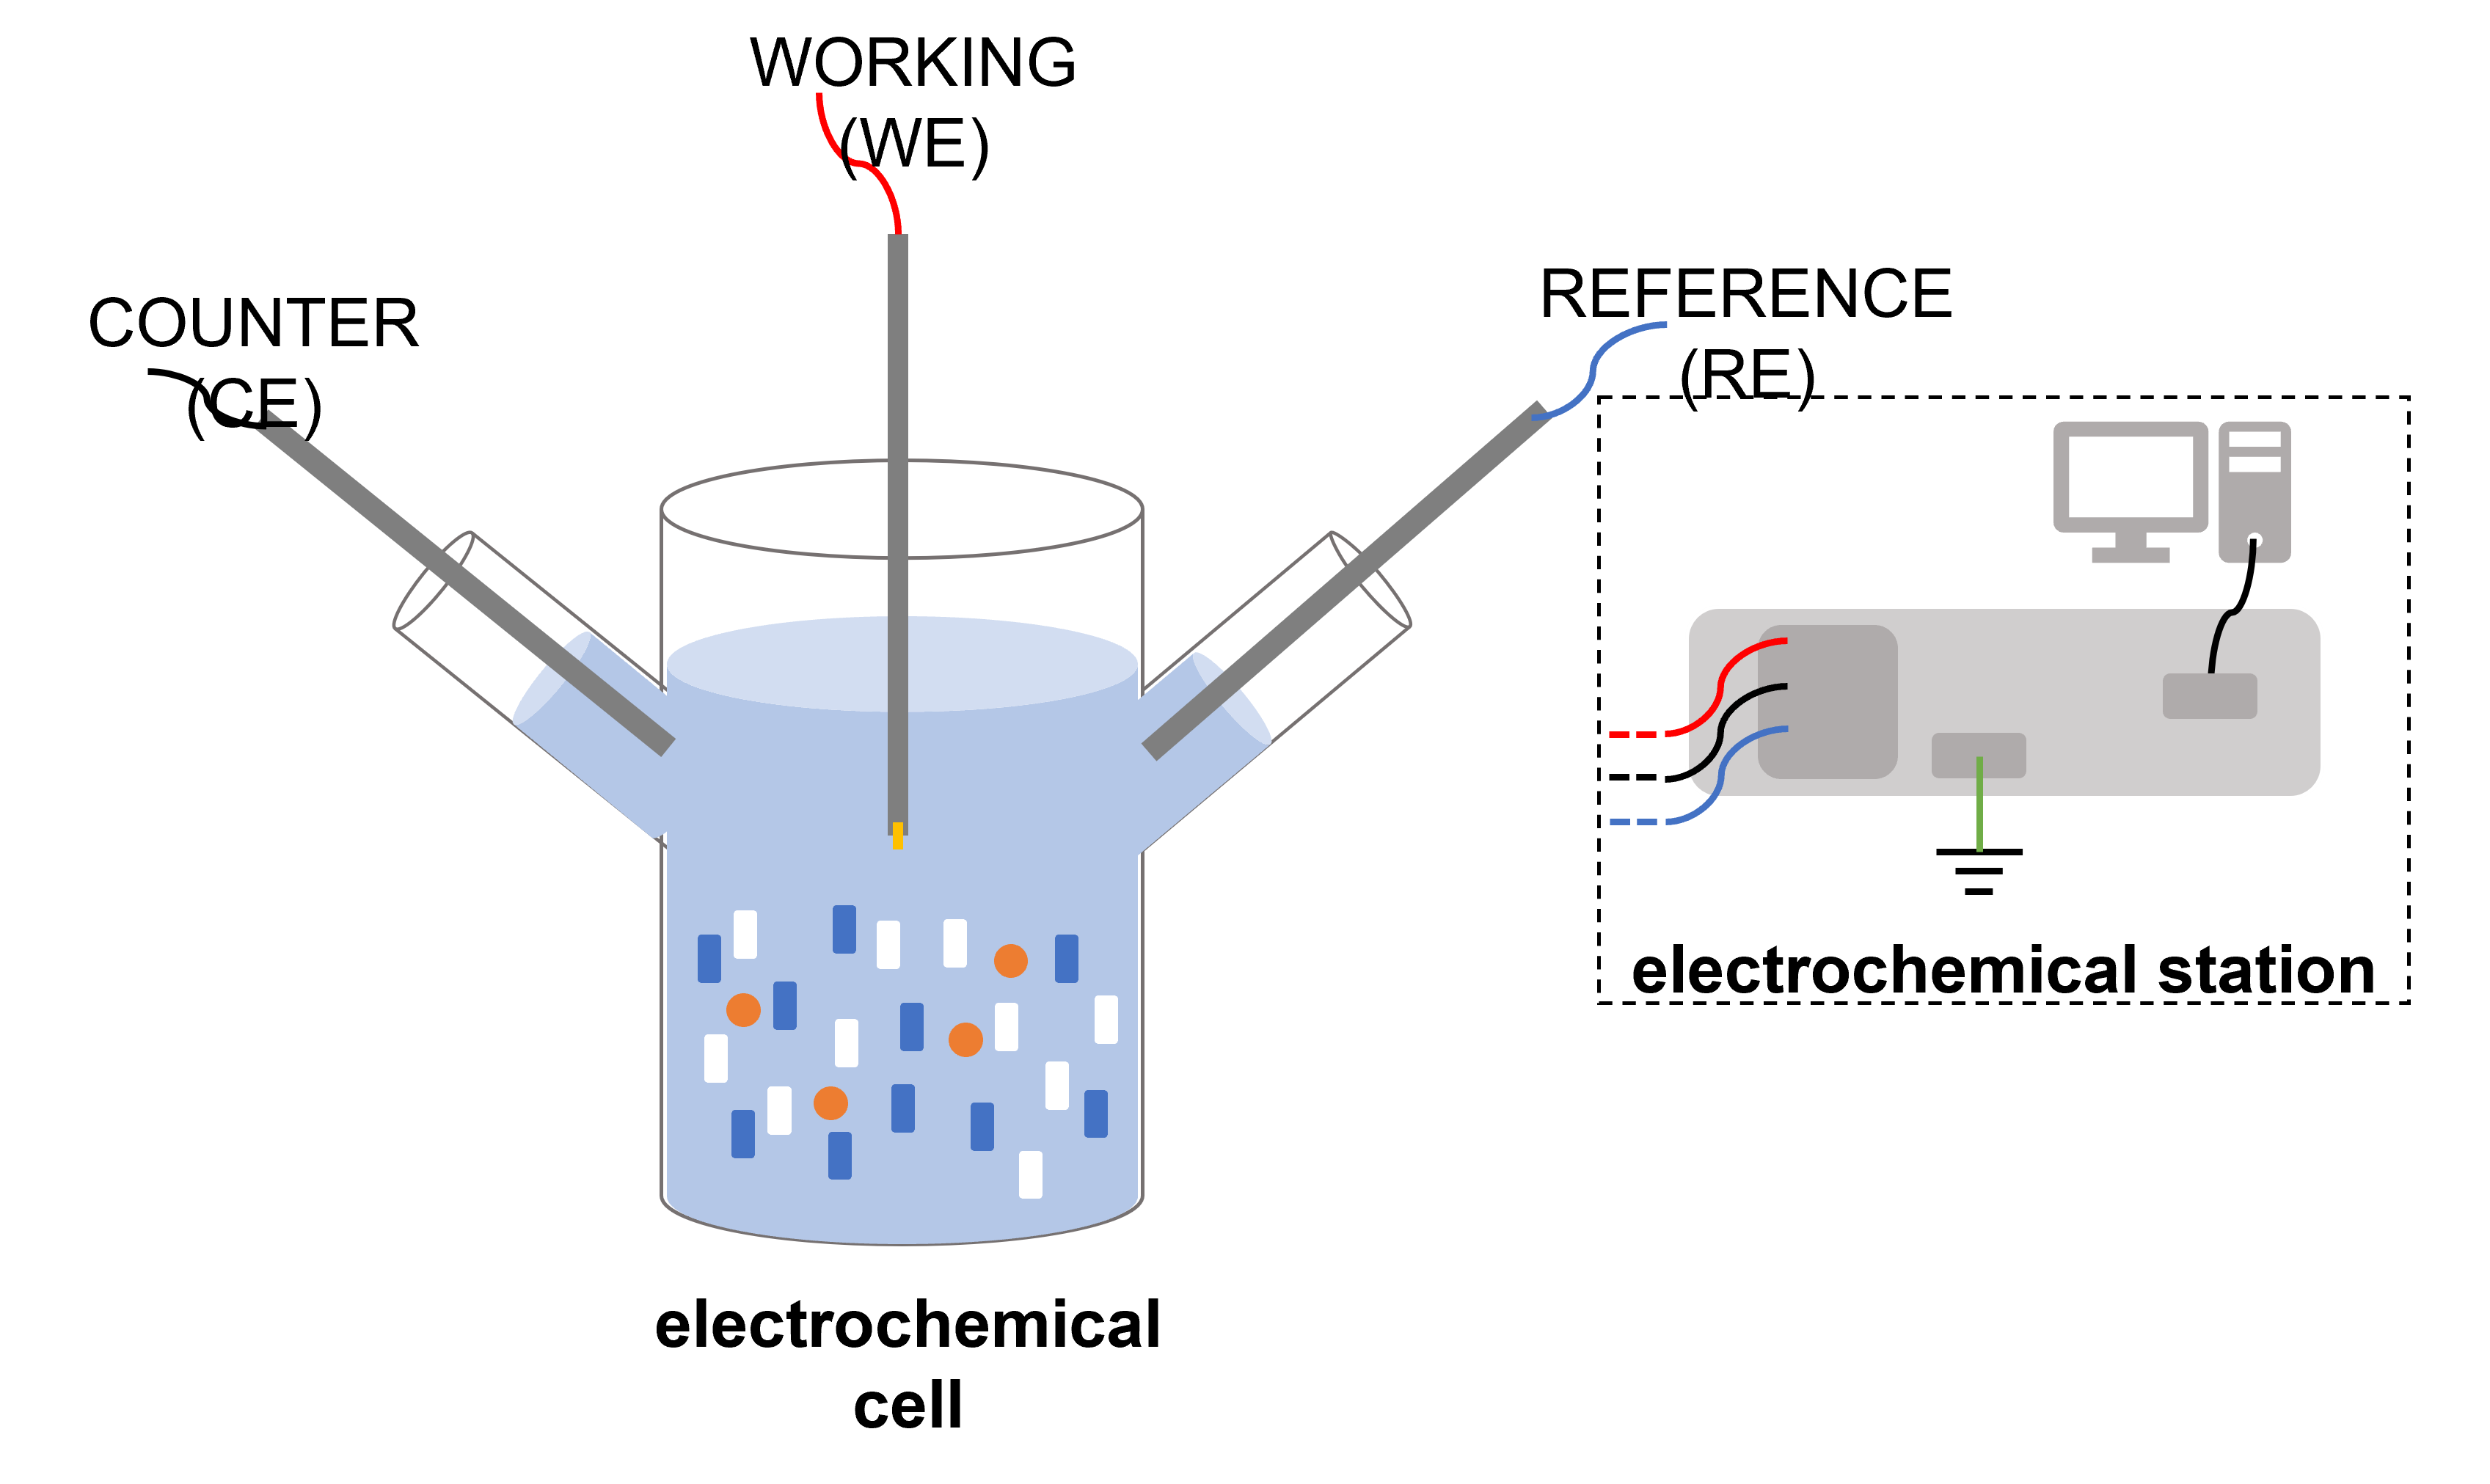
\includegraphics[width=.6\textwidth]{img/h2o2_setup.png}
\end{figure}

\subsection{Cyclic Voltammetry}
In IviumSoft\textsuperscript{\copyright}, run cyclic voltammetry  scanning in a blank buffer for 4 cycles. A starting voltage at 0.5V and an ending voltage at -0.5V  with a step increment at 1mV is applied to all scans. Scan rate is set to 100 mV/s. A stable reading is taken from the third / fourth scan. 

\subsection{Chrono Amperometry}
In IviumSoft\textsuperscript{\copyright}, run chrono amperometry scanning under each hydrogen peroxide concentration. Interval time is set to 0.03s and current range is set to 100 uA. The voltage applied to the reaction environment is set to 0.05V.

\begin{enumerate}
    \item Start the chrono amperometry scanning with the blank buffer, Waiting the data reach a stable state, pause the scanning process. 
    \item Add 10ul hydrogen peroxide solution to the buffer. Use a plastic dropper to well mix the solution.
    \item Restart the scanning. Waiting the data to be stable, pause the sampling process. 
    \item Repeat step (2) and (3) for each concentration until the concentration reaches 300 uM.
\end{enumerate} 
\subsection{Electrode Cleaning}
\begin{enumerate}
    \item Use alumina to polish the electrode (1mm, 0.3mm, 0.05mm) for 100 cycles, until no scratch can be observed on the electrode sensor surface.
    \item Rinse the electrode in de-ionised water (DIW) and clean with ultrasonic machine for 5 minutes. 
    \item No need to store in fridge.
\end{enumerate}

%=====================================================================================
\newpage
\section{Hydrogen Peroxide Coulometry} \label{app:h2o2_coulometry}
\noindent Coulometry serves as a powerful tool to amplify the signal as well as reduce the noise through integrating the amperometry current data with respect to time. By Anson equation \cite{Anson1966}, the charge can be expressed as an integral of current, as shown in \autoref{eqn:anson}. 
\begin{equation}\label{eqn:anson}
    Q(t) = \int_{t_{1}}^{t_{2}}i(t) \mathrm{d}t = \frac{nFA\sqrt{D}\sqrt{t}}{\sqrt{r}}C_{\infty}
\end{equation}
where $n$ is the number of charge transferred in the reaction, $D$ is the diffusion coefficient, $r$ is the radius of the working electrode and $A$ is the area of the working electrode.\\\\
Based on Anson equation, an improved Anson equation was proposed by Flanagan \textit{et al} \cite{Flanagan1973} by considering the edge-effect in the experiment, shown in \autoref{eqn:improved_anson}.
\begin{equation}\label{eqn:improved_anson}
    Q(t) = \frac{nFA\sqrt{D}}{\sqrt{\pi}}C_{A}\bigg( \sqrt{t}+\frac{1.92\sqrt{D}}{r}t\bigg)
\end{equation}
\noindent The realisation of coulometry is shown in the listing below.
\lstinputlisting{Code/coulometry.m}

%=====================================================================================
\newpage
\section{Lactate Sensor Protocol}
\label{app:lactate_protocol}
\textbf{Prepared by} Saylee Jangne, Safiyya Musa

\subsection{Fabrication of lactate electrode}	
\begin{enumerate}
    \item Deposit platinum black on gold electrode
        \begin{enumerate}
            \item Produce a solution of 3$\%$ w/v chloroplatinic acid and 0.005$\%$ w/v lead acetate in deionised water
            \item Apply constant current of -15 mA/cm2 for 60 s under constant stirring (vs Ag|AgCl RE and large surface area CE)
            \item Rinse thoroughly and keep wet at all times
            \item Stabilise nanoparticles by cycling in 0.5 M sulphuric acid:
                \begin{itemize}
                    \item 90 cycles -0.2 – 1.3 V at 0.1 V/s
                    \item 10 cycles -0.25 – 1.3 V at 0.05 V/s
                \end{itemize}
        \end{enumerate}
        
    \item Electropolymerisation of m-phenylenediamine (interference exclusion layer)
        \begin{enumerate}
            \item Produce a solution of 100 mM mPD in 10 mM PBS 
            \item Apply 0 V for 20 s, 0.7 V for 20 min and 0 V for 5 min (vs Ag|AgCl RE)
            \item Rinse with deionised water
        \end{enumerate}
        
    \item Coat with enzyme hydrogel
        \begin{enumerate}
            \item In 10mM of pH 7.4 PBS solution add 
                \begin{itemize}
                    \item 60 mg/ml lactate oxidase
                    \item 30 mg/ml bovine serum albumin
                    \item 2$\%$ glycerol
                    \item 60 mg/ml polyethylene glycol diglycidyl ether
                \end{itemize}
            \item Drop 4ul solution onto the electrode and after 3 mins remove 2ul
            \item Dry the sensors facing upwpards to achieve a thin film
            \item Bake in oven at 55\textsuperscript{$\circ$}C for 2 hours
        \end{enumerate}
        
    \item Coat with nafion to extend dynamic range
        \begin{enumerate}
            \item Coat electrodes with 5$\%$ solution Nafion
            \item Dry in air
        \end{enumerate}
\end{enumerate}

\subsection{Lactate Calibration Protocol}

\begin{enumerate}
    \item Electrochemical cell setup
        \begin{enumerate}
            \item Take the lactate sensor out of the freezer and hydrate by pipetting a drop of PBS on to the surface of the exposed electrode.
            \item Set up the electrochemical cell as per the diagram, ensuring the platinum and silver electrodes are in place.
            \item Add 20ml of pH 7.4 PBS to the cell 
            \item Screw the lactate sensor in to the RDE machine and suspend in solution.
            \item Connect wires to CHI potentiostat and turn the program on 0.7V for a 3 hour cycle.
            \item Turn the RDE machine on to rotate the electrode at 400rpm
            \item Allow an hour for the sensor readings to stabilise
        \end{enumerate}
        
    \item Production of lactate stock solution
        \begin{enumerate}
            \item To produce a 100mM/L solution of sodium lactate in PBS, measure 224.12mg of the sodium lactate with a weighing scale
            \item Add the lactate to 20ml of pH 7.4 PBS solution and stir gently
        \end{enumerate}
    
    \item Calibration
        \begin{enumerate}
            \item One the readings have stabilised, pipette 20uL of the lactate stock solution into the cell and record the time added- the step corresponds to the addition of 0.2mM/L lactate.
            \item Once the reading after the step has stabilised, add another 20uL
            \item Repeat the process until a concentration of 3mM/L has been reached
            \item Thereafter, pipette 100uL to achieve a concentration of 3.5mM/L
            \item Repeat the process once the reading has stabilised for 2 more additions of 100uL until 4.5mM/L has been achieved and end program
        \end{enumerate}
\end{enumerate}

%=====================================================================================
\newpage
\section{Lactate Code}
\lstinputlisting{Code/lactate.m}
%=====================================================================================
\newpage
\section{Lactate Future Considerations}
\label{app:Lactate_future}
\subsection{Enzyme selection}
Various enzymes with different kinetics can be used for electrochemical sensing of lactate. In this experiment lactate oxidase was used due to its high wealth of literature and ease of accessibility\cite{romero2010amperometric}. Alternatively Lactate Dehydrogenase (LDH) can be used which reduces lactate in the presence of NAD\textsuperscript{+}, producing NADH which can be detected by the electrode \cite{narayanan2020lactic}.
\begin{align}
    Lactate + NAD^{+} \xrightarrow{} Pyruvate + NADH + H^{+}
\end{align}
\begin{align}
    NADH \xrightarrow{} NAD + H^{+} + 2e^{-}
\end{align}
In previous experiments, LDH has shown to have a high sensitivity and limit of detection and so it would be sensible as a next step to explore the use of LDH in sensor fabrication. \\\\
A Levich study of these lactate sensors would allow us to define the parameters regarding mass transport and kinetics around the RDE, including the diffusion coefficient $D$ and standard rate constant $k^{\circ}$, allowing us to compare the kinetics of the enzymes. This experiment would involve changing the rotational speed of the RDE and conducting voltammograms \cite{treimer2002consideration}.  The Levich equation follows
\begin{equation}
    j_{L} \mathrm{(Am^{-2})} = 0.62nFD^{0.67}\mathrm{(m^{2}s^{-1})} v^{-0.166}\mathrm{(m^{2}s^{-1})}c\mathrm{(mol\ m^{-3})}\omega\mathrm{(rad \ s^{-1})}
\end{equation}
where $n$ is number of electrodes involved in reaction, $F$ is Faraday’s constant (=96,500C/mol), $D$ is diffusion constant, $v$ is kinematic velocity, $C$ is concentration of electroactive species in solution, $\omega$ is rotational speed.\\\\
From this equation we can deduce that $j_{L}$ is proportional to c (when $v$ and $\omega$ are held constant). Furthermore, for the case of mass transport to be true $j_{L}$ vs $\omega^{0.5}$ should display a linear relationship passing through the origin.
Graphically, a Levich plot yields a sigmoidal function of j against the potential for different rotational speeds. \\\\
We can then use the Levich study to apply a Koutecy exploitation whereby the inverse of the current is plotted against the rotational speed, sampled at different potentials (where there is a steep rise and plateau from the Levich plot) \cite{nikolic2000theoretical}. The linear relationship should obey the Koutecy-Levich law. 
\begin{align}
    \frac{1}{i_{L}} = \frac{1}{i_{K}}+\bigg(\frac{1}{0.620nFD^{2/3}v^{-1/6}C}\bigg)\omega^{-1/2}
\end{align}
If plotted, the rate constant can be determined by the y intercept of the graph.
For plots sampled at current on the rising portion of the Levich plot, extrapolating back to $\omega=0$ will give non-zero intercepts indicating the slow kinetics at electrode surface limits the reaction rate even at high rotational speeds (hence high mass transport). 
We can use Koutecy-Levich studies to observe the differences in enzyme kinetics for LOX and LDH sensors and make informed decisions, based on the kinetic parameters, which is a more accurate representation of live interstitial lactate levels.
%=====================================================================================
\newpage
\section{Aptamer Multiexponential Current Derivation}
\label{Aptamer_multiexp}
In this study, we assume the aptamer state as being a distribution of two states, bound and unbound. Binding-induced conformation change in the aptamer increases the electron transfer rate from $k_{A}$ to $k_{AT}$ (Fig. \ref{aptamerrate}). It is hypothesized that target binding causes an
increase of the efficiency of electron transfer (ET) between the
electrode and the redox reporter as they are moved closer together \cite{farjami2011off} (Methylene Blue \cite{arroyo2018subsecond}).\\\\
\begin{figure}[H]
    \centering
    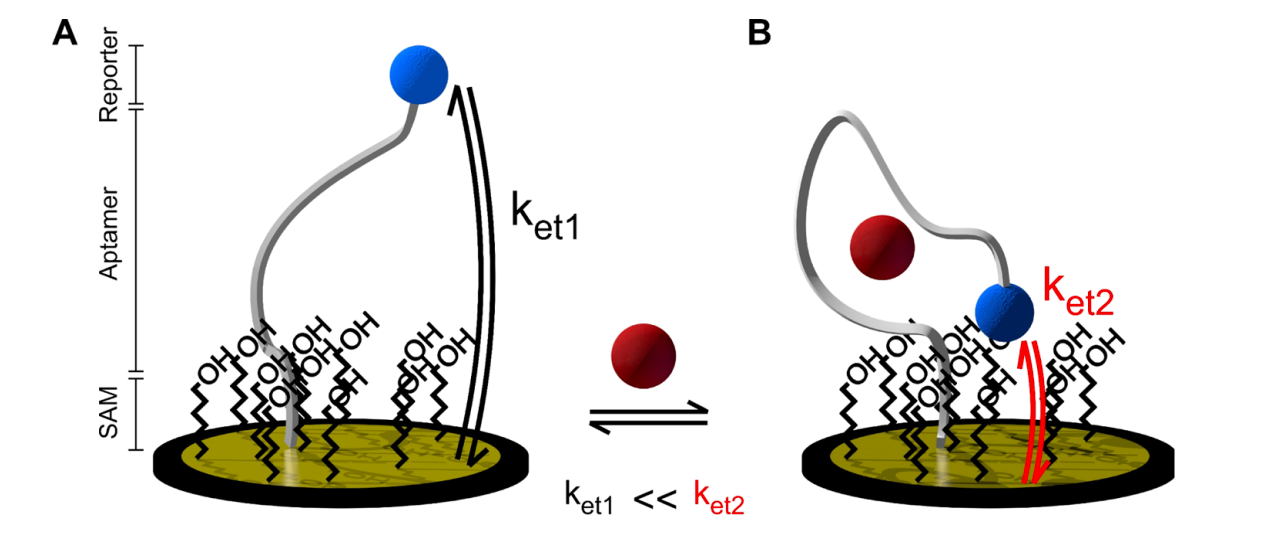
\includegraphics[width = 1.0\textwidth]{img/aptamerdiagram2.png}
    \caption{Aptamer Electron transfer rate. Increases due to Target binding to the Aptamer.\cite{arroyo2018subsecond}}
    \label{aptamerrate}
\end{figure}
Target ([T]) binding to the Aptamer ([A]), forms the aptamer-ligand complex ([AT]) as shown in the following chemical reaction:
\begin{align}
\cee{[A] + [T]  &<=> [AT]} 
\end{align}
The binding rate of the target to the aptamer is $k_{on}$ and the off-binding rate of the target to the aptamer is $k_{off}$. Assuming the system is in equilibrium, the rate of the forward reaction is equal to the rate of the backward reaction:
\begin{equation}
k_{on}[A][T] = k_{off}[AT]
\end{equation}
Using the conservation of mass for the total aptamer concentrations:
\begin{equation}
[A_{0}] = [A] + [AT]
\end{equation}
Faradaic reduction of the methylene blue reporter to leucomethylene blue occurs during chronoamperometric detection
 \cite{zhan1990mechanisms}:
\begin{align}
\cee{MB^{+} + 2e^{-} + H^{+}  &-> LMB} 
\end{align}
Electron transfer empirically follows a first order rate reaction \cite{bard1983electrochemical, forster1994electrochemistry}. Therefore the output current follows an exponential decay.
% $$ k_{ET} = -\frac{d[e^{-}]}{dt} $$
% $$ \therefore [e^{-}] = e^{-k_{ET}t} $$

\subsection{Chronoamperometric Signal}
Upon a step wave excitation in potential during chronoamperometry, the output current is a sum of exponential decay signals \cite{arroyo2018subsecond}, one due to the bound aptamer, and another due to the unbound aptamer, with the relative contributions of the exponential decays to be equal to the concentrations of the bound and unbound aptamers respectively. The two exponential decay components are likely to be a distribution, centered at the mean average value. Modelling the rate constants 'k' as a probability distribution would more physically represent the physical scenario.
$$ \frac{i}{nFA} = [AT]e^{-k_{AT}t} + [A]e^{-k_{A}t} $$
Deriving the expressions for the concentrations of the bound and unbound aptamer configurations as functions of the total aptamer concentration - we use equations (2) and (3) to derive [AT]:
$$ [AT] = \frac{k_{on}[T][A_{0}-AT]}{k_{off}} $$
$$ [AT] = \frac{k_{on}[T][A_{0}]}{k_{off}} - \frac{k_{on}[T][AT]}{k_{off}} $$
$$ [AT](1+\frac{k_{on}[T]}{k_{off}}) = \frac{k_{on}[T][A_{0}]}{k_{off}} $$
$$  [AT] = \frac{k_{on}[T]}{k_{off}+k_{on}[T]}[A_{0}] $$
Using a similar method, we can get an expression for [A], concentration of the unbound aptamer. Alternatively, we can calculate [A] using the conservation of mass formula, where [A] = [$A_{0}$]-[AT]:
$$ [A] = \frac{k_{off}}{k_{off}+k_{on}[T]}[A_{0}] $$
Final equation for the output current:\\\\
\begin{equation}
\frac{i}{nFA} = \frac{k_{on}[T]}{k_{on}[T]+k_{off}}e^{-k_{AT}t} + \frac{k_{off}}{k_{on}[T]+k_{off}}e^{-k_{A}t}
\end{equation}
\clearpage
\section{Aptamer Modelling Code} \label{app:apt_mod}
\subsection{Multiexponential Rate Extraction Code}
\lstinputlisting{Code/Rate_res_testing.m}
\newpage
\subsection{Numerical Inverse Laplace Solver}
\lstinputlisting{Code/iLaplace.m}
\newpage
\subsection{Coarse-grained Aptamer Modelling}
\lstinputlisting{Code/Chain_sim_bound_unbound_v3.m}
\newpage
\subsection{Probability from DNA length Model}
\lstinputlisting{Code/Electron_transfer_FINAL.m}
\newpage

%=====================================================================================
\section{Risk Assessment}
% \begin{table}[H]
%     \centering
    \begin{longtable}{|p{.1\textwidth}|p{.1\textwidth}|p{.1\textwidth}|p{.1\textwidth}|p{.1\textwidth}|p{.1\textwidth}|p{.08\textwidth}|p{.13\textwidth}|}\hline
        \textbf{Hazard} & \textbf{Risk} & \textbf{Likelihood} & \textbf{Severity} & \textbf{Risk rating} & \textbf{Mitigation} & \textbf{Revised risk} & \textbf{Contingency }\\ \hline
        
        Lab unavailability & Unable to test blood samples & 2 & 3 & 6 & \textit{N/A} & \textit{N/A} & Move to literature based research on how blood sampling results may differ \\ \hline
        
        Chemical shortages e.g enzyme & Cannot test new markers & 4 & 3 & 12 & \textit{N/A} & \textit{N/A} & Use pre-fabricated sensors where available or else move to literature based research \\ \hline
        
        Inadequate sensitivity (detection falls in desired detection range) & Unable to produce sufficient calibration curves & 1 & 4 & 4 & \textit{N/A} & \textit{N/A} & Produce curves until detection limit, use literature to investigate how behaviour is expected to progress beyond experimented concentrations \\ \hline
        
        Faulty equipment & Unable to conduct electrochemical tests & 3 & 5 & 15 & \textit{N/A} & \textit{N/A} & Borrow or purchase replacements\\ \hline
        
        Sodium lactate & Can cause skin and eye irritation, irritation of digestive and respiratory tract. & 2 & 3 & 6 & Wear gloves and face masks, avoid prolonged exposure. Flush eyes/skin upon contact & 1 & \textit{N/A}\\ \hline
        
        Sodium nitrite NaNO3 & Toxic if swallowed, serious eye irritation & 2 & 4 & 8 & Do not eat in lab, wear gloves and mask. Immediately seek medical attention if swallowed. & 3 & \textit{N/A}\\ \hline
        
        \pagebreak
        
        Hydrogen Peroxide solution H2O2 &  Can cause severe burn injuries on contact with skin or eyes. & 2 & 4 & 8 & Diluted samples used. Use gloves and seek medical attention in case of contact & 3 & \textit{N/A}\\ \hline
        
        
        Electrical equipment & Can overheat and malfunction. & 2 & 4 & 6 & Turn off appliances when not in use. If overheating, terminate experiments and continue after a break where possible. & 3 & \textit{N/A}\\ \hline
        
        Chemical spills & Can come in to contact with live wires causing explosions. & 2 & 4 & 8 & Keep wet experiments away from live electrical appliances, use insulated wires and small volumes of liquid. Clean any spills immediately & 3 & \textit{N/A}\\ \hline
    \end{longtable}
% \end{table}



%=====================================================================================

\end{appendices}
\newpage
\printbibliography
\end{document}